\documentclass{ctexbook}
\usepackage{amsmath,amsthm,amssymb}
\usepackage{physics}
\usepackage{esint}

\usepackage{marginnote}
\usepackage{thmtools}
\renewcommand{\listtheoremname}{定理索引}
\declaretheorem[name={推论},numberwithin=chapter]{corollary}
\declaretheorem[name={定义},numberwithin=chapter]{definition}
\declaretheorem[name={定理},numberwithin=chapter]{theorem}
\declaretheorem[name={命题},numberwithin=chapter]{proposition}

\def\diff{\textnormal{d}}
\def\e{\textnormal{e}}

\usepackage{gbt7714}
\usepackage{multicol}
\usepackage{multirow}
\usepackage{lscape}
\usepackage{pgfplots}
\pgfplotsset{compat=newest}
\usetikzlibrary{plotmarks}
\usetikzlibrary{patterns}
\usepgfplotslibrary{fillbetween}
\usepackage[colorlinks]{hyperref}

\begin{filecontents*}{ref.bib}
@Book{analysis,
    author    = {陈纪修 and 於崇华 and 金路},
    publisher = {高等教育出版社},
    title     = {数学分析},
    year      = {2019},
    address   = {北京},
    edition   = {3},
    isbn      = {978-7-04-051571-8},
}

@Book{tj,
    author    = {同济大学数学系},
    publisher = {高等教育出版社},
    title     = {高等数学},
    year      = {2014},
    address   = {北京},
    edition   = {7},
    isbn      = {978-7-04-039663-8},
}

@Book{lg,
    author    = {上海交通大学 数学系 线性代数课程组},
    publisher = {高等教育出版社},
    title     = {大学数学 线性代数},
    year      = {2012},
    address   = {北京},
    edition   = {2},
    isbn      = {978-7-04-033805-8},
}

@Book{prob,
    author    = {冯卫国 and 武爱文},
    publisher = {上海交通大学出版社},
    title     = {概率论与数理统计},
    year      = {2018},
    address   = {上海},
    edition   = {5},
    isbn      = {978-7-313-19966-9},
}

@Book{zy1000,
    author    = {张宇},
    publisher = {北京理工大学出版社},
    title     = {张宇考研数学题源探析经典1000题},
    year      = {2022},
    address   = {北京},
    isbn      = {978-7-5763-0818-1},
}

@Book{gs18,
    author    = {张宇},
    publisher = {北京理工大学出版社},
    title     = {张宇高等数学18讲},
    year      = {2022},
    address   = {北京},
    isbn      = {978-7-5673-0851-8},
}

@Book{gl2022,
    author    = {张宇},
    publisher = {北京理工大学出版社},
    title     = {张宇概率论与数理统计9讲},
    year      = {2022},
    address   = {北京},
    isbn      = {978-7-5673-0851-5},
}

@Book{xd2022,
    author    = {张宇},
    publisher = {北京理工大学出版社},
    title     = {张宇线性代数9讲},
    year      = {2022},
    address   = {北京},
    isbn      = {978-7-5673-0851-2},
}

@Misc{zx,
    author = {张旭},
    title  = {张旭微积分},
    year   = {2022},
    url    = {https://space.bilibili.com/521685904},
}
\end{filecontents*}

\begin{document}
\title{考研数学知识点}
\author{Log Creative No.0223}
\date{2022 年 10 月 9 日}
\maketitle

\begin{quotation}
    \begin{center}
        \bfseries 内\quad{}容\quad{}提\quad{}要
    \end{center}

    本书主要摘抄了 2023 年考研数学一大纲规定的定义与定理,并添加了一些注释。 
\end{quotation}

\vspace{5em}

版权所有 \copyright{} 2022,保留所有权利,请勿用于商业用途。

Copyright \copyright{} 2022, All Rights Reserved. No Commercial.

Log Creative (LC) 编号 No.0223

\tableofcontents

\part{高等数学}

\chapter{函数极限与连续}

\section{函数极限}

\begin{definition}[函数极限]
    设函数 $y=f(x)$ 在点 $x_0$ 的某个去心邻域 $O(x_0,\rho) \setminus \{x_0\}\subseteq D_f$ 中有定义,如果 $\exists A\in \mathbb{R}$,对于 $\forall \epsilon >0$,可以找到 $\delta>0$,使得当 $0<\lvert x-x_0\rvert<\delta$:
    \begin{equation}
        \lvert f(x)-A\rvert<\epsilon
    \end{equation}
    则称
    \begin{equation}
        \lim_{x\rightarrow x_0}f(x)=A
    \end{equation}
\end{definition}

\begin{definition}[单侧极限]
    设函数 $f(x)$ 在 $(x_0-\rho,x_0)$ ($\rho>0$) 上有定义,若 $\exists B\in\mathbb{R}$ 使得 $\forall \epsilon > 0$,$\exists \delta\in(0,\rho)$,$\forall x\in(x_0-\delta, x_0)$ 有
    \begin{equation}
        \lvert f(x)-B\rvert<\epsilon
    \end{equation}
    则称
    \begin{equation}
        \lim_{x\rightarrow x_0^-}f(x)=B
    \end{equation}
\end{definition}

\begin{theorem}[左右极限相等]
    函数 $f(x)$ 在 $x_0$ 点极限存在 $\Leftrightarrow$ $f(x)$ 在 $x_0$ 的左右极限存在且相等。
\end{theorem}

\begin{proposition}[函数极限性质]
    极限存在时的性质。
    \begin{description}
        \item[唯一性] 若 $A$ 和 $B$ 都是函数 $f(x)$ 在点 $x_0$ 的极限,则 $A=B$。
        \item[局部保序性] 若 $\lim_{x\rightarrow x_0}=A$,$\lim_{x\rightarrow x_0}=B$,且 $A>B$,则存在 $\delta>0$,当 $0<\lvert x-x_0\rvert<\delta$ 时,成立
        \begin{equation}
            f(x)>g(x)
        \end{equation}
        \item[局部有界性] 若 $\lim_{x\rightarrow x_0} f(x)=A$,则 $\exists\delta>0$,使得 $f(x)$ 在 $O(x_0,\delta)\setminus \{x_0\}$ 中有界。
        \item[夹逼性] 若存在 $r>0$,使得当 $0<\lvert x-x_0\rvert<r$ 时,成立
        \begin{equation}
            g(x)\leq f(x)\leq h(x)
        \end{equation}
        且 $\lim_{x\rightarrow x_0}g(x)=\lim_{x\rightarrow x_0}h(x)=A$,则 $\lim_{x\rightarrow x_0}f(x)=A$。
    \end{description}
\end{proposition}

\begin{theorem}[函数极限四则运算]
    设 $\lim_{x\rightarrow x_0}f(x)=A$,$\lim_{x\rightarrow x_0}g(x)=B$,则
    \begin{enumerate}
        \item $\lim_{x\rightarrow x_0}(\alpha f(x)+\beta g(x))=\alpha A + \beta B$,其中 $\alpha,\beta$ 是常数
        \item $\lim_{x\rightarrow x_0}(f(x)g(x))=AB$
        \item $\lim_{x\rightarrow x_0}\frac{f(x)}{g(x)}=\frac{A}{B}$ $(B\neq 0)$
    \end{enumerate}
\end{theorem}

\section{函数连续}

\begin{definition}[函数连续]
    设 $f$ 在点 $x_0$ 的某个邻域内有定义,且 $\lim_{x\rightarrow x_0}f(x)=f(x_0)$,则称 $f$ 在 $x_0$ 点连续,$x_0$ 称为 $f(x)$ 的连续点。
\end{definition}

\begin{definition}[单侧连续]
    若 $\lim_{x\rightarrow x_0^-}f(x)=f(x_0)$,则 $f$ 在 $x_0$ 处左连续。
\end{definition}

\begin{definition}[区间连续]
    若函数 $f(x)$ 在区间 $(a,b)$ 的每一点都连续,则称函数 $f(x)$ 在开区间 $(a,b)$ 上连续。

    若 $f(x)$ 在 $(a,b)$ 连续,且在左端点 $a$ 右连续,在右端点 $b$ 处左连续,则称函数 $f(x)$ 在闭区间 $[a,b]$ 上连续。
\end{definition}

\begin{definition}[不连续点]
    函数 $f(x)$ 在点 $x_0$ 连续必须满足:$f(x_0)$ 有定义且为有限值、有左极限且 $f(x_0^-)=f(x_0)$、有右极限且 $f(x_0^+)=f(x_0)$。
    \marginpar{考研中使用:第一类---跳跃间断点、可去间断点;第二类---无穷间断点、震荡间断点。}
    \begin{description}
        \item[第一类不连续点---跳跃点] 左右极限存在但不相等,$f(x_0^-)\neq f(x_0^+)$。
        \item[第二类不连续点] 左右极限至少有一个不存在。
        \item[第三类不连续点---可去间断点] $f(x_0^-)=f(x_0^+)\neq f(x_0)$ 或者 $f(x_0)$ 无定义。  
    \end{description}
\end{definition}

\begin{definition}[无穷小量]
    当 $\lim_{x\rightarrow x_0}f(x)=0$,$\lim_{x\rightarrow x_0}g(x)=0$,
    \begin{equation}
        \lim_{x\rightarrow x_0}\frac{f(x)}{g(x)}=\begin{cases}
            0, &\Rightarrow f(x)=o(g(x))\\
            c\neq 0 &\Rightarrow f(x)\sim g(x)\\
            \infty &\Rightarrow f(x)=O(g(x))
        \end{cases}
    \end{equation}
\end{definition}
\marginnote{
    $f(x)=o(1)$表示无穷小量,
    $g(x)=O(1)$表示有界量。
}

\begin{proposition}[常见等价无穷小]
    当 $x\rightarrow 0$,
    \begin{align*}
        \ln(1+x)&\sim x & e^x-1&\sim x \\
        (1+x)^a-1&\sim \alpha x & \sin x &\sim x\\
        \lim_{y\rightarrow 0}(1+y)^{\frac{1}{x}} &= \e^{\lim_{y\rightarrow 0}\frac{1}{x}\ln(1+y)}=\e^{\lim_{y\rightarrow 0}\frac{y}{x}}
    \end{align*}
\end{proposition}

\begin{proposition}[常见导数]
    \begin{align*}
        (C)^\prime &=0 &
        (x^\alpha)^\prime &=\alpha x^{\alpha - 1}\\
        (\sin x)^\prime &= \cos x &
        (\cos x)^\prime &=-\sin x\\
        (\tan x)^\prime &= \sec^2 x &
        (\cot x)^\prime &= -\csc^2 x \\
        (\sec x)^\prime &= \tan x \sec x &
        (\csc x)^\prime &= -\cot x \csc x \\
        (\arcsin x)^\prime &= \frac{1}{\sqrt[]{1-x^2}} &
        (\arccos x)^\prime &= -\frac{1}{\sqrt[]{1-x^2}} \\
        (\arctan x)^\prime &= \frac{1}{1+x^2} &
        (\textnormal{arc}\cot x)^\prime &= -\frac{1}{1+x^2} \\
        (a^x)^\prime &= a^x\ln a &
        (e^x)^\prime &= e^x \\
        (\log_a x)^\prime &= \frac{1}{x\ln a}&
        (\ln x)^\prime &=\frac{1}{x}
    \end{align*}
\end{proposition}

\begin{proposition}[双曲函数的导数*]
    \begin{align*}
        \textnormal{sh}x &= \frac{\e^x-\e^{-x}}{2} &
        \textnormal{ch}x &= \frac{\e^x+\e^{-x}}{2}\\
        \textnormal{th}x &= \frac{\e^x-\e^{-x}}{\e^x+\e^{-x}} = \frac{\textnormal{sh}x}{\textnormal{ch}x} &
        \textnormal{cth}x&= \frac{1}{\textnormal{th}x}=\frac{\textnormal{ch}x}{\textnormal{sh}x}\\
        (\textnormal{sh}x)^\prime&=\textnormal{ch}x &
        (\textnormal{ch}x)^\prime&=\textnormal{sh}x\\
        (\textnormal{th}x)^\prime&=\frac{1}{\textnormal{ch}^2x}=\textnormal{sech}^2 x &
        (\textnormal{cth}x)^\prime&=-\frac{1}{\textnormal{sh}^2x}=\textnormal{csch}^2 x\\
        (\textnormal{sh}^{-1}x)^\prime&=\frac{1}{\sqrt{1+x^2}} &
        (\textnormal{ch}^{-1}x)^\prime&=\frac{1}{\sqrt{x^2-1}}\\
        (\textnormal{th}^{-1}x)^\prime&=\frac{1}{1-x^2}
    \end{align*}

    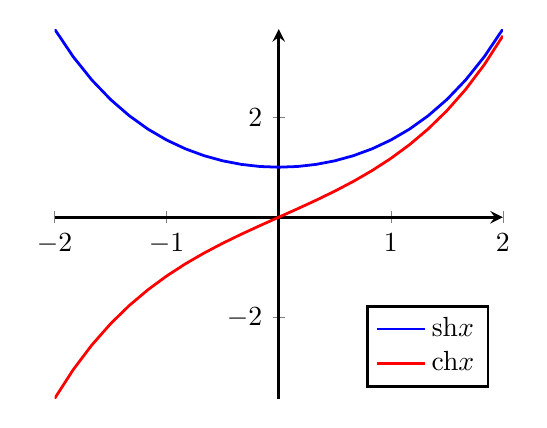
\begin{tikzpicture}
        \begin{axis}[no markers,domain=-2:2,line width=1pt,axis x line=middle,axis y line=middle,width=0.6\textwidth,legend pos={south east}]
            \addplot+ {(exp(x)+exp(-x))/2};
            \addplot+ {(exp(x)-exp(-x))/2};
            \legend{\textnormal{sh}$x$,\textnormal{ch}$x$}
        \end{axis}
    \end{tikzpicture}
    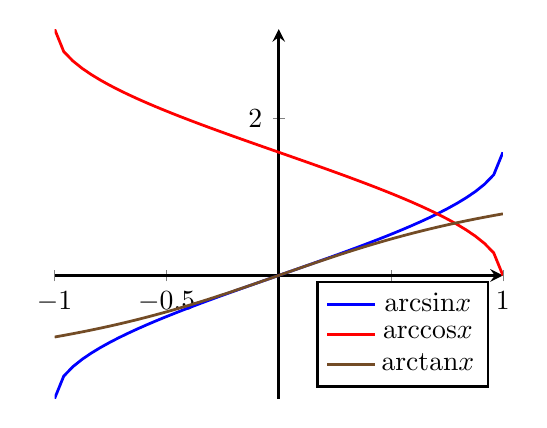
\begin{tikzpicture}
        \begin{axis}[no markers,domain=-1:1,samples=50,line width=1pt,axis x line=middle,axis y line=middle,width=0.6\textwidth,legend pos={south east}]
            \addplot+ {rad(asin(x))};
            \addplot+ {rad(acos(x))};
            \addplot+ {rad(atan(x))};
            \legend{\textnormal{arcsin}$x$,\textnormal{arccos}$x$,\textnormal{arctan}$x$}
        \end{axis}
    \end{tikzpicture}

    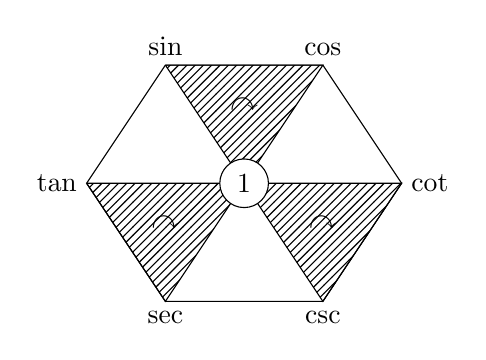
\begin{tikzpicture}[font=\normalfont]
        \path[pattern=north east lines,draw] (-1,1) -- (1,1) -- (0,-0.5) -- (-1,1);
        \path[pattern=north east lines,draw] (-2,-0.5) -- (0,-0.5) -- (-1,-2) -- (-2,-0.5);
        \path[pattern=north east lines,draw] (0,-0.5) -- (2,-0.5) -- (1,-2) -- (0,-0.5);
        \node[circle,draw,fill=white] (v2) at (0,-0.5) {1};
        \draw (-1,1) node [above] (v1) {sin} -- (1,1) node [above] (v3) {cos} -- (2,-0.5) node [right] {cot}-- (1,-2) node [below] {csc} -- (-1,-2) node [below] {sec} -- (-2,-0.5) node [left] (v4) {tan} -- cycle;
        \node at (0,0.5) { $\curvearrowright$ };
        \node at (-1,-1) { $\curvearrowright$ };
        \node at (1,-1) { $\curvearrowright$ };
    \end{tikzpicture}
    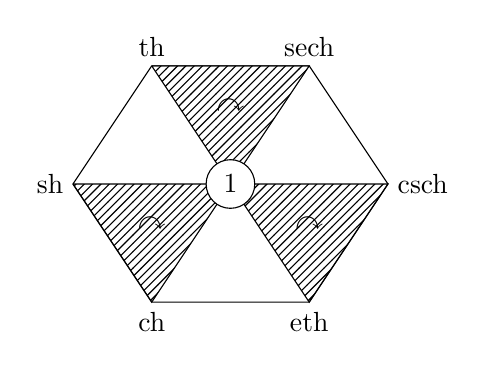
\begin{tikzpicture}[font=\normalfont]
        \path[pattern=north east lines,draw] (-1,1) -- (1,1) -- (0,-0.5) -- (-1,1);
        \path[pattern=north east lines,draw] (-2,-0.5) -- (0,-0.5) -- (-1,-2) -- (-2,-0.5);
        \path[pattern=north east lines,draw] (0,-0.5) -- (2,-0.5) -- (1,-2) -- (0,-0.5);
        \node[circle,draw,fill=white] (v2) at (0,-0.5) {1};
        \draw (-1,1) node [above] (v1) {th} -- (1,1) node [above] (v3) {sech} -- (2,-0.5) node [right] {csch}-- (1,-2) node [below] {eth} -- (-1,-2) node [below] {ch} -- (-2,-0.5) node [left] (v4) {sh} -- cycle;
        \node at (0,0.5) { $\curvearrowright$ };
        \node at (-1,-1) { $\curvearrowright$ };
        \node at (1,-1) { $\curvearrowright$ };
    \end{tikzpicture}
\end{proposition}

\section{微分中值定理及其应用}

\begin{theorem}[费马引理]
    设 $x_0$ 是 $f(x)$ 的一个极值点,且 $f(x)$ 在 $x_0$ 处导数存在,则
    \begin{equation}
        f^\prime(x_0)=0
    \end{equation}
\end{theorem}

\begin{theorem}[罗尔定理]
    \marginnote{可以用来讨论导数方程根的个数问题。}
    设函数 $f(x)$ 在闭区间 $[a,b]$ 上连续,在开区间 $(a,b)$ 上可导,且 $f(a)=f(b)$,则至少 $\exists \xi \in (a,b)$ 使得
    \begin{equation}
        f^\prime(\xi)=0
    \end{equation}
\end{theorem}

\begin{theorem}[拉格朗日中值定理]
    设函数 $f(x)$ 在闭区间 $[a,b]$ 上连续,在开区间 $(a,b)$ 上可导,则至少存在一点 $\xi\in (a,b)$ 使得
    \begin{equation}
        f^\prime(\xi)=\frac{f(b)-f(a)}{b-a}
    \end{equation}
\end{theorem}

\begin{theorem}[柯西中值定理]
    设 $f(x)$ 和 $g(x)$ 都在闭区间 $[a,b]$ 上连续,在开区间 $(a,b)$ 上可导,且对于任意 $x\in(a,b)$,$g^\prime(x)\neq 0$。则至少存在一点 $\xi\in(a,b)$,使得
    \begin{equation}
        \frac{f^\prime(\xi)}{g^\prime(\xi)}=\frac{f(b)-f(a)}{g(b)-g(a)}
    \end{equation}
\end{theorem}

\marginnote{
    证明需要用到“参数形式函数的求导公式”
    \begin{equation}
        \frac{\diff y}{\diff x}=\frac{\frac{\diff y}{\diff t}}{\frac{\diff x}{\diff t}} = \frac{f^\prime (t)}{g^\prime (t)}
    \end{equation}    
}

\begin{theorem}[洛必达法则]
    设函数 $f(x)$ 和 $g(x)$ 在 $(a,a+d]$ 上可导($d$ 是某个正常数),且 $g^\prime(x)\neq 0$。若此时有
    \begin{equation}
        \lim_{x\rightarrow a^+}f(x)=\lim_{x\rightarrow a^+}g(x)=0
    \end{equation}
    或
    \begin{equation}
        \lim_{x\rightarrow a^+}g(x)=\infty
    \end{equation}
    且 $\lim_{x\rightarrow a^+}\frac{f^\prime(x)}{g^\prime(x)}$存在(可以是有限数或$\infty$),则成立
    \begin{equation}
        \lim_{x\rightarrow a^+}\frac{f(x)}{g(x)} = \lim_{x\rightarrow a^+}\frac{f^\prime(x)}{g^\prime (x)}
    \end{equation}
\end{theorem}

\begin{theorem}[泰勒公式]
    设 $f(x)$ 在 $x_0$ 处有 $n$ 阶导数,则存在 $x_0$ 的一个邻域,对于该邻域中的任一点 $x$,成立
    \begin{equation}  
        f(x)=f(x_0)+f^\prime(x_0)(x-x_0)+\frac{f^{\prime\prime}(x_0)}{2!}(x-x_0)^2+\cdots+\frac{f^{(n)}(x_0)}{n!}(x-x_0)^n+r_n(x)
    \end{equation}
    其中皮亚诺余项 $r_n(x)=o\left((x-x_0)^n\right)$。当 $x_0=0$ 时又称为马克劳林公式。
\end{theorem}

\begin{proposition}[常见泰勒级数]
    \marginpar{展开原则:$\frac{A}{B}$ 是上下同阶原则;$A-B$ 是幂次最低原则。}
    \begin{align*}
        e^x & = 1 + x + \frac{x^2}{2!} + \frac{x^3}{3!} + \cdots + \frac{x^n}{n!} + r_n(x) \\
        \sin x &=x - \frac{x^3}{3!} + \frac{x^5}{5!} - \cdots + (-1)^n\frac{x^{2n+1}}{(2n+1)!} + r_{2n+2}(x) \\
        \cos x &=1 - \frac{x^2}{2!} + \frac{x^4}{4!} - \cdots + (-1)^n\frac{x^{2n}}{(2n)!}+r_{2n+1}(x)\\
        \tan x &= x + \frac{x^3}{3} + \cdots
    \end{align*}
    \begin{align*}
        (1+x)^\alpha &= 1 + \alpha x + \binom{\alpha}{2}x^2 + \binom{\alpha}{3}x^3 + \cdots + \binom{\alpha}{n}x^n + r_n(x)\\
        \frac{1}{1-x} &= 1 + x + x^2 + \cdots + x^n + \cdots = \sum_{n=0}^\infty x^n & \lvert x \rvert < 1 \\
        \frac{1}{1+x} &= 1 - x + x^2 - \cdots + (-1)^nx^n + \cdots = \sum_{n=0}^\infty (-1)^n x^n & \lvert x \rvert < 1 \\
        \ln(1+x) &=  x - \frac{x^2}{2} + \frac{x^3}{3} - \frac{x^4}{4} + \cdots + (-1)^{n-1}\frac{x^n}{n} + o(x^n) & -1 < x \leq 1 \marginnote{待定系数求导法} \\
        \ln(1-x) &= -x - \frac{x^2}{2} - \cdots - \frac{x^n}{n} - \cdots & -1\leq x<1\\
        \arctan x &= x - \frac{x^3}{3} + \frac{x^5}{5} - \cdots + (-1)^n\frac{x^{2n+1}}{2n+1} + o\left(x^{2n+2}\right) & x \rightarrow 0 \\
        \arcsin x &= x + \frac{x^3}{6} + \cdots
    \end{align*}
\end{proposition}

\section{微积分基本定理}

\begin{theorem}[可变上界导数]
    设 $f(x)$ 在 $[a,b]$ 上可积,作函数
    \begin{equation}
        F(x) = \int_{a}^x f(t) \diff t, \quad x\in [a,b]
    \end{equation}
    则
    \begin{enumerate}
        \item $F(x)$ 是 $[a,b]$ 上的连续函数
        \item 若 $f(x)$ 在 $[a,b]$ 上连续,则 $F(x)$ 在 $[a,b]$ 上可微,且有
        \begin{equation}
            F^\prime(x)=f(x)
        \end{equation}
        而且
        \begin{equation}
            \left(\int_a^xf(t)dt\right)^\prime=f(x)
        \end{equation}
    \end{enumerate}
\end{theorem}

\begin{theorem}[牛顿--莱布尼茨公式]
    设 $f(x)$ 在 $[a,b]$ 上连续,$F(x)$ 是 $f(x)$ 在 $[a,b]$ 上的一个原函数,则成立
    \begin{equation}
        \int_{a}^b f(x)dx=F(b)-F(a)=\left.F(x)\right|_{a}^b
    \end{equation}
\end{theorem}

\chapter{数列极限}

\begin{theorem}[数列极限]
    设 $\{x_n\}$ 是一给定数列,$a$ 是一个实常数。如果对于 $\forall\epsilon>0$,可以找到$N\in\mathbb{N}_+$,使得当 $n>N$ 时,成立
    \begin{equation}
        \lvert x_n-a\rvert<\epsilon
    \end{equation}
    则称数列 $\{x_n\}$ 收敛于 $a$(或称 $a$ 是数列 $\{x_n\}$ 的极限),记为
    \begin{equation}
        \lim_{x\rightarrow\infty}x_n=a
    \end{equation}
\end{theorem}

\begin{theorem}[收敛数列的性质]
    收敛数列的极限必惟一、必有界、保序性、夹逼性。
\end{theorem}

\begin{theorem}[数列极限的四则运算]
    设 $\lim_{n\rightarrow\infty}x_n=a$,$\lim_{n\rightarrow\infty}y_n=b$,则
    \begin{enumerate}
        \item $\lim_{n\rightarrow\infty}(\alpha x_n+\beta y_n)=\alpha a+\beta b$
        \item $\lim_{n\rightarrow\infty}(x_ny_n)=ab$
        \item $\lim_{n\rightarrow\infty}\left(\frac{x_n}{y_n}\right)=\frac{a}{b}(b\neq 0)$
    \end{enumerate}
\end{theorem}

\begin{theorem}[收敛准则]
    单调有界数列必定收敛。
\end{theorem}

\begin{proposition}[黎曼 $\zeta$ 函数]
    \begin{equation}
        a_n=\sum_{i=1}^n \frac{1}{i^p}\quad (p>0)
    \end{equation}
    当 $p>1$ 时,数列 $\{a_n\}$ 收敛;当 $0<p\leq 1$ 时,数列 $\{a_n\}$ 是正无穷大量。
    \begin{equation}
        b_n=a_n - \ln n
    \end{equation}
    则 $\{b_n\}$ 收敛。
\end{proposition}

\begin{proposition}[自然对数的数列不等式]
    \begin{equation}
        \left(1+\frac{1}{n}\right)^n<\e<\left(1+\frac{1}{n}\right)^{n+1}
    \end{equation}
    或者是
    \begin{equation}
        \frac{x}{1+x}<\ln(1+x)<x\quad (x>0)
    \end{equation}
\end{proposition}

\chapter{一元函数微分学}

\begin{definition}[微分]
    对函数 $y=f(x)$ 定义域中的一点 $x_0$,若存在一个只与 $x_0$ 有关,而与 $\Delta x$ 无关的数 $g(x_0)$,使得当 $\Delta x\rightarrow 0$ 时恒成立关系式
    \begin{equation}
        \Delta x = g(x_0)\Delta x+o(\Delta x)
    \end{equation}
    则称 $f(x)$ 在 $x_0$ 处的微分存在,或称 $f(x)$ 在 $x_0$ 处可微。若函数 $y=f(x)$ 在某一区间上的每一点都可微,则称 $f(x)$ 在该区间上可微。
\end{definition}

\begin{definition}[导数]
    若函数 $y=f(x)$ 在其定义域中的一点 $x_0$ 处极限
    \begin{equation}
        \lim_{\Delta x\rightarrow 0}\frac{\Delta y}{\Delta x}=\lim_{\Delta x\rightarrow 0}\frac{f(x_0+\Delta x)-f(x_0)}{\Delta x}
    \end{equation}
    存在,则称 $f(x)$ 在 $x_0$ 处可导,并称这个极限值为 $f(x)$ 在 $x_0$ 处的导数,记为 $f^\prime(x_0)$。若函数 $y=f(x)$ 在某一区间上的每一点都可导,则称 $f(x)$ 在该区间上可导。
\end{definition}

\begin{definition}[单侧导数]
    根据极限存在的定义,函数 $f(x)$ 在 $x_0$ 处可导的充分必要条件是相应的左极限
    \begin{equation}
        f^\prime_{-}(x_0)=\lim_{\Delta x\rightarrow 0-}\frac{f(x_0+\Delta x)-f(x_0)}{\Delta x}
    \end{equation}
    和右极限
    \begin{equation}
        f^\prime_{+}(x_0)=\lim_{\Delta x\rightarrow 0+}\frac{f(x_0+\Delta x)-f(x_0)}{\Delta x}
    \end{equation}
    存在并且相等。
\end{definition}

\begin{theorem}[反函数求导定理]
    若函数 $y=f(x)$ 在 $(a,b)$ 上连续、严格单调、可导并且 $f^\prime(x)\neq 0$,记 $\alpha =\min(f(a+),f(b-))$,$\beta=\max(f(a+),f(b-))$,则它的反函数 $x=f^{-1}(y)$ 在 $(\alpha,\beta)$ 上可导,且有
    \begin{equation}
        [f^{-1}(y)]^\prime =\frac{1}{f^\prime(x)}
    \end{equation}
\end{theorem}

\begin{definition}[高阶导数]
    设函数 $y=f(x)$ 的 $n-1$ 阶导数 $f^{(n-1)}(x)(n=2,3,\cdots)$ 仍是个可导函数,则它的导数 $[f^{(n-1)}(x)]^\prime$ 被称为 $f(x)$ 的 $n$ 阶导数,记为
    \begin{equation}
        f^{(n)}(x)
    \end{equation}
    并称 $f(x)$ 是 $n$ 阶可导函数或者 $f(x)$ 的 $n$ 阶导数存在。
\end{definition}

\begin{theorem}[线性组合函数的高阶导数]
    设 $f(x)$ 和 $g(x)$ 都是 $n$ 阶可导的,则对任意常数 $c_1$ 和 $c_2$,它们的线性组合 $c_1f(x)+c_2g(x)$ 也是 $n$ 阶可导的,且满足如下的线性运算关系
    \begin{equation}
        [c_1f(x)+c_2g(x)]^{(n)}=c_1f^{(n)}(x)+c_2g^{(n)}(x)
    \end{equation}
\end{theorem}

\begin{theorem}[Leibniz 公式]
    设 $f(x)$ 和 $g(x)$ 都满足 $n$ 阶可导函数,则它们的积函数也 $n$ 阶可导,且成立公式
    \begin{equation}
        [f(x)\cdot g(x)]^{(n)}=\sum_{k=0}^n \binom{n}{k}f^{(n-k)}(x)g^{(k)}(x)
    \end{equation}    
\end{theorem}

\begin{theorem}[一阶导数与单调性的关系]
    设函数 $f(x)$ 在区间 $I$ 上可导,则 $f(x)$ 在 $I$ 上单调增加的充分必要条件是:对任意的 $x\in I$ 有 $f^\prime(x)\geq 0$。特别地,若对于任意 $x\in I$ 有 $f^\prime(x)>0$,则 $f(x)$ 在 $I$ 上严格单调增加。
\end{theorem}

\begin{definition}[下凸函数]
    设函数 $f(x)$ 在区间 $I$ 上有定义,若对于 $I$ 中的任意两点 $x_1$ 和 $x_2$,和任意的 $\lambda\in(0,1)$,都有
    \begin{equation}
        f(\lambda x_1+(1-\lambda)x_2)\leq \lambda f(x_1)+(1-\lambda)f(x_2)
    \end{equation}
    则称 $f(x)$ 是 $I$ 上的下凸函数。
\end{definition}

\begin{theorem}[二阶导数与凸性的关系]
    设函数 $f(x)$ 在区间 $I$ 上二阶可导,则 $f(x)$ 在区间 $I$ 上是下凸函数的充分必要条件是:对于任意 $x\in I$ 有 $f^{\prime\prime}(x)\geq 0$。特别地,若对于任意 $x\in I$ 有 $f^{\prime\prime}(x)>0$,则 $f(x)$ 在 $I$ 上是严格下凸函数。
\end{theorem}

\begin{definition}[拐点]
    曲线在该点两侧的凸性相反,也就是说,它们是曲线上凸与下凸的分界点。我们称这样的点为曲线的拐点。
\end{definition}

\begin{theorem}[拐点的判定与性质]
    设 $f(x)$ 在区间 $I$ 上连续,$(x_0-\delta,x_0+\delta)\subseteq I$。
    \begin{enumerate}
        \item 设 $f(x)$ 在 $(x_0-\delta,x_0)$ 与 $(x_0,x_0+\delta)$ 上二阶可导。若 $f^{\prime\prime}(x)$ 在 $(x_0-\delta, x_0)$ 与 $(x_0,x_0+\delta)$ 上符号取反,则点 $(x_0,f(x_0))$ 是曲线 $y=f(x)$ 的拐点;否则不是拐点。
        \item 设 $f(x)$ 在 $(x_0-\delta,x_0+\delta)$ 上二阶可导,若点 $(x_0,f(x_0))$ 是曲线 $y=f(x)$ 的拐点,则 $f^{\prime\prime}(x_0)=0$。
    \end{enumerate}
\end{theorem}

\begin{definition}[驻点]
    使 $f^\prime (x)=0$ 的点称为 $f(x)$ 的驻点。
\end{definition}

\begin{definition}[渐近线]
    若曲线 $y=f(x)$ 上的点 $(x,f(x))$ 到直线 $y=ax+b$ 的距离在 $x\rightarrow +\infty$ 或 $x\rightarrow -\infty$ 时趋于零,则称直线 $y=ax+b$ 是曲线 $y=f(x)$ 的一条渐近线。当 $a=0$ 时称为水平渐进线,否则称为斜渐近线。直线 $y=ax+b$ 是曲线 $y=f(x)$ 的渐近线的充分必要条件为($x\rightarrow -\infty$ 时同理可得)
    \begin{equation}
        \lim_{x\rightarrow +\infty}[f(x)-(ax+b)]=0
    \end{equation}
    其中
    \begin{align}
        a&=\lim_{x\rightarrow +\infty}\frac{f(x)}{x}\\
        b&=\lim_{x\rightarrow +\infty}[f(x)-ax]
    \end{align}
    如果
    \begin{equation}
        \lim_{x\rightarrow a+}f(x)=\pm \infty
    \end{equation}
    或
    \begin{equation}
        \lim_{x\rightarrow a-}f(x)=\pm \infty
    \end{equation}
    则称直线 $x=a$ 是曲线 $y=f(x)$ 的一条垂直渐近线。
\end{definition}

\begin{definition}[曲率半径]
    曲率 
    \begin{equation}
        k=\frac{y^{\prime\prime}}{\left[1+(y^\prime)^2\right]^{\frac{3}{2}}}        
    \end{equation}
    曲率半径
    \begin{equation}
        R = \frac{1}{k}
    \end{equation}
\end{definition}

\chapter{一元函数积分学}

\section{不定积分}

\begin{definition}[不定积分]
    若在某个区间上,函数 $F(x)$ 和 $f(x)$ 成立关系
    \begin{equation}
        F^\prime(x)=f(x)
    \end{equation}
    或等价地,
    \begin{equation}
        \diff(F(x))=f(x)\diff x
    \end{equation}
    则称 $F(x)$ 是 $f(x)$ 在这个区间上的一个原函数。$f(x)$ 原函数的全体称为这个函数的不定积分,记作
    \begin{equation}
        \int f(x)\diff x = F(x) + C
    \end{equation}
\end{definition}

\begin{theorem}[不定积分的线性性]
    若函数 $f(x)$ 和 $g(x)$ 的原函数都存在,则对任意常数 $k_1$ 和 $k_2$,函数 $k_1f(x)+k_2f(x)$ 的原函数也存在,且有
    \begin{equation}
        \int [k_1f(x)+k_2g(x)]\diff x=k_1\int f(x)\diff x+k_2\int g(x)\diff x
    \end{equation}
    此式应当理解为等式两端所表示的函数族相同。另外,当 $k_1=k_2=0$ 时,等式右端应理解为常数 $C$。
\end{theorem}

\begin{proposition}[常用不定积分公式]
    \begin{align*}
        &\text{微分} && \text{不定积分} \\
        &\diff(\e^x)=\e^x\diff x & &\int \e^x\diff x = \e^x + C \\
        &\diff(\ln x)=\frac{\diff x}{x} & &\int \frac{\diff x}{x}\diff x=\ln\lvert x\rvert + C\\
        &\diff(x^\alpha)=\alpha x^{\alpha-1}\diff x & &\int x^\alpha \diff x=\frac{1}{\alpha+1}x^{\alpha+1}+C & (\alpha\neq 1)\\
        &\diff(\sin x)=\cos x & &\int \cos x\diff x=\sin x + C\\
        &\diff(\cos x)=-\sin x & &\int \sin x\diff x=-\cos x + C\\
        &\diff(\tan x)=\sec^2 x & &\int \sec^2 x\diff x=\tan x + C\\
        &\diff(\cot x)=-\csc^2 x & &\int \csc^2 x\diff x=-\cot x + C\\
        &\diff(\sec x)=\tan x\sec x\diff x & &\int \tan x\sec x\diff x=\sec x + C\\
        &\diff(\csc x)=-\cot x\csc x\diff x & &\int \cot x\csc x\diff x=-\csc x+C\\
        &\diff(\arcsin x)=\frac{\diff x}{\sqrt{1-x^2}}& &\int \frac{\diff x}{\sqrt[]{1-x^2}}=\arcsin x+C\\
        &\diff(\arctan x)=\frac{\diff x}{1+x^2}& &\int \frac{\diff x}{1+x^2}=\arctan x+C
    \end{align*}
\end{proposition}

\begin{proposition}[换元积分法]
    \begin{enumerate}
        \marginpar{例子(凑微元):\begin{align*}&\int\tan x\diff x\\&=\int \frac{\sin x}{\cos x}\diff x\\&=-\int\frac{\diff(\cos x)}{\cos x}\\&=-\ln\lvert\cos x\rvert+C\end{align*}}
        \item 在不定积分 $\int f(x)\diff x$ 中,若 $f(x)$ 可以通过等价变形化成 $\tilde{f}(g(x))g^\prime(x)$,而函数 $\tilde{f}(u)$ 的原函数 $\tilde{F}(u)$ 是容易求的。则
        \begin{equation}
            \begin{aligned}
                \int f(x)\diff x&=\int \tilde{f}(g(x))g^\prime(x) \diff x=\int \tilde{f}(g(x))\diff g(x)\\
                &= \int \tilde{f}(u)\diff u = \tilde{F}(u)+C = \tilde{F}(g(x)) + C
            \end{aligned}
        \end{equation}
        \marginpar{例子(凑函数):\begin{align*}&\int\sqrt[]{a^2-x^2}\diff x\\&=a^2\int\cos^2t\diff t\\&\left(x=a\sin t, -\frac{\pi}{2}\leq t\leq \frac{\pi}{2}\right)\end{align*}}
        \item 若不定积分 $\int f(x)\diff x$ 不能直接求出,但能够找到一个适当的变量代换 $x=\varphi(t)$(要求 $x=\varphi(t)$ 的反函数 $t=\varphi^{-1}(x)$ 存在),将原式化为
        \begin{equation}
            \int f(x)dx = \int f(\varphi(t)) \diff \varphi(t) = \int f(\varphi(t))\varphi^\prime(t)\diff t
        \end{equation}
        而 $f(\varphi(t))\varphi^\prime(t)$ 的原函数 $\tilde{F}(t)$ 是容易求的。
        \begin{equation}
            \int f(x)dx = \tilde{F}(t)+C = \tilde{F}(\varphi^{-1}(x))+C
        \end{equation}
    \end{enumerate}
\end{proposition}

\begin{proposition}[分部积分法]
    对任意两个可微的函数 $u(x),v(x)$ 成立关系式
    \begin{equation}
        \int u(x)\diff [v(x)]=u(x)v(x) - \int v(x)\diff[u
        (x)]
    \end{equation}
    也即
    \begin{equation}
        \int u(x)v^\prime(x)\diff x=u(x)v(x)-\int v(x)u^\prime(x)\diff x
    \end{equation}
    就是分部积分公式。

    对应的定积分形式为:设 $u(x)$ 和 $v(x)$ 在区间 $[a,b]$ 上又连续导数,则
    \begin{equation}
        \int_a^b u(x)v^\prime(x)\diff x=[u(x)v(x)]\bigg|_a^b-\int_a^b v(x)u^\prime(x)\diff x
    \end{equation}
\end{proposition}

\begin{proposition}[基本积分表]
    \begin{align*}
        &\int x^\alpha \diff x=\begin{cases}
            \frac{1}{\alpha+1}x^{\alpha+1}+C, & \alpha\neq -1,\\
            \ln\lvert x\rvert+C,&\alpha=-1
        \end{cases} & &\int \ln x\diff x=x(\ln x-1)+C\\
        &\int a^x\diff x=\frac{a^x}{\ln a}+C & &\int \e^x\diff x=\e^x+C\\
        &\int \sin x\diff x=-\cos x+C & &\int \cos x\diff x=\sin x+C\\
        &\int \tan x\diff x=-\ln\lvert\cos x\rvert+C& &\int\cot x\diff x=\ln\lvert \sin x\rvert +C\\
        &\int \sec x\diff x=\ln\lvert \sec x+\tan x\rvert+C& &\int \csc x\diff x=\ln\lvert\csc x-\cot x\rvert+C\\
        &\int \frac{\diff x}{\sqrt[]{a^2-x^2}}=\arcsin\frac{x}{a}+C& &\int \frac{\diff x}{\sqrt[]{x^2\pm a^2}}=\ln\left\vert x+\sqrt[]{x^2\pm a^2}\right\vert + C\\
        &\int \frac{\diff x}{x^2-a^2}=\frac{1}{2a}\ln\left\vert\frac{x-a}{x+a}\right\vert + C& &\int \frac{\diff x}{x^2+a^2}=\frac{1}{a}\arctan\frac{x}{a}+C\\
        &\int \sqrt[]{a^2-x^2}\diff x=\frac{1}{2}x\sqrt[]{a^2-x^2}+\frac{a^2}{2}\arcsin\frac{x}{a}+C\\
        &\int \sqrt[]{x^2\pm a^2}\diff x=\frac{1}{2}\left(x\sqrt[]{x^2+a^2}\pm a^2\ln\left\vert x+\sqrt[]{x^2\pm a^2}\right\vert\right) + C\\
        &\int_0^{2\pi}\sin^nx\diff x=\begin{cases}
            0, & n\text{为正奇数}\\
            4\cdot\frac{n-1}{n}\cdot\frac{n-3}{n-2}\cdot\cdots\cdot\frac{1}{2}\cdot\frac{\pi}{2}& n\text{为正偶数}
        \end{cases}\\
        &\int_0^{2\pi}\cos^nx\diff x=\int_0^{2\pi}\sin^nx\diff x
    \end{align*}
\end{proposition}

\begin{theorem}[代数学基本定理]
    $n$ 次实多项式 $q_n(x)$ 在复数域上恰有 $n$ 个根。设它的全部实根为 $\alpha_1,\alpha_2,\cdots,\alpha_i$,重数分别为 $m_1,m_2,\cdots,m_i$,全部复根为 $\beta_1\pm\textnormal{i}\gamma_1,\beta_2\pm\textnormal{i}\gamma_2,\cdots,\beta_j\pm\gamma_j$,其重数分别为 $n_1,n_2,\cdots,n_j$。
    \begin{equation}
        \sum_{k=1}^i m_k+2\sum_{k=1}^j n_k=n
    \end{equation}
    记 $\xi_k=-\beta_k, \eta_k^2=\beta_k^2+\gamma_k^2 (\xi_k^2<\eta_k^2)$,则在实数域上可将 $q_n(x)$ 因式分解为
    \begin{equation}
        q_n(x)=\prod_{k=1}^i(x-\alpha_k)^{m_k}\cdot\prod_{k=1}^j(x^2+2\xi_kx+\eta_k^2)^{n_k}
    \end{equation}
\end{theorem}

\begin{theorem}[有理函数真分式分解]
    设有理函数 $\frac{p(x)}{q(x)}$ 是真分式。
    \begin{enumerate}
        \item 多项式 $q(x)$ 有 $k$ 重实根 $\alpha$,即 $q(x)=(x-\alpha)^kq_1(x), q_1(\alpha)\neq 0$。则存在实数 $\lambda$ 与多项式 $p_1(x)$,$p_1(x)$ 的次数低于 $(x-\alpha)^{k-1}q_1(x)$ 的次数,成立
        \begin{equation}
            \frac{p(x)}{q(x)}=\frac{\lambda}{(x-\alpha)^k}+\frac{p_1(x)}{(x-\alpha)^{k-1}q_1(x)}
        \end{equation}
        \item 多项式 $q(x)$ 有 $l$ 重共轭复根 $\beta\pm\textnormal{i}\gamma$,即 $q(x)=(x^2+2\xi x+\eta^2)^lq^*(x)$,$q^*(\beta\pm\textnormal{i}\gamma)\neq 0$,其中 $\xi=-\beta,\eta^2=\beta^2+\gamma^2(\xi^2<\eta^2)$。则存在实数 $\mu,\nu$ 和多项式 $p^*(x)$,$p^*(x)$ 的次数低于 $(x^2+2\xi x+\eta^2)^{l-1}q^*(x)$ 的次数,成立
        \begin{equation}
            \frac{p(x)}{q(x)}=\frac{\mu x+\nu}{(x^2+2\xi x+\eta^2)^l}+\frac{p^*(x)}{(x^2+2\xi x+\eta^2)^{l-1}q^*(x)}
        \end{equation}
    \end{enumerate}
    最终,可将有理函数分解为
    \begin{equation}
        \frac{p_m(x)}{q_n(x)}=\sum_{k=1}^i\sum_{r=1}^{m_k}\frac{\lambda_{kr}}{(x-\alpha_k)^r}+\sum_{k=1}^j\sum_{r=1}^{n_k}\frac{\mu_{kr}x+\nu_{kr}}{(x^2+2\xi_kx+\eta^2_k)^r}
    \end{equation}
\end{theorem}

\begin{proposition}[有理函数不定积分]
    \begin{align}
        \int\frac{(x-\alpha)^n}{\diff x}&=\begin{cases}
            \ln|x-\alpha|+C, &n=1\\
            -\frac{1}{n-1}\cdot\frac{1}{(x-\alpha)^{n-1}}+C,&n\geq 2
        \end{cases}\\
        \int\frac{\mu x+\nu}{(x^2+2\xi x+\eta^2)^n}\diff x &=\frac{\mu}{2}\int\frac{2x+2\xi}{(x^2+2\xi x+\eta^2)^n}\diff x+(\nu-\mu\xi)\int\frac{\diff x}{(x^2+2\xi x+\eta^2)^n}
    \end{align}
\end{proposition}

\begin{proposition}[可化为有理函数不定积分]
    \begin{align}
        \int R\left(x,\sqrt[n]{\frac{\xi x+\eta}{\mu x+\nu}}\right)\diff x&\xrightarrow[x=\phi(t)=\frac{-\nu t^n+\eta}{\mu t^n-\xi}]{t=\sqrt[n]{\frac{\xi x+\eta}{\mu x+\nu}}} \int R\left(\frac{-\nu t^n+\eta}{\mu t^n-\xi},t\right)\phi^\prime (t)\diff t\\
        \int R(\sin x,\cos x)\diff x&\xrightarrow{t=\tan\frac{x}{2}}\left\{\begin{aligned}
            \sin x&=2\sin\frac{x}{2}\cos\frac{x}{2}=\frac{2t}{1+t^2}\\
            \cos x&=\cos^2\frac{x}{2}-\sin^2\frac{x}{2}=\frac{1-t^2}{1+t^2}\\
            \diff x&=2(\arctan t)=\frac{2\diff t}{1+t^2}
        \end{aligned}
        \right\}\\
        &\rightarrow \int R\left(\frac{2t}{1+t^2},\frac{1-t^2}{1+t^2}\right)\frac{2}{1+t^2}\diff t
    \end{align}
\end{proposition}

\section{定积分}

\begin{definition}[定积分]
    设 $f(x)$ 是定义于 $[a,b]$ 上的有界函数,在 $[a,b]$ 上任意取分点 $\{x_i\}_{i=0}^n$,作为一种划分
    \begin{equation}
        P:a=x_0<x_1<x_2<\cdots<x_n=b
    \end{equation}
    并任意取点 $\xi_i\in[x_{i-1},x_i]$。记小区间 $[x_{i-1},x_i]$ 的长度为 $\Delta x_i=x_i-x_{i-1}$,并令 $\lambda=\max_{1\leq i\leq n}(\Delta x_i)$,若当 $\lambda\rightarrow 0$ 时,极限
    \begin{equation}
        \lim_{\lambda\rightarrow 0}\sum_{i=1}^n f(\xi_i)\Delta x_i
    \end{equation}
    存在,且极限值既与划分 $P$ 无关,又与对 $\xi_i$ 的取法无关,则称 $f(x)$ 在 $[a,b]$ 上 Riemann 可积。极限值被称为 $f(x)$ 在区间 $[a,b]$ 上的定积分,记为
    \begin{equation}
        I=\int_a^b f(x)\diff x
    \end{equation}
\end{definition}

\begin{proposition}[定积分的性质]
    设 $f(x)$ 和 $g(x)$ 在 $[a,b]$ 上都可积。
    \begin{description}
        \item[线性性] $k_1$ 和 $k_2$ 是常数,则函数 $k_1f(x)+k_2g(x)$ 在 $[a,b]$ 上也可积
        \begin{equation}
            \int_a^b [k_1f(x)+k_2g(x)]\diff x=k_1\int_a^b f(x)\diff x+k_2\int_a^b g(x)\diff x
        \end{equation}
        
        \item[乘积可积性] $f(x)\cdot g(x)$ 在 $[a,b]$ 上也可积。
        \item[保序性] 在 $[a,b]$ 上恒有 $f(x)\geq g(x)$,则
        \begin{equation}
            \int_a^b f(x)\diff x\geq \int_a^b g(x)\diff x
        \end{equation}
        \item[绝对可积性] $|f(x)|$ 在 $[a,b]$ 上也可积,且成立
        \begin{equation}
            \left\vert\int_a^b f(x)\diff x\right\vert\leq\int_a^b\lvert f(x)\rvert\diff x
        \end{equation}
        \item[区间可加性] 对任意点 $c\in[a,b]$,
        \begin{equation}
            \int_a^b f(x)\diff x=\int_a^c f(x)\diff x+\int_c^b f(x)\diff x
        \end{equation}
    \end{description}
\end{proposition}

\begin{theorem}[积分第一中值定理]
    设 $f(x)$ 和 $g(x)$ 都在 $[a,b]$ 上可积,$g(x)$ 在 $[a,b]$ 上不变号,则存在 $\eta\in[m,M]$,其中 $m=\inf_{x\in[a,b]} f(x),M=\sup_{x\in[a,b]} f(x)$,使得
    \begin{equation}
        \int_a^b f(x)g(x)\diff x=\eta\int_a^b g(x)\diff x
    \end{equation}
    特别地,若 $f(x)$ 在 $[a,b]$ 上连续,则存在 $\xi\in[a,b]$ 使得
    \begin{equation}
        \int_a^b f(x)g(x)\diff x=f(\xi)\int_a^b g(x)\diff x
    \end{equation}
    进一步地,若 $g(x)\equiv 1$,
    \begin{equation}
        \int_a^b f(x)\diff x=f(\xi)(b-a)
    \end{equation}
\end{theorem}

\begin{proposition}[H\"older 不等式]
    设 $f(x), g(x)$ 在 $[a,b]$ 上连续,$p,q$ 为满足 $\frac{1}{p}+\frac{1}{q}=1$ 的正数,
    \begin{equation}
        \int_a^b |f(x)g(x)|\diff x\leq\left(\int_a^b \left|f(x)\right|^p\diff x\right)^{\frac{1}{p}}\left(\int_a^b\left|g(x)\right|^q\diff x\right)^{\frac{1}{q}}
    \end{equation}
\end{proposition}

\begin{theorem}[对积分上限求导]
    设 $f(x)$ 在 $[a,b]$ 上可积,作函数
    \begin{equation}
        F(x)=\int_a^x f(t)\diff t,\quad x\int[a,b]
    \end{equation}
    则
    \begin{enumerate}
        \item $F(x)$ 是 $[a,b]$ 上的连续函数;
        \item 若 $f(x)$ 在 $[a,b]$ 上连续,则 $F(x)$ 在 $[a,b]$ 上可微,且有
        \begin{equation}
            F^\prime (x)=\left(\int_a^x f(x)\diff x\right)^\prime=f(x)
        \end{equation}
    \end{enumerate}
\end{theorem}

\begin{theorem}[微积分基本定理]
    设 $f(x)$ 在 $[a,b]$ 上连续,$F(x)$ 是 $f(x)$ 在 $[a,b]$ 上的一个原函数,则成立
    \begin{equation}
        \int_a^b f(x)\diff x=F(b)-F(a)
    \end{equation}
\end{theorem}

\begin{definition}[正交函数列]
    设 $g_n(x)$ 是定义在 $[a,b]$ 上的一列函数 $(n=0,1,2,\cdots)$,若对任意的 $m$ 和 $n$,$g_m(x)g_n(x)$ 在 $[a,b]$ 上可积,且有
    \begin{equation}
        \int_a^b g_m(x)g_n(x)\diff x=\begin{cases}
            0, & m\neq n\\
            \int_a^b g_n^2(x)\diff x>0, &m=n
        \end{cases}
    \end{equation}
    则称 $\{g_n(x)\}$ 是 $[a,b]$ 上的正交函数列。特别地,当 $g_n(x)$ 是 $n$ 次多项式时,称 $\{g_n(x)\}$ 是 $[a,b]$ 上的正交多项式列。
\end{definition}

\begin{theorem}[换元积分法]
    设 $f(x)$ 在区间 $[a,b]$ 上连续,$x=\varphi(t)$ 在区间 $[\alpha,\beta]$(或区间 $[\beta,\alpha]$) 上有连续导数,其值域包含于 $[a,b]$,且满足 $\varphi(\alpha)=a$ 和 $\varphi(\beta)=b$,则
    \marginnote{换元后的定积分上下限必须与原来定积分上下限对应,不必考虑谁大谁小。}
    \begin{equation}
        \int_a^b f(x)\diff x=\int_\alpha^\beta f(\varphi(t))\varphi^\prime(t)\diff t
    \end{equation}
\end{theorem}

\begin{theorem}[奇偶函数的积分]
    设 $f(x)$ 在区间 $[-a,a]$ 上可积,
    \begin{enumerate}
        \item 若 $f(x)$ 是偶函数,则成立
        \begin{equation}
            \int_{-a}^a f(x)\diff x=2\int_0^a f(x)\diff x
        \end{equation}
        \item 若 $f(x)$ 是奇函数,则成立
        \begin{equation}
            \int_{-a}^a f(x)\diff x=0
        \end{equation}
    \end{enumerate}
\end{theorem}

\begin{theorem}[周期函数的积分]
    设 $f(x)$ 是以 $T$ 为周期的可积函数,则对任意的 $a$,
    \begin{equation}
        \int_a^{a+T}f(x)\diff x=\int_0^T f(x)\diff x
    \end{equation}
\end{theorem}

\begin{proposition}[三角函数正交函数列]
    函数 
    \begin{equation}
        \{1,\sin x,\cos x,\sin 2x,\cos 2x,\cdots,\sin nx,\cos nx,\cdots\}        
    \end{equation}
    是任意一个长度为 $2\pi$ 的区间上的正交函数列。
\end{proposition}

\begin{landscape}
\begin{proposition}[定积分几何计算]
    几何计算相关计算公式。

    \begin{align*}
                     && \text{直角坐标显式方程} && \text{直角坐标参数方程} && \text{极坐标方程} \\
                     && y=f(x),x\in[a,b] && \begin{cases}
               x=(t),\\
               y=y(t)
           \end{cases},t\in[T_1,T_2] && r=r(\theta),\theta\in[\alpha,\beta] \\
        \text{平面图形的面积} && \int_a^b f(x)\diff x && \int_{T_1}^{T_2}[y(t)x^\prime(t)]\diff t && \frac{1}{2}\int_\alpha^\beta r^2(\theta)\diff\theta\\
        \text{弧长的微分} && \diff l=\sqrt[]{1+[f^\prime(x)]^2}\diff x && \diff l=\sqrt[]{[x^\prime(t)]^2+[y^\prime(t)]^2}\diff t && \diff l=\sqrt[]{r^2(\theta)+r^{\prime 2}(\theta)}\diff \theta\\
        \text{曲线弧长} && \int_a^b \sqrt[]{1+[f^\prime(x)]^2}\diff x && \int_{T_1}^{T_2}\sqrt[]{[x^\prime(t)]^2+[y^\prime(t)]^2}\diff t && \int_\alpha^\beta \sqrt[]{r^2(\theta)+r^{\prime 2}(\theta)}\diff \theta\\
        \text{旋转体体积} && \pi\int_a^b [f(x)]^2\diff x && \pi\int_{T_1}^{T_2}y^2(t)[x^\prime(t)]\diff t && \frac{2}{3}\pi\int_\alpha^\beta r^3(\theta)\sin\theta\diff\theta\\
        \text{旋转曲面面积} && 2\pi\int_a^b|f(x)|\sqrt[]{1+[f^\prime(x)]^2}\diff x && 2\pi\int_{T_1}^{T_2}|y(t)|\sqrt[]{x^{\prime 2}(t)+y^{\prime 2}(t)}\diff t && 2\pi\int_\alpha^\beta r(\theta)\sin\theta\sqrt[]{r^2(\theta)+r^{\prime 2}(\theta)}\diff\theta
    \end{align*}
\end{proposition}
\end{landscape}

\section{反常积分}

\begin{definition}[无穷区间反常积分]
    设函数 $f(x)$ 在 $[a,+\infty)$ 有定义,且在任意有限区间 $[a,A]\subseteq[a,+\infty)$ 上可积,若极限
    \begin{equation}
        \lim_{A\rightarrow +\infty}\int_a^A f(x)\diff x
    \end{equation}
    存在,则称反常积分 $\int_a^{+\infty} f(x)\diff x$ 收敛(或称 $f(x)$ 在 $[a,+\infty)$ 上可积),其积分值为
    \begin{equation}
        \int_a^{+\infty} f(x)\diff x=\lim_{A\rightarrow +\infty}\int_a^A f(x)\diff x
    \end{equation}
    否则称反常积分 $\int_a^{+\infty}f(x)\diff x$ 发散。
\end{definition}

\begin{definition}[无界函数反常积分]
    设函数 $f(x)$ 在 $x=b$ 的左邻域无界,若对于任意 $\eta\in(0,b-a)$,$f(x)$ 在区间 $[a,b-\eta]$ 上有界可积,且极限
    \begin{equation}
        \lim_{\eta\rightarrow 0+}\int_a^{b-\eta}f(x)\diff x
    \end{equation}
    存在,则称反常积分 $\int_a^b f(x)\diff x$ 收敛,否则称其发散。
\end{definition}

\begin{theorem}[比较判别法]
    设在 $[a,+\infty)$ 上恒有 $f(x)\geq 0$ 和 $\varphi(x)\geq 0$,且
    \begin{equation}
        \lim_{x\rightarrow +\infty}\frac{f(x)}{\varphi(x)}=l
    \end{equation}
    则
    \begin{enumerate}
        \item 若 $0\leq l<+\infty$,则 $\int_a^{+\infty}\varphi(x)\diff x$ 收敛时 $\int_a^{+\infty}f(x)\diff x$ 也收敛;
        \item 若 $0<l\leq+\infty$,则 $\int_a^{+\infty}\varphi(x)\diff x$ 发散时 $\int_a^{+\infty}f(x)\diff x$ 也发散;
    \end{enumerate}
    所以,当 $0<l<+\infty$ 时,$\int_a^{+\infty}\varphi(x)\diff x$ 和 $\int_a^{+\infty}f(x)\diff x$ 同时收敛或同时发散。
\end{theorem}

\begin{theorem}[积分第二中值定理]
    设 $f(x)$ 在 $[a,b]$ 上可积,$g(x)$ 在 $[a,b]$ 上单调,则存在 $\xi\in[a,b]$,使得
    \begin{equation}
        \int_a^b f(x)g(x)\diff x=g(a)\int_a^\xi f(x)\diff x+g(b)\int_\xi^b f(x)\diff x
    \end{equation}
\end{theorem}

\begin{theorem}[Cauchy 判别法,无穷区间]
    设在 $[a,+\infty)\subset(0,+\infty)$ 上恒有 $f(x)\geq 0$,$K$ 时正常数,
    \begin{enumerate}
        \item 若 $f(x)\leq\frac{K}{x^p}$,且 $p>1$,则 $\int_a^{+\infty}f(x)\diff x$ 收敛;
        \item 若 $f(x)\geq\frac{K}{x^p}$,且 $p\leq 1$,则 $\int_a^{+\infty}f(x)\diff x$ 发散。
    \end{enumerate}
\end{theorem}

\begin{theorem}[Cauchy 判别法,无界函数]
    设在 $[a,b)$ 上恒有 $f(x)\geq 0$,若当 $x$ 属于 $b$ 的某个左邻域 $[b-\eta_0,b)$ 时,存在正常数 $K$ 使得
    \marginnote{$f(x)$ 在 $[a,b]$ 上只有一个奇点。}
    \begin{enumerate}
        \item $f(x)\leq\frac{K}{(b-x)^p}$,且 $p<1$,则 $\int_a^b f(x)\diff x$ 收敛;
        \item $f(x)\geq\frac{K}{(b-x)^p}$,且 $p\geq 1$,则 $\int_a^b f(x)\diff x$ 发散。
    \end{enumerate}
\end{theorem}

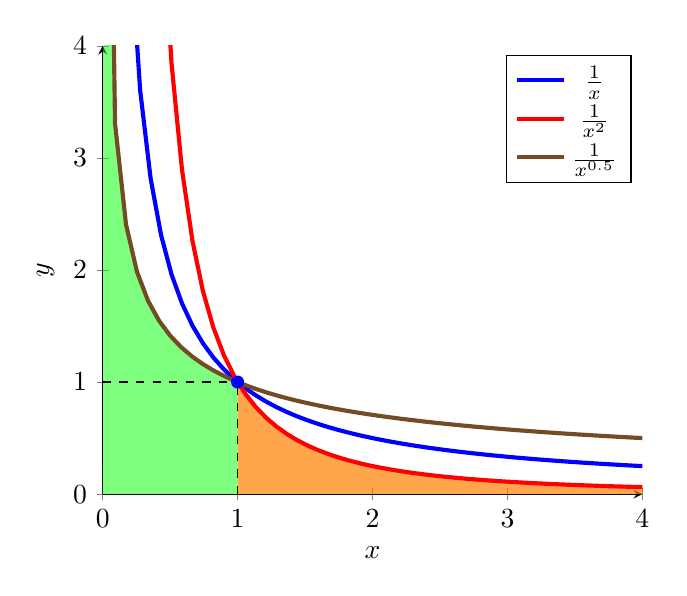
\begin{tikzpicture}
    \begin{axis}[axis x line=bottom, axis y line=left, xmin=0, xlabel={$x$}, ylabel={$y$}, ymin=0, ymax=4]
        \draw[dashed] (1,0) -- (1,1);
        \draw[dashed] (0,1) -- (1,1);
        \addplot+ [name path=A,domain=0.2:4,no markers,line width=1.5pt,samples=50] {1/x};
        \addplot+ [name path=B,domain=0.2:4,no markers,line width=1.5pt,samples=50] {1/(x^2)};
        \addplot+ [name path=C,domain=0.01:4,no markers,line width=1.5pt,samples=50] {1/(x^0.5)};
        \node [fill=blue,circle,scale=0.5] at (1,1) {};
        \path [name path=X] (0,0) -- (4,0);
        \path [name path=Y] (0,0) -- (0,4);
        \addplot [orange,opacity=0.7] fill between [of=B and X,soft clip={domain=1:4}];
        \addplot [green,opacity=0.5] fill between [of=C and X,soft clip={domain=0:1}];
        \legend{$\frac{1}{x}$,$\frac{1}{x^2}$,$\frac{1}{x^{0.5}}$}
    \end{axis}
\end{tikzpicture}

\chapter{多元函数微分学}

\section{多元函数的偏导}

\begin{definition}[多元函数的极限]
    设 $D$ 是 $\mathbb{R}^n$ 上的开集,$x_0=\left(x_1^0,x_2^0,\cdots,x_n^0\right)\in D$ 为一定点,$z=f(\mathbf{x})$ 是定义在 $D\backslash \{x_0\}$ 上的 $n$ 元函数,$A$ 是一个实数。如果对于任意给定的 $\epsilon>0$,存在 $\delta>0$,使得当 $\boldsymbol{x}\in O(\boldsymbol{x}_0,\delta)\backslash\{\boldsymbol{x}_0\}$ 时,成立
    \begin{equation}
        |f(\boldsymbol{x})-A|<\epsilon
    \end{equation}
    则称当 $\boldsymbol{x}$ 趋于 $\boldsymbol{x}_0$ 时 $f$ 收敛,并称 $A$ 为 $f$ 趋于 $\boldsymbol{x}_0$ 时的($n$ 重)极限,记为
    \begin{equation}
        \lim_{\boldsymbol{x}\rightarrow\boldsymbol{x}_0}f(\boldsymbol{x})=A
    \end{equation}
\end{definition}

\begin{definition}[多元函数的连续性]
    设 $D$ 是 $\mathbb{R}^n$ 上的开集,$z=f(\boldsymbol{x})$ 是定义在 $D$ 上的函数,$x_0\in D$ 为一定点。如果
    \begin{equation}
        \lim_{\boldsymbol{x}\rightarrow\boldsymbol{x}_0}f(\boldsymbol{x})=f(\boldsymbol{x}_0)
    \end{equation}
    则称函数在 $f$ 在点 $\boldsymbol{x}_0$ 连续。如果函数 $f$ 在 $D$ 上的每一点连续,就称 $f$ 在 $D$ 上连续,或称 $f$ 是 $D$ 上的连续函数。
\end{definition}

\begin{definition}[偏导数]
    设 $D\subseteq\mathbb{R}^2$ 为开集,
    \begin{equation*}
        z=f(x,y),\quad (x,y)\in D
    \end{equation*}
    是定义在 $D$ 上的二元函数,$(x_0,y_0)\in D$ 为一定点。如果存在极限
    \begin{equation}
        \lim_{\Delta x\rightarrow 0}\frac{f(x_0+\Delta x,y_0)-f(x_0,y_0)}{\Delta x}
    \end{equation}
    那么就称函数 $f$ 在点 $(x_0,y_0)$ 关于 $x$ 可偏导,并称此极限为 $f$ 在点 $(x_0,y_0)$ 关于 $x$ 的偏导数,记为
    \begin{equation}
        \frac{\partial z}{\partial x}(x_0,y_0)
    \end{equation}
\end{definition}

\begin{definition}[全微分]
    设 $D\subseteq\mathbb{R}^2$ 为开集,
    \begin{equation*}
        z=f(x,y),\quad (x,y)\in D
    \end{equation*}
    是定义在 $D$ 上的二元函数,$(x_0,y_0)\in D$ 为一定点。
    若存在只与点 $(x_0,y_0)$ 有关而与 $\Delta x,\Delta y$ 无关的常数 $A$ 和 $B$,使得
    \begin{equation}
        \Delta z=A\Delta x+B\Delta y+o\left(\sqrt[]{(\Delta x)^2+(\Delta y)^2}\right)
    \end{equation}
    则称函数 $f$ 在点 $(x_0,y_0)$ 处是可微的,并称其线性主要部分 $A\Delta x+B\Delta y$ 为 $f$ 在点 $(x_0,y_0)$ 处的全微分,记为 $\diff z(x_0,y_0)$ 或 $\diff f(x_0,y_0)$。
\end{definition}

\begin{theorem}[全微分公式]
    可微必连续,可微必可偏导,有全微分公式
    \begin{equation}
        \diff f(x_0,y_0)=\frac{\partial f}{\partial x}(x_0,y_0)\diff x + \frac{\partial f}{\partial y}(x_0,y_0)\diff y
    \end{equation}
\end{theorem}

\begin{definition}[高阶偏导数]
    设 $z=f(x,y)$ 在区域 $D\subseteq\mathbb{R}^2$ 上具有偏导函数
    \begin{equation}
        \frac{\partial z}{\partial x}=f_x(x,y)\quad \frac{\partial z}{\partial y}=f_y(x,y)
    \end{equation}
    那么在 $D$ 上,如果这两个偏导函数的偏导数也存在,则称它们是 $f(x,y)$ 的二阶偏导数。
    \begin{align*}
        \frac{\partial^2 z}{\partial x^2}&=\frac{\partial}{\partial x}\left(\frac{\partial z}{\partial x}\right) &\frac{\partial^2 z}{\partial x\partial y}&=\frac{\partial}{\partial x}\left(\frac{\partial z}{\partial y}\right)\\
        \frac{\partial^2 z}{\partial y\partial x}&=\frac{\partial}{\partial y}\left(\frac{\partial z}{\partial x}\right)& \frac{\partial^2 z}{\partial y^2}&=\frac{\partial z}{\partial y}\left(\frac{\partial z}{\partial y}\right)
    \end{align*}
    二阶及二阶以上的偏导数统称为高阶偏导数。
\end{definition}

\begin{theorem}[混合偏导数交换]
    如果函数 $z=f(x,y)$ 的两个混合偏导数 $f_{xy}$ 和 $f_{yx}$ 在点 $(x_0,y_0)$ 连续,那么等式
    \begin{equation}
        f_{xy}(x_0,y_0)=f_{yx}(x_0,y_0)
    \end{equation}
\end{theorem}

\begin{definition}[高阶微分]
    设 $z=f(x,y)$ 在区域 $D\subseteq\mathbb{R}^2$ 上具有连续偏导数,那么它是可微的,并且
    \begin{equation}
        \diff z=\frac{\partial z}{\partial x}\diff x+\frac{\partial z}{\partial y}\diff y=\left(\diff x\frac{\partial}{\partial x}+\diff y\frac{\partial}{\partial y}\right)z
    \end{equation}
    若 $z$ 还具有二阶连续偏导数,那么 $\frac{\partial x}{\partial y}$ 也是可微的,从而 $\diff z$ 可微。我们称 $\diff z$ 的微分为 $z$ 的二阶微分
    \marginnote{证明用到了对于自变量 $x$,$\diff^2 x=\diff(\diff x)=0$,$y$ 同理。}
    \begin{equation}
        \diff^2 z=\frac{\partial^2 z}{\partial x^2}\diff x^2+2\frac{\partial^2 z}{\partial x\partial y}\diff x\diff y+\frac{\partial^2 z}{\partial y^2}\diff y^2=\left(\diff x\frac{\partial}{\partial x}+\diff y\frac{\partial}{\partial y}\right)^2z
    \end{equation}
    对 $n$ 元函数 $u=f(x_1,x_2,\cdots,x_n)$ 可同样定义各阶微分,并且成立
    \begin{equation}
        \diff^k u=\left(\diff x_1\frac{\partial}{\partial x_1}+\diff x_2\frac{\partial}{\partial x_2}+\cdots+\diff x_n\frac{\partial}{\partial x_n}\right)^k u
    \end{equation}
\end{definition}

\section{向量值函数}

\begin{definition}[向量值函数]
    设 $D$ 是 $\mathbb{R}^n$ 上的点集,$D$ 到 $\mathbb{R}^m$ 的映射
    \begin{equation}
        \begin{aligned}
            \boldsymbol{f}:D&\rightarrow\mathbb{R}^m\\
            \boldsymbol{x}=(x_1,x_2,\cdots,x_n)&\mapsto \boldsymbol{y}=(y_1,y_2,\cdots,y_m)
        \end{aligned}
    \end{equation}
    称为 $n$ 元 $m$ 维向量值函数(或多元函数组),记为 $\boldsymbol{y}=\boldsymbol{f}(\boldsymbol{x})$。
\end{definition}

\begin{definition}[向量值函数的导数]
    若 $\boldsymbol{f}$ 的每一个分量函数 $f_i(x_1,x_2,\cdots,x_n)(i=1,2,\cdots,m)$ 都在点 $\boldsymbol{x}^0=(x_1^0,x_2^0,\cdots,x_n^0)^\top\in D$ 可偏导,就称向量值函数 $\boldsymbol{f}$ 在 $\boldsymbol{x}^0$ 点可导,并称矩阵
    \begin{equation}
        \boldsymbol{f}^\prime(\boldsymbol{x}^0)=\left(\frac{\partial f_i}{\partial x_j}(\boldsymbol{x}^0)\right)_{m\times n}=\begin{pmatrix}
            \frac{\partial f_1}{\partial x_1} & \frac{\partial f_1}{\partial x_2} & \cdots & \frac{\partial f_1}{\partial x_n} \\
            \frac{\partial f_2}{\partial x_1} & \frac{\partial f_2}{\partial x_2} & \cdots & \frac{\partial f_2}{\partial x_n} \\
            \vdots & \vdots & \ddots & \vdots \\
            \frac{\partial f_m}{\partial x_1} & \frac{\partial f_m}{\partial x_2} & \cdots & \frac{\partial f_m}{\partial x_n} \\
        \end{pmatrix}\left(\boldsymbol{x}^0\right)
    \end{equation}
    为向量值函数 $\boldsymbol{f}$ 在 $\boldsymbol{x}^0$ 点的导数或 Jacobi 矩阵。
\end{definition}

\begin{theorem}[向量值函数的微分公式]
    向量值函数 $\boldsymbol{f}$ 在 $\boldsymbol{x}^0$ 点可微的充分必要条件是它的坐标分量函数 $f_i(x_1,x_2,\cdots,x_n)(i=1,2,\cdots,m)$ 都在 $\boldsymbol{x}^0$ 点可微。此时成立微分公式
    \begin{equation}
        \diff\boldsymbol{y}=\boldsymbol{f}^\prime(\boldsymbol{x}^0)\diff \boldsymbol{x}
    \end{equation}
\end{theorem}

\section{复合函数求导}

\begin{definition}[多元复合函数链式规则]
    设 $\boldsymbol{g}$ 在 $(u_0,v_0)\in D_g$ 点可导,如果 $f$ 在 $(x_0,y_0)$ 点可微,那么
    \marginnote{简记为$(f\circ \boldsymbol{g})^\prime(x_0)=f^\prime(y_0)\boldsymbol{g}^\prime(\boldsymbol{x}_0)$}
    \begin{equation}
        \begin{pmatrix}
            \frac{\partial z}{\partial u} & \frac{\partial z}{\partial v}
        \end{pmatrix} = \begin{pmatrix}
            \frac{\partial z}{\partial x} & \frac{\partial z}{\partial y}
        \end{pmatrix}
        \begin{pmatrix}
            \frac{\partial x}{\partial u} & \frac{\partial x}{\partial v} \\
            \frac{\partial y}{\partial u} & \frac{\partial y}{\partial v}
        \end{pmatrix}
    \end{equation}
\end{definition}

\begin{theorem}[一阶全微分的形式不变性]
    当 $x,y$ 为中间变量时
    \begin{equation}
        \begin{aligned}
            x &= x(u,v) \\
            y &= y(u,v)
        \end{aligned}
    \end{equation}
    则
    \marginnote{
        也可以理解为
        $\begin{aligned}\diff z&=(f\circ\boldsymbol{g})^\prime(\boldsymbol{x})\diff x\\&=f^\prime(\boldsymbol{y})\boldsymbol{g}^\prime(\boldsymbol{x})\diff\boldsymbol{x}\\&=f^\prime(\boldsymbol{y})(\boldsymbol{g}^\prime(\boldsymbol{x})\diff\boldsymbol{x})\\&=f^\prime(\boldsymbol{y})\diff\boldsymbol{y}\end{aligned}$
    }
    \begin{equation}
        \begin{aligned}
            \diff z &= \begin{pmatrix}
                \frac{\partial z}{\partial u} & \frac{\partial z}{\partial v}
            \end{pmatrix}
            \begin{pmatrix}
                \diff u\\
                \diff v
            \end{pmatrix}\\
            &=\begin{pmatrix}
                \frac{\partial z}{\partial x} & \frac{\partial z}{\partial y}
            \end{pmatrix}
            \begin{pmatrix}
                \frac{\partial x}{\partial u} & \frac{\partial x}{\partial v} \\
                \frac{\partial y}{\partial u} & \frac{\partial y}{\partial v}
            \end{pmatrix}
            \begin{pmatrix}
                \diff u\\
                \diff v
            \end{pmatrix}\\
            &=\begin{pmatrix}
                \frac{\partial z}{\partial x} & \frac{\partial z}{\partial y}
            \end{pmatrix}
            \begin{pmatrix}
                \diff x\\
                \diff y
            \end{pmatrix}
        \end{aligned}
    \end{equation}
    \marginnote{全微分的形式不变性在高阶微分时是不成立的。}
    无论 $x,y$ 是自变量,还是中间变量,一阶微分具有相同的形式,这就是一阶全微分的形式不变性。
\end{theorem}

\section{隐函数}

\begin{theorem}[一元隐函数存在定理]
    若二元函数 $F(x,y)$ 满足条件:
    \begin{enumerate}
        \item $F(x_0,y_0)=0$
        \item 在闭矩形 $D=\{(x,y)||x-x_0|\leq a,|y-y_0|\leq b\}$ 上,$F(x,y)$ 连续,且具有连续偏导数
        \item $F_y(x_0,y_0)\neq 0$
    \end{enumerate}
    那么
    \begin{enumerate}
        \item 在点 $(x_0,y_0)$ 附近可以从函数方程
        \begin{equation*}
            F(x,y)=0
        \end{equation*}
        唯一确定隐函数
        \begin{equation}
            y=f(x), x\in O(x_0,\rho)
        \end{equation}
        它满足 $F(x,f(x))=0$,以及 $y_0=f(x_0)$
        \item 隐函数 $y=f(x)$ 在 $x\in O(x_0,\rho)$ 上连续
        \item 隐函数 $y=f(x)$ 在 $x\in O(x_0,\rho)$ 上具有连续的导数,且
        \begin{equation}
            \frac{\diff y}{\diff x}=-\frac{F_x(x,y)}{F_y(x,y)}
        \end{equation}
    \end{enumerate}
\end{theorem}

\begin{theorem}[多元隐函数存在定理]
    (从略)
    \begin{equation}
        \frac{\partial y}{\partial x_i}=-\frac{F_{x_i}(x_1,x_2,\cdots,x_n,y)}{F_y(x_1,x_2,\cdots,x_n,y)},\quad i=1,2,\cdots,n
    \end{equation}
\end{theorem}

\begin{theorem}[多元向量值隐函数存在定理]
    设函数 $F(x,y,u,v)$ 和 $G(x,y,u,v)$ 满足条件:
    \begin{enumerate}
        \item $F(x_0,y_0,u_0,v_0)=0,G(x_0,y_0,u_0,v_0)=0$
        \item 在闭长方体
        \begin{equation*}
            D=\{(x,y,u,v)||x-x_0|\leq a,|y-y_0|\leq b, |u-u_0|\leq c,|v-v_0|\leq d\}
        \end{equation*}
        上,函数 $F,G$ 连续,且具有连续偏导数
        \item 在 $(x_0,y_0,u_0,v_0)$ 点,行列式
        \begin{equation}
            \frac{\partial (F,G)}{\partial (u,v)}=\mqty|F_u & F_v \\G_u & G_v|\neq 0
        \end{equation}
    \end{enumerate}
    那么
    \begin{enumerate}
        \item 在点 $(x_0,y_0,u_0,v_0)$ 附近可以从函数方程组
        \begin{equation}
            \begin{cases}
                F(x,y,u,v)=0,\\
                G(x,y,u,v)=0
            \end{cases}
        \end{equation}
        唯一确定向量值隐函数
        \begin{equation}
            \mqty(u\\ v)=\mqty(f(x,y)\\ g(x,y)), (x,y)\in O((x_0,y_0),\rho)
        \end{equation}
        它满足$\begin{cases}
                F(x,y,f(x,y),g(x,y))=0\\
                G(x,y,f(x,y),g(x,y))=0
            \end{cases}$
        以及 $u_0=f(x_0,y_0),v_0=g(x_0,y_0)$。
        \item 这个向量值隐函数在 $O((x_0,y_0),\rho)$ 上连续
        \item 这个向量值隐函数在 $O((x_0,y_0),\rho)$ 上具有连续的导数,且
        \begin{equation}
            \mqty(\frac{\partial u}{\partial x} & \frac{\partial u}{\partial y}\\
            \frac{\partial v}{\partial x} & \frac{\partial v}{\partial y})=
            -\mqty(F_u & F_v\\ G_u & G_v)^{-1}\mqty(F_x & F_y\\ G_x & G_y)
        \end{equation}
    \end{enumerate}
\end{theorem}

\begin{theorem}[多函数多元向量值隐函数存在定理]
    (从略)
    \begin{equation}
        \begin{pmatrix}
            \frac{\partial y_1}{\partial x_1} & \frac{\partial y_1}{\partial x_2} & \cdots & \frac{\partial y_1}{\partial x_n} \\
            \frac{\partial y_2}{\partial x_1} & \frac{\partial y_2}{\partial x_2} & \cdots & \frac{\partial y_2}{\partial x_n} \\
            \vdots & \vdots & \ddots & \vdots \\
            \frac{\partial y_m}{\partial x_1} & \frac{\partial y_m}{\partial x_2} & \cdots & \frac{\partial y_m}{\partial x_n}
        \end{pmatrix}=
        -\begin{pmatrix}
            \frac{\partial F_1}{\partial y_1} & \frac{\partial F_1}{\partial y_2} & \cdots & \frac{\partial F_1}{\partial y_n} \\
            \frac{\partial F_2}{\partial y_1} & \frac{\partial F_2}{\partial y_2} & \cdots & \frac{\partial F_2}{\partial y_n} \\
            \vdots & \vdots & \ddots & \vdots \\
            \frac{\partial F_m}{\partial y_1} & \frac{\partial F_m}{\partial y_2} & \cdots & \frac{\partial F_m}{\partial y_n} \\
        \end{pmatrix}^{-1}
        \begin{pmatrix}
            \frac{\partial F_1}{\partial x_1} & \frac{\partial F_1}{\partial x_2} & \cdots & \frac{\partial F_1}{\partial x_n} \\
            \frac{\partial F_2}{\partial x_1} & \frac{\partial F_2}{\partial x_2} & \cdots & \frac{\partial F_2}{\partial x_n} \\
            \vdots & \vdots & \ddots & \vdots \\
            \frac{\partial F_m}{\partial x_1} & \frac{\partial F_m}{\partial x_2} & \cdots & \frac{\partial F_m}{\partial x_n} \\
        \end{pmatrix}
    \end{equation}
\end{theorem}

\begin{theorem}[逆映射定理]
    设 $\boldsymbol{P}_0=(u_0,v_0)\in D$,$x_0=x(u_0,v_0),y_0=y(u_0,v_0),\boldsymbol{P}_0^\prime =(x_0,y_0)$,且 $f$ 在 $D$ 上具有连续导数。如果在 $\boldsymbol{P}_0$ 点处 $\boldsymbol{f}$ 的 Jacobi 行列式
    \begin{equation}
        \frac{\partial (x,y)}{\partial (u,v)}\neq 0
    \end{equation}
    那么存在 $\boldsymbol{P}_0^\prime$ 的一个邻域 $O(\boldsymbol{P}_0^\prime,\rho)$,在这个邻域上存在 $\boldsymbol{f}$ 的具有连续导数的逆映射 $\boldsymbol{g}$:
    \begin{equation}
        \begin{cases}
            u=u(x,y)\\
            v=v(x,y)
        \end{cases}
        (x,y)\in O(\boldsymbol{P}_0^\prime,\rho)
    \end{equation}
    满足
    \begin{enumerate}
        \item $u_0=u(x_0,y_0),v_0=v(x_0,y_0)$
        \item \begin{equation}
            \begin{aligned}
                \frac{\partial u}{\partial x}&=\frac{\frac{\partial y}{\partial v}}{\frac{\partial (x,y)}{\partial (u,v)}} & \frac{\partial u}{\partial y}&=-\frac{\frac{\partial x}{\partial v}}{\frac{\partial (x,y)}{\partial (u,v)}}\\
                \frac{\partial v}{\partial x}&=\frac{\frac{\partial y}{\partial u}}{\frac{\partial (x,y)}{\partial (u,v)}} & \frac{\partial v}{\partial y}&=-\frac{\frac{\partial x}{\partial u}}{\frac{\partial (x,y)}{\partial (u,v)}}
            \end{aligned}
        \end{equation}
    \end{enumerate}
\end{theorem}

\section{多元函数的中值定理与Taylor公式}

\begin{theorem}[多元函数的中值定理]
    设二元函数 $f(x,y)$ 在凸区域 $D\subseteq \mathbb{R}^2$ 上可微,则对于 $D$ 内任意两点 $(x_0,y_0)$ 和 $(x_0+\Delta x,y_0+\Delta y)$,至少存在一个 $\theta(0<\theta<1)$,使得
    \begin{equation}
        \begin{aligned}
            &f(x_0+\Delta x,y_0+\Delta y)-f(x_0,y_0) \\            
           =&f_x(x_0+\theta\Delta x,y_0+\theta\Delta y)\Delta x+f_y(x_0+\theta\Delta x,y_0+\theta\Delta y)\Delta y
        \end{aligned}
    \end{equation}
\end{theorem}

\begin{theorem}[多元函数的Taylor公式]
    设函数 $f(x,y)$ 在点 $(x_0,y_0)$ 的邻域 $U=O((x_0,y_0),r)$ 上具有 $k+1$ 阶连续偏导数,那么对于 $U$ 内每一点 $(x_0+\Delta x,y_0+\Delta y)$ 都成立
    \begin{equation}
        \begin{aligned}
            &f(x_0+\Delta x,y_0+\Delta y)\\
           =&f(x_0,y_0)+\left(\Delta x\frac{\partial}{\partial x}+\Delta y\frac{\partial}{\partial y}\right)f(x_0,y_0)+\frac{1}{2!}\left(\Delta x\frac{\partial}{\partial x}+\Delta y\frac{\partial}{\partial y}\right)^2f(x_0,y_0)\\
           &+\cdots+\frac{1}{k!}\left(\Delta x\frac{\partial}{\partial x}+\Delta y\frac{\partial}{\partial y}\right)^k f(x_0,y_0)+R_k
        \end{aligned}
    \end{equation}
    其中
    \begin{equation}
        R_k=\frac{1}{(k+1)!}\left(\Delta x\frac{\partial}{\partial x}+\Delta \frac{\partial}{\partial y}\right)^{k+1}f(x_0+\theta\Delta x,y_0+\theta\Delta y) \quad (0<\theta<1)
    \end{equation}
\end{theorem}

\section{无条件极值}

\begin{definition}[无条件极值]
    设 $D\in\mathbb{R}^n$ 为开区域,$f(\boldsymbol{x})$ 为定义在 $D$ 上的函数,$\boldsymbol{x}_0=(x_1^0,x_2^0,\cdots,x_n^0)\in D$。若存在 $\boldsymbol{x}_0$ 的邻域 $O(\boldsymbol{x}_0,r)$,使得
    \begin{equation}
        f(\boldsymbol{x}_0)\geq f(\boldsymbol{x}),\quad\boldsymbol{x}\in O(\boldsymbol{x}_0,r)
    \end{equation}
    则称 $\boldsymbol{x}_0$ 为 $f$ 的极大值点。极小值点可以对应定义。
\end{definition}

\begin{theorem}[无条件极值必要条件]
    设 $\boldsymbol{x}_0$ 为函数 $f$ 的极值点,且 $f$ 在 $\boldsymbol{x}_0$ 点可偏导,则 $f$ 在 $\boldsymbol{x}_0$ 点的各个一阶偏导数都为零,即
    \begin{equation}
        f_{x_1}(\boldsymbol{x}_0)=f_{x_2}(\boldsymbol{x}_0)=\cdots=f_{x_n}(\boldsymbol{x}_0)=0
    \end{equation}
\end{theorem}

\begin{theorem}[无条件极值充分条件]
    设 $(x_0,y_0)$ 为 $f$ 的驻点,$f$ 在 $(x_0,y_0)$ 附近具有二阶连续偏导数。
    \marginpar{Hesse矩阵}
    \begin{equation}
        H=\begin{pmatrix}
            f_{xx}(x_0,y_0) & f_{xy}(x_0,y_0) \\
            f_{xy}(x_0,y_0) & f_{yy}(x_0,y_0)
        \end{pmatrix}
    \end{equation}
    若 $|H|>0$,且 $f_{xx}(x_0,y_0)>0$ 时 $f(x_0,y_0)$ 为极小值;若 $|H|>0$,且 $f_{xx}(x_0,y_0)<0$ 时 $f(x_0,y_0)$ 为极大值;若 $|H|<0$,$f(x_0,y_0)$ 不是极值。\marginnote{$|H|=0$ 时,判别法失效,可以考虑不等式。}
\end{theorem}

\begin{theorem}[无条件极值充分条件多元推广]
    设 $n$ 元函数 $f(\boldsymbol{x})$ 在 $\boldsymbol{x}_0=(x_1^0,x_2^0,\cdots,x_n^0)$ 附近具有二阶连续偏导数,且 $\boldsymbol{x}_0$ 为 $f(\boldsymbol{x})$ 的驻点。那么当二次型
    \begin{equation}
        g(\zeta)=\sum_{i,j=1}^n f_{x_ix_j}(\boldsymbol{x}_0)\zeta_i\zeta_j
    \end{equation}
    正定时,$f(\boldsymbol{x}_0)$ 为极小值;当 $g(\zeta)$ 负定时,$f(\boldsymbol{x}_0)$ 为极大值;当 $g(\zeta)$ 不定时,$f(\boldsymbol{x}_0)$ 不是极值。

    记 $h_{ij}=f_{x_ix_j}(\boldsymbol{x}_0)$,
    \begin{equation}
        \boldsymbol{H}_k=\begin{pmatrix}
            h_{11} & h_{12} & \cdots & h_{1n} \\
            h_{21} & h_{22} & \cdots & h_{2n} \\
            \vdots & \vdots & \ddots & \vdots \\
            h_{k1} & h_{k2} & \cdots & h_{kk}
        \end{pmatrix}
    \end{equation}
    为 $f$ 的 $k$ 阶 Hesse 矩阵。若 $|\boldsymbol{H}_k|>0(k=1,2,\cdots,n)$,则二次型是正定的,此时为极小值;若 $(-1)^k|\boldsymbol{H}_k|>0(k=1,2,\cdots,n)$,则二次型为负定的,此时为极大值。
\end{theorem}

\section{有条件极值}

\begin{theorem}[Lagrange 乘数法]
    考虑目标函数 $f(x_1,x_2,\cdots,x_n)$ 在 $m$ 个约束条件
    \begin{equation}
        g_i(x_1,x_2,\cdots,x_n)=0\quad (i=1,2,\cdots,m; m<n)
    \end{equation}
    下的极值。这里 $f,g_i(i=1,2,\cdots,m)$ 具有连续偏导数,且 Jacobi 矩阵在满足约束条件的点处是满秩的。构造 Lagrange 函数
    \begin{equation}
        L(x_1,x_2,\cdots,x_n,\lambda_1,\lambda_2,\cdots,\lambda_m)=f(x_1,x_2,\cdots,x_n)-\sum_{i=1}^m\lambda_ig_i(x_1,x_2,\cdots,x_n)
    \end{equation}
    条件极值点就在方程组
    \begin{equation}
        \begin{cases}
            \frac{\partial L}{\partial x_k}=\frac{\partial f}{\partial x_k}-\sum_{i=1}^m\lambda_i\frac{\partial g_i}{\partial x_k}=0\\
            g_l=0
        \end{cases}
        (k=1,2,\cdots,n;l=1,2,\cdots,m)
    \end{equation}
    的所有解 $(x_1,x_2,\cdots,x_n,\lambda_1,\lambda_2,\cdots,\lambda_m)$ 所对应的点 $(x_1,x_2,\cdots,x_n)$ 中。
\end{theorem}

\chapter{二重积分}

\begin{definition}[二重积分]
    设 $D$ 为 $\mathbb{R}^2$ 上的零边界闭区域,函数 $z=f(x,y)$ 在 $D$ 上有界。将 $D$ 用曲线网分成 $n$ 个小区域 $\Delta D_1,\Delta D_2,\cdots,\Delta D_n$(它称为 $D$ 的一个划分),并记所有的一区域 $\Delta D_i$ 的最大直径为 $\lambda$,即
    \begin{equation}
        \lambda = \max_{1\leq i\leq n}\{\textnormal{diam}\Delta D_i\}
    \end{equation}
    在每个 $\Delta D_i$ 上任取一点 $(\xi_i, \eta_i)$,记 $\Delta\sigma_i$ 为 $\Delta D_i$ 的面积,若和式
    \begin{equation}
        \lim_{\lambda\rightarrow 0}\sum_{i=1}^n f(\xi_i,\eta_i)\Delta\sigma_i
    \end{equation}
    存在且与区域的分法和点 $(\xi_i,\eta_i)$ 的取法无关,则称 $f(x,y)$ 在 $D$ 上可积,并称此极限为 $f(x,y)$ 在 $D$ 上的二重积分,记为
    \begin{equation}
        \iint_D f(x,y)\diff\sigma
    \end{equation}
\end{definition}

\begin{proposition}[重积分的性质]
    设 $f$ 和 $g$ 都在区域 $\Omega$ 上可积。
    \begin{description}
        \item[线性性]  $\alpha,\beta$ 为常数,则 $\alpha f+\beta g$ 在 $\Omega$ 上可积,
        \begin{equation}
            \int_\Omega (\alpha f+\beta g)\diff V=\alpha\int_\Omega f\diff V+\beta\int_\Omega g\diff V
        \end{equation}
        \item[区域可加性] 设区域 $\Omega$ 被分成两个内点不相交的区域 $\Omega_1$ 和 $\Omega_2$,如果 $f$ 在 $\Omega$ 上可积。
        \begin{equation}
            \int_\Omega f\diff V=\int_{\Omega_1} f\diff V+\int_{\Omega_2} f\diff V
        \end{equation}
        \item[保序性] 满足 $f\leq g$,则成立不等式
        \begin{equation}
            \int_\Omega f\diff V\leq \int_\Omega g\diff V
        \end{equation}
        \item \begin{equation}
            \begin{aligned}
                M=\sup_\Omega f,\quad m=\inf_\Omega f\\
                \Rightarrow mV\leq \int_\Omega f\diff V\leq MV
            \end{aligned}
        \end{equation}
        \item[绝对可积性] $|f|$ 也在 $\Omega$ 上可积,
        \begin{equation}
            \left|\int_\Omega f\diff V\right|\leq\int_\Omega |f|\diff V
        \end{equation}
        \item[乘积可积性] $f\cdot g$ 也在 $\Omega$ 上可积。
        \item[积分中值定理] $g$ 在 $\Omega$ 上不变号。$M=\sup_\Omega f,m=\inf_\Omega f$,则存在常数 $\mu\in[m,M]$,使得
        \begin{equation}
            \int_\Omega f\cdot g\diff V=\mu\int_\Omega g\diff V
        \end{equation}
        特别地,如果 $f$ 在 $\Omega$ 上连续,则存在 $\xi\in\Omega$,使得
        \begin{equation}
            \int_\Omega f\cdot g\diff V=f(\xi)\int_\Omega g\diff V
        \end{equation}
    \end{description}
\end{proposition}

\begin{theorem}[矩形区域上的二重积分]
    设二元函数 $f(x,y)$ 在闭矩形 $D=[a,b]\times[c,d]$ 上可积。
    \begin{equation}
        \iint_D f(x,y)\diff x\diff y=\int_a^b\left(\int_c^d f(x,y)\diff y\right)\diff x=\int_a^b\diff x\int_c^d f(x,y)\diff y
    \end{equation}
\end{theorem}

\begin{theorem}[二重积分变量代换公式]
    设 $U$ 为 $uv$ 平面上的开集,$V$ 是 $xy$ 平面上的开集,映射
    \begin{equation}
        T: x=x(u,v),\quad y=y(u,v)
    \end{equation}
    是 $U$ 到 $V$ 的一一对应。
    % 它的逆变换记为 $T^{-1}:u=u(x,y),v=v(x,y)$。
    假设 $x=x(u,v),y=y(u,v)$ 具有连续偏导数,且有 $\frac{\partial (x,y)}{\partial (u,v)}\neq 0$,则有连续性可知 \marginpar{Jacobi 矩阵}$\frac{\partial (x,y)}{\partial(u,v)}$ 在 $U$ 上不变号。则对于任意具有分段光滑边界的有界闭区域 $D$,
    \begin{equation}
        \iint_{T(D)}f(x,y)\diff x\diff y=\iint_D f(x(u,v),y(u,v))\left|\frac{\partial(x,y)}{\partial(u,v)}\right|\diff u\diff v
    \end{equation}
\end{theorem}

\begin{definition}[二重积分的应用]
    \begin{description}
        \item[面积] \begin{equation}
            \iint_\Omega \diff x\diff y=\iint_\Omega 1\diff x\diff y=\Omega\text{的面积}
        \end{equation}
        \item[曲顶柱体体积] 曲顶为 $z=z(x,y),(x,y)\in D_{xy}$ 的柱体体积
        \begin{equation}
            V=\iint_{D_{xy}}|z(x,y)|\diff\sigma
        \end{equation}
        \item[总质量] \begin{equation}
            m=\iint_D \rho(x,y)\diff\sigma
        \end{equation}
        \item[重心坐标] 对于平面薄片,面密度为 $\rho(x,y)$,$D$ 是薄片所占的平面区域,则计算重心 $(\bar{x},\bar{y})$ 的公式为
        \begin{equation}
            \bar{x}=\frac{\iint_D x\rho(x,y)\diff\sigma}{\iint_D\rho(x,y)\diff\sigma},\bar{y}=\frac{\iint_D y\rho(x,y)\diff\sigma}{\iint_D\rho(x,y)\diff\sigma}
        \end{equation}
        \item[转动惯量] 对于平面薄片,面密度为 $\rho(x,y)$,$D$ 是薄片所占的平面区域,则计算该薄片对 $x$ 轴、$y$ 轴和原点 $O$ 的转动惯量
        \begin{equation}
            \begin{aligned}
                I_x&=\iint_D y^2\rho(x,y)\diff\sigma\\
                I_y&=\iint_D x^2\rho(x,y)\diff\sigma\\
                I_O&=\iint_D (x^2+y^2)\rho(x,y)\diff\sigma
            \end{aligned}
        \end{equation}
    \end{description}
\end{definition}

\begin{theorem}[Possion 积分]
    \begin{equation}
        \int_0^{+\infty}\e^{-x^2}\diff x=\frac{\sqrt[]{\pi}}{2}
    \end{equation}
    方法是化为二维累次积分\marginpar{类似的还有\begin{align*}
        &\int_{0}^\infty\frac{\sin x}{x}\diff x\\
        &=\int_{0}^\infty\frac{\sin x}{x}\int_{0}^{+\infty}\e^{-u}\diff u\diff x
    \end{align*}}
    \begin{equation}
        \pi=\iint_{\mathbb{R}^2}\e^{-(x^2+y^2)}\diff x\diff y=\int_{-\infty}^{+\infty}\e^{-x^2}\diff x\int_{-\infty}^{+\infty}\e^{-y^2}\diff y=\left(\int_{-\infty}^{+\infty}\e^{-x^2}\diff x\right)^2
    \end{equation}
\end{theorem}

\chapter{微分方程}

\begin{definition}[微分方程]
    凡表示未知函数、未知函数的导数与自变量之间的关系的方程,叫做微分方程,所出现的未知函数的最高阶导数的阶数,叫做微分方程的阶。如果微分方程的解含有任意常数,且任意常数的个数与微分方程的阶数\underline{相同},这样的解叫做微分方程的通解。通过初值条件,确定了通解中的任意常数以后,就得到微分方程的特解。
\end{definition}

\begin{definition}[可分离变量的微分方程]
    如果一个一阶微分方程能写成
    \begin{equation}
        g(y)\diff y=f(x)\diff x
    \end{equation}
    的形式,那么原方程就是可分离变量的微分方程。
    \begin{equation}
        y^\prime=f(x)\cdot g(y)\Rightarrow \frac{\diff y}{g(y)}=f(x)\diff x\Rightarrow \int \frac{\diff y}{g(y)} = \int f(x)\diff x
    \end{equation}
    \begin{equation}
        y^\prime=f(ax+by+c)\xrightarrow[u^\prime=a+bf(u)]{u=ax+by+c}\frac{\diff u}{a+bf(u)}=\diff x
    \end{equation}
\end{definition}

\begin{definition}[齐次方程]
    如果一阶微分方程可化成
    \begin{equation}
        \frac{\diff y}{\diff x}=\varphi\left(\frac{y}{x}\right)
    \end{equation}
    令
    \begin{equation}
        u=\frac{y}{x}
    \end{equation}
    则
    \begin{equation}
        u+x\frac{\diff u}{\diff x}=\varphi (u)
    \end{equation}
\end{definition}

\begin{definition}[一阶线性微分方程]
    方程
    \begin{equation}
        \frac{\diff y}{\diff x}+P(x)y=Q(x)
    \end{equation}
    叫做一阶线性微分方程,如果 $Q(x)\equiv 0$,那么它就是齐次的;否则就是非齐次的。

    齐次的通解
    \begin{equation}
        y=C\e^{-\int P(x)\diff x}
    \end{equation}

    非齐次的通解
    \marginpar{等式两边同乘 $e^{\int P(x)\diff x}$}
    \begin{equation}
        y=\e^{-\int P(x)\diff x}\left(\int Q(x)\e^{\int P(x)\diff x}\diff x+C\right)
    \end{equation}
\end{definition}

\begin{definition}[伯努利方程]
    方程
    \begin{equation}
        \frac{\diff y}{\diff x}+P(x)y=Q(x)y^n (n\neq 0,1)
    \end{equation}
    叫做伯努利方程。
    令
    \begin{align}
        z&=y^{1-n}\\
        \frac{\diff z}{\diff x}&=(1-n)y^{-n}\frac{\diff y}{\diff x}
    \end{align}
    则
    \begin{equation}
        \frac{\diff z}{\diff x}+(1-n)P(x)z=(1-n)Q(x)
    \end{equation}
\end{definition}

\begin{definition}[可降阶的高阶微分方程]
    \begin{align}
        y^{(n)}=f(x) &\Rightarrow y^{(n-1)}=\int f(x)\diff x+C_1\\
        y^{\prime\prime}=f(x,y^\prime) & \xrightarrow[y^{\prime\prime}=p^\prime]{y^\prime = p} p^\prime = f(x,p)\\
        y^{\prime\prime}=f(y,y^\prime)&\xrightarrow[y^{\prime\prime}=\frac{\diff p}{\diff y}\frac{\diff y}{\diff x}=p\frac{\diff p}{\diff y}]{y^\prime=p} p\frac{\diff p}{\diff y}=f(y,p)
    \end{align}
\end{definition}

\begin{definition}[二阶齐次线性方程]
    \begin{equation}
        y^{\prime\prime}+P(x)y^\prime+Q(x)y=0
    \end{equation}
    \begin{enumerate}
        \item 如果函数 $y_1(x)$ 与 $y_2(x)$ 是方程的两个解,那么 $y=C_1y_1(x)+C_2y_2(x)$ 也是解,其中 $C_1,C_2$ 是任意常数。
        \item 如果 $y_1(x), y_2(x)$ 是方程的两个线性无关的解,那么 $y=C_1y_1(x)+C_2y_2(x)$ 就是方程的通解。
    \end{enumerate}
\end{definition}

\begin{definition}[二阶非齐次线性方程]
    \begin{equation}
        y^{\prime\prime}+P(x)y^\prime+Q(x)y=f(x)
    \end{equation}
    \begin{enumerate}
        \item 设 $y^*(x)$ 是一个特解,$Y(x)$ 是对应齐次方程的通解,则
        \begin{equation}
            y=Y(x)+y^*(x)
        \end{equation}
        是其通解。
        \item 若 $f(x)=f_1(x)+f_2(x)$,而 $y_1^*(x)$ 和 $y_2^*(x)$ 分别是对应非齐次方程的特解,则 $y_1^*(x)+y_2^*(x)$ 是原方程的特解。
    \end{enumerate}
\end{definition}

\begin{definition}[二阶常系数齐次线性微分方程]
    \begin{equation}
        y^{\prime\prime}+py^\prime+qy=0
    \end{equation}
    如果 $p,q$ 均为常数,称为二阶常系数齐次线性微分方程(否则称为二阶变系数齐次线性微分方程)。
    讨论其特征方程
    \begin{equation}
        r^2+pr+q=0
    \end{equation}
    \begin{align}
        r_1\neq r_2 && y&=C_1\e^{r_1x}+C_2\e^{r_2x}\\
        r_1=r_2 && y&=(C_1+C_2x)\e^{r_1x}\\
        r_1=\alpha+\beta\textnormal{i},r_2=\alpha-\beta\textnormal{i}(\beta\neq 0) && y&=\e^{\alpha x}(C_1\cos\beta x+C_2\sin\beta x)
    \end{align}
\end{definition}

\begin{definition}[二阶常系数非齐次线性微分方程]
    \begin{equation}
        y^{\prime\prime}+py^\prime+qy=f(x)
    \end{equation}
    其中 $p,q$ 为常数,称为二阶常系数非齐次线性微分方程。求特解 $y^*$。
    \begin{enumerate}
        \item $f(x)=\e^{\lambda x}P_m(x)$,$\lambda$ 是常数,$P_m(x)$ 是 $x$ 的一个 $m$ 次多项式。特解为 
        \begin{equation}
            y^*=x^kR_m(x)\e^{\lambda x}
        \end{equation}
        而 $k$ 按 $\lambda$ 不是特征方程的根、是其单根、是其重根分别取 0,1,2。
        \item $f(x)=\e^{\lambda x}[P_l(x)\cos\omega x+Q_n(x)\sin\omega x]$,其中 $\lambda,\omega\neq 0$ 是常数,$P_l(x),Q_n(x)$ 仅有一个可为零。
        则 $f(x)=P(x)\e^{\lambda+\omega\textnormal{i}x}+\overline{P}(x)\e^{(\lambda-\omega\textnormal{i})x}$,则特解
        \begin{equation}
            y^*=x^k\e^{\lambda x}[R_m^{(1)}(x)\cos\omega x+R_m^{(2)}(x)\sin\omega x]
        \end{equation}
        其中 $R_m^{(1)}(x),R_m^{(2)}(x)$ 是 $m=\max\{l,n\}$ 次多项式。而 $k$ 按 $\lambda+\textnormal{i}\omega$ 不是特征方程的根或是特征方程的单根依次取 0 或 1。
    \end{enumerate}
\end{definition}

\begin{definition}[欧拉方程]
    \begin{equation}
        x^ny^{(n)}+p_1x^{n-1}y^{(n-1)}+\cdots+p_{n-1}xy^{\prime}+p_ny=f(x)
    \end{equation}
    其中 $p_i$ 为常数,称为欧拉方程。
    令 $t=\ln x$,则
    \begin{equation}
        x^ky^{(k)}=\frac{\diff}{\diff t}\left(\frac{\diff}{\diff t}-1\right)\cdots\left(\frac{\diff}{\diff t}-k+1\right)y
    \end{equation}
    转化为以 $t$ 为自变量的常系数微分方程。
\end{definition}

\begin{definition}[$n$ 阶常系数齐次线性微分方程]
    \begin{equation}
        y^{(n)}+p_1y^{(n-1)}+p_2y^{(n-2)}+\cdots+p_{n-1}y^\prime+p_ny=0
    \end{equation}
    其中 $p_1,p_2,\cdots,p_{n-1},p_n$ 都是常数。
    记
    \begin{equation}
        L(D)=D^n+p_1D^{n-1}+\cdots+p_{n-1}D+p_n
    \end{equation}
    叫做微分算子 $D$ 的 $n$ 次多项式。
    \begin{align}
        r &\in\mathbb{R} (1)&& C\e^{rx}\\
        r_{1,2} (1)&=\alpha\pm\beta\textnormal{i} && \e^{\alpha x}(C_1\cos\beta x+C_2\sin\beta x)\\
        r &\in\mathbb{R} (k)&& \e^{rx}(C_1+C_2x+\cdots+C_kx^{k-1})\\
        r_{1,2} (k)&=\alpha\pm\beta\textnormal{i} && \e^{\alpha x}[(C_1+C_2x+\cdots+C_kx^{k-1})\cos\beta x\nonumber\\
        &&&+(D_1+D_2x+\cdots+D_kx^{k-1})\sin\beta x]
    \end{align}
\end{definition}

\chapter{无穷级数}

\begin{definition}[无穷级数]
    设 $x_1,x_2,\cdots,x_n,\cdots$ 是无穷可列个实数,我们称它们的“和”
    \begin{equation}
        \sum_{n=1}^\infty x_n = x_1 + x_2 + \cdots + x_n + \cdots
    \end{equation}
    为无穷数项级数,其中 $x_n$ 称为级数的通项或一般项。
\end{definition}

\section{正项级数}

\begin{theorem}[正项级数的收敛原理]
    如果级数 $\sum_{i=1}^\infty$ 的各项都是非负实数,即 \underline{$x_n\geq 0$}, $n=1,2,\cdots$,则称此级数为正项级数。正项级数收敛的充分必要条件是它的部分和数列有上界。
\end{theorem}

\begin{theorem}[比较判别法]
    设 $\sum_{n=1}^\infty x_n$ 与 $\sum_{n=1}^\infty y_n$ 是两个正项级数,若存在常数 $A>0$ 与正整数 $N$,使得 $x_n\leq Ay_n$ 对一切的 $n>N$ 成立。则
    \begin{enumerate}
        \item 当 $\sum_{n=1}^\infty y_n$ 收敛时,$\sum_{n=1}^\infty x_n$ 也收敛;
        \item 当 $\sum_{n=1}^\infty x_n$ 发散时,$\sum_{n=1}^\infty y_n$ 也发散。
    \end{enumerate}
\end{theorem}

\begin{theorem}[比较判别法的极限形式]
    设 $\sum_{n=1}^\infty x_n$ 与 $\sum_{n=1}^\infty y_n$ 是两个正项级数,且
    \begin{equation}
        \lim_{n\rightarrow\infty}\frac{x_n}{y_n}=l\quad (0\leq l\leq +\infty)
    \end{equation}
    \begin{enumerate}
        \item 若 $l\neq+\infty$,则当 $\sum_{n=1}^\infty y_n$ 收敛时,$\sum_{n=1}^\infty x_n$ 也收敛;
        \item 若 $l\neq 0$,则当 $\sum_{n=1}^\infty y_n$ 发散时,$\sum_{n=1}^\infty x_n$ 也发散。
        \item 若 $0<l<+\infty$,则 $\sum_{n=1}^\infty x_n$ 和 $\sum_{n=1}^\infty y_n$ 同时收敛或同时发散。
    \end{enumerate}
\end{theorem}

\begin{theorem}[Cauchy 判别法]
    设 $\sum_{n=1}^\infty x_n$ 是正项级数,
    \begin{equation}
        r=\overline{\lim_{n\rightarrow\infty}}\sqrt[n]{x_n}=\begin{cases}
        <1, & \text{收敛}\\
        >1, & \text{发散}\\
        =1, & \text{失效}
        \end{cases}
    \end{equation}
\end{theorem}

\begin{theorem}[d'Alembert 判别法]
    设 $\sum_{n=1}^\infty x_n(x_n\neq 0)$ 是正项级数,则
    \begin{enumerate}
        \item 当 $\overline{\lim_{n\rightarrow\infty}}\frac{x_{n+1}}{x_n}=\bar{r}<1$,级数 $\sum_{n=1}^\infty x_n$ 收敛;
        \item 当 ${\underline{\lim}}_{n\rightarrow\infty}\frac{x_{n+1}}{x_n}=\underline{r}>1$ 时,级数 $\sum_{n=1}^\infty x_n$ 发散;
        \item 当 $\overline{r}\geq 1$ 或 $\underline{r}\leq 1$ 时,判别法失效。
    \end{enumerate}
\end{theorem}

\begin{proposition}[常见无穷级数尺度]
    \begin{enumerate}
        \item 等比级数 \begin{equation}\sum_{i=1}^\infty aq^{n-1}\begin{cases}
            =\frac{a}{1-q}, & |q|<1, \\
            \text{发散}, & |q|\geq 1.
        \end{cases}\end{equation}
        \item $p$ 级数 \begin{equation}\sum_{n=1}^\infty \frac{1}{n^p}\begin{cases}
            \text{收敛}, & p>1, \\
            \text{发散}, & p\leq 1
        \end{cases}\end{equation}
        \item 广义 $p$ 级数 \begin{equation}\sum_{n=2}^\infty\frac{1}{n(\ln n)^p}\begin{cases}
            \text{收敛}, & p>1, \\
            \text{发散}, & p\leq 1
        \end{cases}\end{equation}
        \item 交错 $p$ 级数 \begin{equation}\sum_{n=1}^\infty (-1)^{n-1}\frac{1}{n^p}\begin{cases}
            \text{绝对收敛}, & p>1, \\
            \text{条件收敛}, & 0<p\leq 1
        \end{cases}\end{equation}
    \end{enumerate}
\end{proposition}

\begin{theorem}[积分判别法]
    反常积分 $\int_{a}^{+\infty}f(x)\diff x$ 与正项级数 $\sum_{n=1}^\infty u_n$ 同时收敛或同时发散于 $+\infty$,且
    \begin{equation}
        \int_a^{+\infty}f(x)\diff x=\sum_{n=1}^\infty u_n=\sum_{n=1}^\infty\int_{a_n}^{a_{n+1}}f(x)\diff x
    \end{equation}
    特别地,当 $f(x)$ \underline{单调减少}时,取 $a_n=n$,则反常积分 $\int_a^{+\infty}f(x)\diff x$ 与正项级数 $\sum_{n=[a]+1}^\infty f(n)$ 同时收敛或同时发散。
\end{theorem}

\section{任意项级数}

\begin{theorem}[交错级数的 Leibniz 判别法]
    如果级数 $\sum_{n=1}^\infty x_n=\sum_{n=1}^\infty(-1)^{n+1}u_n$ $(u_n>0)$, 则此级数称为交错级数。进一步,若级数 $\sum_{n=1}^\infty (-1)^{n+1}u_n(u_n>0)$ 满足 $\{u_n\}$ \underline{单调减少且收敛于 0},则称这样的交错级数为 Leibniz 级数。Leibniz 级数必定收敛。 
\end{theorem}

\begin{theorem}[级数的 A--D 判别法]
    若下列两个条件之一满足,则级数 $\sum_{n=1}^\infty a_nb_n$ 收敛:
    \begin{description}
        \item[Abel 判别法] $\{a_n\}$ 单调有界,$\sum_{n=1}^\infty b_n$ 收敛;
        \item[Dirichlet 判别法] $\{a_n\}$ 单调趋于 0,$\left\{\sum_{i=1}^n b_i\right\}$ 有界。
    \end{description}
\end{theorem}

\begin{definition}[绝对收敛与条件收敛]
    如果级数 $\sum_{n=1}^\infty |x_n|$ 收敛,则称 $\sum_{n=1}^\infty x_n$ 为绝对收敛级数。如果级数 $\sum_{n=1}^\infty x_n$ 收敛而 $\sum_{n=1}^\infty |x_n|$ 发散,则称 $\sum_{n=1}^\infty x_n$ 为条件收敛级数。当 $\sum_{n=1}^\infty |x_n|$ 收敛时必有 $\sum_{n=1}^\infty x_n$ 收敛。
\end{definition}

\section{幂级数}

\begin{definition}[幂级数]
    \marginpar{标准定义为 $\sum_{n=0}^\infty a_n(x-x_0)^n$}
    \begin{equation}
        \sum_{n=0}^\infty a_nx^n
    \end{equation}
    称为幂级数。
\end{definition}

\begin{definition}[收敛半径]
    \begin{align}
        A&=\overline{\lim_{n\rightarrow\infty}}\sqrt[n]{|a_n|}\\
        R&=\begin{cases}
            +\infty,&A=0;\\
            \frac{1}{A}=\frac{1}{\overline{\lim_{n\rightarrow\infty}}\sqrt[n]{|a_n|}},&A\in (0,+\infty)\\
            0,&A=+\infty
        \end{cases}
    \end{align}
    这里的 $R$ 称为收敛半径。
\end{definition}

\begin{theorem}[Cauchy-Hadamard 定理]
    幂级数 $\sum_{n=0}^\infty a_nx^n$ 当 $|x|<R$ $(R>0)$ 时绝对收敛;当 $|x|>R$ 时发散。
    \marginpar[]{但请注意端点处是无法确定的。}
\end{theorem}

\begin{theorem}[d'Alembert 判别法]
    如果对幂级数 $\sum_{n=0}^\infty a_nx^n$ 成立
    \begin{equation}
        \lim_{n\rightarrow\infty}\left|\frac{a_{n+1}}{a_n}\right|=A
    \end{equation}
    则此幂级数的收敛半径为
    \begin{equation}
        R=\frac{1}{A}=\frac{1}{\lim_{n\rightarrow\infty}\left|\frac{a_{n+1}}{a_n}\right|}
    \end{equation}
\end{theorem}

\begin{theorem}[Abel 定理]
    设 $x_0=0$,如果幂级数在点 $\xi$ 收敛,则当 $|x|<|\xi|$ 时幂级数绝对收敛;如果幂级数在点 $\eta$ 发散,则当 $|x|>|\eta|$ 时幂级数发散。
\end{theorem}

\begin{corollary}[条件收敛的推论]
    $\sum_{n=0}^\infty a_n(x-x_0)^n$ 在某点 $x_1(x_1\neq x_0)$ 的敛散性,确定该幂级数的收敛半径:
    \begin{enumerate}
        \item 若在 $x_1$ 处收敛,则收敛半径 $R\geq |x_1-x_0|$;
        \item 若在 $x_1$ 处发散,则收敛半径 $R\leq |x_1-x_0|$;
        \item 若在 $x_1$ 处条件收敛,则 $R=|x_1-x_0|$。
    \end{enumerate}
\end{corollary}

\section{Fourier 级数}

\begin{definition}[任意周期的函数的 Fourier 展开]
    如果 $f(x)$ 的周期为 $2T$,Fourier 展开为
    \begin{equation}
        f(x)\sim\frac{a_0}{2}+\sum_{n=1}^\infty\left(a_n\cos\frac{n\pi}{T}x+b_n\sin\frac{n\pi}{T}x\right)
    \end{equation}
    其中 Fourier 系数为
    \begin{align}
        a_n&=\frac{1}{T}\int_{-T}^T f(x)\cos\frac{n\pi}{T}x\diff x, &&n=0,1,2,\cdots\\
        b_n&=\frac{1}{T}\int_{-T}^T f(x)\sin\frac{n\pi}{T}x\diff x, &&n=1,2,\cdots
    \end{align}
    当 $f(x)$ 为奇函数时,其展开式为正弦函数
    \begin{equation}
        f(x)\sim\sum_{n=1}^\infty b_n\sin\frac{n\pi x}{l}
    \end{equation}
    当 $f(x)$ 为偶函数时,其展开式为余弦函数
    \begin{equation}
        f(x)\sim\frac{a_0}{2}+\sum_{n=1}^\infty a_n\cos\frac{n\pi x}{l}
    \end{equation}
\end{definition}

\begin{theorem}[Fourier 级数收敛定理]
    设函数 $f(x)$ 在 $[-l,l]$ 上可积或绝对可积,且满足下列两个条件之一,则 $f(x)$ 的 Fourier 级数在点 $x$ 处收敛于 $\frac{f(x+)+f(x-)}{2}$。
    \begin{description}
        \item[Dirichlet--Jordan 判别法] $f(x)$ 在点 $x$ 的某个邻域 $O(x,\delta)$ 上是分段单调有界函数。即在定义域上存在有限个点
        \marginpar{若收敛条件满足,则 $f(x)$ 的 Fourier 级数在连续点收敛于函数值本身,而在第一类不连续点收敛于它左右极限的算术平均值。}
        \begin{equation}
            x_0<x_1<x_2<\cdots<x_N
        \end{equation}
        使得 $f$ 在每个区间 $(x_{i-1},x_i)$ 上是单调函数。
        \item[Dini--Lipschitz 判别法] $f(x)$ 在点 $x$ 处满足指数为 $a\in(0,1]$ 的 H\"older 条件。设点 $x$ 是函数 $f(x)$ 的连续点或第一类不连续点,若对于充分小的正数 $\delta$,存在常数 $L>0$ 和 $\alpha\in(0,1]$,使得成立
        \begin{equation}
            |f(x\pm u)-f(x\pm)|<Lu^\alpha (0<u<\delta)
        \end{equation}
        则称 $f(x)$ 在点 $x$ 处满足指数为 $\alpha\in(0,1]$ 的 H\"older 条件。
    \end{description}
\end{theorem}

\begin{corollary}[Fourier 级数收敛定理常用判别法]
    \marginpar{对于连续的周期函数 $f(x)$,应将 $f(x)$ 与它的 Fourier 级数间的 ``$\sim$'' 改为 ``$=$''。}
    若 $f(x)$ 在 $[-l,l]$ 上可积或绝对可积,在点 $x$ 处两个单侧导数 $f_+^\prime (x)$ 和 $f_-^\prime(x)$ 都存在,或更进一步,只要两个拟单侧导数
    \begin{equation}
        \lim_{h\rightarrow 0+}\frac{f(x\pm h)-f(x\pm)}{h}
    \end{equation}
    存在,则 $f(x)$ 的 Fourier 级数在点 $x$ 处收敛于 $\frac{f(x+)+f(x-)}{2}$。
\end{corollary}

\begin{theorem}[Dirichlet 收敛定理]
    设 $f(x)$ 是以 $2l$ 为周期的可积函数,如果在 $[-l,l]$ 上 $f(x)$ 满足:
    \begin{enumerate}
        \item 连续或只有有限个第一类间断点
        \item 至多只有有限个极值点
    \end{enumerate}
    则 $f(x)$ 的傅里叶级数在 $[-l,l]$ 上处处收敛。记其和函数为 $S(x)$,则
    \begin{equation}
        S(x)=\begin{cases}
            f(x), & x \text{为连续点}\\
            \frac{f(x-0)+f(x+0)}{2}, &x \text{为间断点}\\
            \frac{f(-l+0)+f(l-0)}{2}, &x =\pm l
        \end{cases}
    \end{equation}
\end{theorem}

\chapter{多元函数积分学}

\section{几何应用}

\begin{proposition}[空间曲线的切线与法平面]

    参数方程和方程组曲线。
        
    \begin{tabular}{ccc}
            & 参数方程 & 方程组曲线 \\
        定义  & $\begin{cases}
            x=x(t)\\
            y=y(t)\\
            z=z(t)
        \end{cases},t\in I$ & $\begin{cases}
            F(x,y,z)=0\\
            G(x,y,z)=0
        \end{cases}$\\
        切向量 & $(x^\prime(t_0), y^\prime(t_0), z^\prime(t_0))$ & $\boldsymbol{\tau}=(1,y^\prime (x_0),z^\prime (x_0))$\\
        切线方程 & $\frac{x-x_0}{x^\prime (t_0)}=\frac{y-y_0}{y^\prime(t_0)}=\frac{z-z_0}{z^\prime (t_0)}$ & $\frac{x-x_0}{1}=\frac{y-y_0}{y^\prime(x_0)}=\frac{z-z_0}{z^\prime (x_0)}$ \\
        法平面方程 & $\boldsymbol{r}^\prime(t_0)\cdot(\boldsymbol{x}-\boldsymbol{x}_0)=0$ & $\begin{pmatrix}
            1 \\ y^\prime(x_0) \\ z^\prime(x_0)
        \end{pmatrix}\cdot(\boldsymbol{x}-\boldsymbol{x}_0)=0$
    \end{tabular}

    \begin{equation}
        \begin{aligned}
            \boldsymbol{\tau}&=\left.\left(\frac{\partial(F,G)}{\partial(y,z)},-\frac{\partial(F,G)}{\partial(x,z)},-\frac{\partial(F,G)}{\partial(y,x)}\right)\right|_{P_0}\\
            &=\left|\begin{matrix}\boldsymbol{i}&\boldsymbol{j}&\boldsymbol{k}\\F_x^\prime&F_y^\prime&F_z^\prime\\G_x^\prime&G_y^\prime&G_z^\prime\end{matrix}\right|_{P_0}
        \end{aligned}
    \end{equation}
\end{proposition}

\begin{proposition}[空间曲面的切平面与法线]
    隐式方程、显式函数、参数方程。

    \begin{tabular}{cccc}
             & 隐式方程 & 显式函数 & 参数方程 \\
        定义  & $F(x,y,z)=0$ & $z=f(x,y)$ & $\begin{cases}
            x=x(u,v)\\ y=y(u,v)\\ z=z(u,v)
        \end{cases}$\\
        法向量 & $\boldsymbol{n}=\left(F_x^\prime|_{P_0},F_y^\prime|_{P_0},F_z^\prime|_{P_0}\right)$ & $\left(f_x^\prime(x_0,y_0),f_y^\prime(x_0,y_0),-1\right)$ & $\left|\begin{matrix}\boldsymbol{i}&\boldsymbol{j}&\boldsymbol{k}\\x_u^\prime&y_u^\prime&z_u^\prime\\x_v^\prime&y_v^\prime&z_v^\prime\end{matrix}\right|_{P_0}$ \\
        切平面方程 & \multicolumn{3}{c}{$\boldsymbol{n}\cdot(\boldsymbol{x}-\boldsymbol{x}_0)=0$} \\
        法线方程 & $\frac{x-x_0}{F_x^\prime}=\frac{y-y_0}{F_y^\prime}=\frac{z-z_0}{F_z^\prime}$ & $\frac{x-x_0}{f^\prime_x(x_0,y_0)}=\frac{y-y_0}{f^\prime_y(x_0,y_0)}=\frac{z-z_0}{-1}$ & \text{same}
    \end{tabular}
\end{proposition}

\begin{definition}[方向导数]
    设 $D\subseteq \mathbb{R}^2$ 为开集,
    \begin{equation*}
        z=f(x,y),\quad (x,y)\in D
    \end{equation*}
    是定义在 $D$ 上的二元函数,$(x_0,y_0)\in D$ 为一定点,$\boldsymbol{v}=(\cos\alpha,\sin\alpha)$ 为一个方向。如果极限
    \begin{equation}
        \lim_{t\rightarrow 0+}\frac{f(x_0+t\cos\alpha,y_0+t\sin\alpha)-f(x_0,y_0)}{t}
    \end{equation}
    \marginpar{三元情况类似。}
    存在,则称此极限为函数 $f$ 在点 $(x_0,y_0)$ 的沿方向 $\boldsymbol{v}$ 的方向导数,记为 $\frac{\partial f}{\partial v}(x_0,y_0)$。
\end{definition}

\section{场论初步}

\begin{definition}[梯度]
    设 $D\subseteq\mathbb{R}^2$ 为开集,$(x_0,y_0)\in D$ 为一定点。如果函数 $z=f(x,y)$ 在 $(x_0,y_0)$ 点可偏导,则称向量 $(f_x(x_0,y_0),f_y(x_0,y_0))$ 为 $f$ 在点 $(x_0,y_0)$ 的梯度,记为
    \begin{equation}
        \nabla f(x_0,y_0) = f_x(x_0,y_0)\boldsymbol{i}+f_y(x_0,y_0)\boldsymbol{j}
    \end{equation}
\end{definition}

\begin{proposition}[梯度与方向导数的关系]
    若 $f(x,y,z)$ 在 $\Omega$ 上具有连续偏导数,梯度即为
    \begin{equation}
        \nabla f=f_x\boldsymbol{i}+f_y\boldsymbol{j}+f_z\boldsymbol{k}
    \end{equation} 
    而且沿方向
    \begin{equation}
        \boldsymbol{l}=\cos\alpha\boldsymbol{i}+\cos\beta\boldsymbol{j}+\cos\gamma\boldsymbol{k}
    \end{equation}
    的方向导数表示为
    \begin{equation}
        \frac{\partial f}{\partial l}=\nabla f\cdot\boldsymbol{l}=|\nabla f|\cos\theta
    \end{equation}
\end{proposition}

\begin{definition}[散度]
    设 $\boldsymbol{a}=P\boldsymbol{i}+Q\boldsymbol{j}+R\boldsymbol{k}$ 是一个向量场,$P,Q,R$ 在 $\Omega$ 上具有连续偏导数。$\Sigma$ 为场中的定向曲面,称曲面积分
    \begin{equation}
        \Phi=\iint_\Sigma\boldsymbol{a}\cdot\diff\boldsymbol{S}
    \end{equation}
    为向量场$\boldsymbol{a}$ 沿指定侧通过曲面的通量。
    
    设 $M$ 是这个场中的任一点,称
    \marginpar{若场中每一点都成立 $\nabla\cdot\boldsymbol{a}\equiv 0$,则称之为无源场。}
    \begin{equation}
        \nabla\cdot\boldsymbol{a}=\textnormal{div}\boldsymbol{a}=\frac{\partial P}{\partial x}(M)+\frac{\partial Q}{\partial y}(M)+\frac{\partial R}{\partial z}(M)
    \end{equation}
    为向量场 $\boldsymbol{a}$ 在 $M$ 中的散度。
\end{definition}

\begin{definition}[旋度]
    设 $\boldsymbol{a}=P\boldsymbol{i}+Q\boldsymbol{j}+R\boldsymbol{k}$ 是一个向量场,$P,Q,R$ 在 $\Omega$ 上具有连续偏导数。设 $\Gamma$ 为场中的定向曲线,称曲线积分
    \begin{equation}
        \int_\Gamma\boldsymbol{a}\cdot\diff\boldsymbol{s}
    \end{equation}
    为向量场 $\boldsymbol{a}$ 沿定向曲线 $\Gamma$ 的环量。
    
    设 $M$ 为这个场中的任一点,称向量
    \marginpar{若场中每一点都成立 $\nabla\times\boldsymbol{a}\equiv 0$,则称之为无旋场。}
    \begin{equation}
        \nabla\times\boldsymbol{a}=\textnormal{rot}\boldsymbol{a}=\left|\begin{matrix}\boldsymbol{i}&\boldsymbol{j}&\boldsymbol{k}\\\frac{\partial}{\partial x}&\frac{\partial}{\partial y}&\frac{\partial}{\partial z}\\P&Q&R\end{matrix}\right|_M
    \end{equation}
    为向量场 $\boldsymbol{a}$ 在 $M$ 点的旋度。
\end{definition}

\begin{definition}[Laplace 算子]
    \begin{equation}
        \Delta f=\nabla\cdot\nabla f=\frac{\partial^2 u}{\partial x^2}+\frac{\partial^2 u}{\partial y^2}+\frac{\partial^2 u}{\partial z^2}
    \end{equation}
    称为 Laplace 算子。满足 Laplace 方程
    \begin{equation}
        \Delta u = \frac{\partial^2 u}{\partial x^2}+\frac{\partial^2 u}{\partial y^2}+\frac{\partial^2 u}{\partial z^2} = 0
    \end{equation}
    的函数叫调和函数。
\end{definition}

\begin{definition}[有势场]
    设
    \begin{equation}
        \boldsymbol{a}=P\boldsymbol{i}+Q\boldsymbol{j}+R\boldsymbol{k}, (x,y.z)\in\Omega
    \end{equation}
    为向量场,其中 $P, Q, R$ 在区域 $\Omega$ 上连续。若存在函数 $U(x,y,z)$ 满足 $\boldsymbol{a}=\nabla U$,则称向量场 $\boldsymbol{a}$ 为有势场,并称 $V=-U$ 为势函数。
\end{definition}

\begin{definition}[保守场]
    如果对于 $\Omega$ 内任意两点 $A,B$,积分值
    \begin{equation}
        \int_L P\diff x+Q\diff y+R\diff z
    \end{equation}
    只与 $A,B$ 两点有关,而与 $A$ 到 $B$ 的路径(这里只考虑光滑或分段光滑曲线) $L$ 无关,就称积分与路径无关。如果在向量场 $\boldsymbol{a}$ 中曲线积分与路径无关,则称 $\boldsymbol{a}$ 为保守场。
\end{definition}

\begin{theorem}[保守场、有势场、无旋场等价]
    等价:
    \begin{enumerate}
        \item $\boldsymbol{a}$ 是保守场;
        \item $\boldsymbol{a}$ 是有势场;
        \item $\boldsymbol{a}$ 是无旋场。
    \end{enumerate}
\end{theorem}

\begin{theorem}[原函数求曲线积分]
    设函数 $P, Q, R$ 在单连通区域 $\Omega$ 上连续,若 $U$ 是 1-形式 $P\diff x+Q\diff y+R\diff z$ 的一个原函数(即在 $\Omega$ 上恒有 $\diff U=P\diff x+Q\diff y+R\diff z$),则对于 $\Omega$ 内的任意两点 $A, B$,成立
    \begin{equation}
        \int_{AB}P\diff x+Q\diff y+R\diff z=U(B)-U(A)
    \end{equation}
    其中可以为 $A$ 到 $B$ 的任意路径。
\end{theorem}

\section{三重积分}

\begin{proposition}[直角坐标系]
    投影穿针法
    \begin{equation}
        \iiint_\Omega f(x,y,z)\diff v=\iint_{D_{xy}}\diff\sigma\int_{z_1(x,y)}^{z_2(x,y)}f(x,y,z)\diff z
    \end{equation}
    定限截面法
    \begin{equation}
        \iiint_{\Omega}f(x,y,z)\diff v=\int_a^b\diff z\iint_{D_z}f(x,y,z)\diff\sigma
    \end{equation}
\end{proposition}

\begin{proposition}[柱面坐标系]
    \begin{align}
        &\begin{cases}
            x=r\cos\theta\\
            y=r\sin\theta\\
            z=z
        \end{cases}\\
        &\iiint_\Omega f(x,y,z)\diff x\diff y\diff z=\iiint_\Omega f(r\cos\theta,r\sin\theta,z)r\diff r\diff\theta\diff z
    \end{align}
\end{proposition}

\begin{proposition}[球面坐标系]
    \begin{align}
        &\begin{cases}
            x=r\sin\phi\cos\theta\\
            y=r\sin\phi\sin\theta\\
            z=r\cos\phi
        \end{cases}\\
        &\iiint_\Omega f(x,y,z)\diff x\diff y\diff z\\
        &=\iiint_\Omega f(r\sin\phi\cos\theta,r\sin\phi\sin\theta,r\cos\phi)r^2\sin\phi\diff\theta\diff\phi\diff r\\
        &=\int_{\theta_1}^{\theta_2}\diff\theta\int_{\phi_1(\theta)}^{\phi_2(\theta)}\sin\phi\diff\phi\int_{r_1(\phi,\theta)}^{r_2(\phi,\theta)}f(r\sin\phi\cos\theta,r\sin\phi\sin\theta,r\cos\phi)r^2\diff r
    \end{align}
    全球体取值范围为 $0\leq r\leq a, 0\leq \phi\leq\pi, 0\leq\theta\leq 2\pi$。
\end{proposition}

\begin{definition}[第一类曲线积分]
    \begin{equation}
        \int_L f(x,y,z)\diff s
    \end{equation}
    \begin{equation}
        \int_L f(x,y)=\int_\alpha^\beta f[x,y(x)]\sqrt{1+(y_x^\prime)^2}\diff x
    \end{equation}
\end{definition}

\begin{definition}[第一型曲面积分]
    \begin{equation}
        \iint_\Sigma f(x,y,z)\diff S
    \end{equation}
    \begin{equation}
        \iint_\Sigma f(x,y,z)\diff S=\iint_{D_{xy}}f[x,y,z(x,y)]\sqrt{1+(z_x^\prime)^2+(z_y^\prime)^2}\diff x\diff y
    \end{equation}
\end{definition}

\begin{definition}[第二型曲线积分]
    \begin{equation}
        \int_\Gamma P\diff x+Q\diff y+R\diff z
    \end{equation}
    \begin{equation}
        \int_L P(x,y)\diff x+Q(x,y)\diff y=\int_\alpha^\beta\{P[x(t),y(t)]x^\prime(t)+Q[x(t),y(t)]y^\prime(t)\}\diff t
    \end{equation}
\end{definition}

\begin{theorem}[Green 公式]
    设 $D$ 为平面上由光滑\marginpar{光滑指导数 $\boldsymbol{r}^\prime$ 连续且不为零。就意味着单连通区域不能够将原点包含进去。}或分段光滑的简单闭曲线 $L$ 所围的单连通闭区域。如果函数 $P(x,y),Q(x,y)$ 在 $D$ 上具有连续偏导数,那么
    \begin{equation}
        \oint_L P\diff x+Q\diff y=\iint_D\left(\frac{\partial Q}{\partial x}-\frac{\partial P}{\partial y}\right)\diff x\diff y
    \end{equation}
    或者考虑 $L$ 在点 $(x,y)$ 处与 $L$ 同向的单位切向量 $(\cos\alpha,\sin\alpha)$
    \begin{equation}
        \int_L P\diff x+Q\diff y=\int_L(P\cos\alpha+Q\sin\alpha)\diff x\diff y
    \end{equation}
\end{theorem}

\begin{theorem}[Stokes 公式]
    设 $\Sigma$ 为光滑曲面,其边界 $\Gamma$ 为分段光滑闭曲线。若函数 $P(x,y,z),Q(x,y,z),R(x,y,z)$ 在 $\Sigma$ 及其边界 $\Gamma$ 上具有连续偏导数\marginpar{定向使用右手定则。},则
    \begin{align}
        \oint_\Gamma P\diff x+Q\diff y+R\diff z&=\iint_\Sigma \left|\begin{matrix}
            \diff y\diff x & \diff z\diff y & \diff x\diff y \\
            \frac{\partial}{\partial x} & \frac{\partial}{\partial y} & \frac{\partial}{\partial z} \\
            P & Q & R
        \end{matrix}\right|\\
        &=\iint_\Sigma\left|\begin{matrix}
            \cos\alpha & \cos\beta & \cos\gamma \\
            \frac{\partial}{\partial x} & \frac{\partial}{\partial y} & \frac{\partial}{\partial z} \\
            P & Q & R
        \end{matrix}\right|\diff S
    \end{align}
    其中 $\boldsymbol{n}=(\cos\alpha,\cos\beta,\cos\gamma)$ 为 $\Sigma$ 的单位外法向量。或
    \begin{equation}
        \iint_\Sigma (\nabla\times\boldsymbol{a})\cdot\diff\boldsymbol{S}=\int_{\partial \Sigma}\boldsymbol{a}\cdot\diff \boldsymbol{s}
    \end{equation}
\end{theorem}

\begin{theorem}[Green 定理]
    设 $D$ 为平面上的单连通区域,$P(x,y),Q(x,y)$ 在 $D$ 上具有连续偏导数。则下面四个命题等价:
    \begin{enumerate}
        \item 对于 $D$ 内的任意一条光滑闭曲线 $L$,
        \begin{equation}
            \int_L P\diff x+Q\diff y=0
        \end{equation}
        \item 曲线积分 $\int_L P\diff x+Q\diff y$ 与路径无关
        \item 存在 $D$ 上的可微函数 $U(x,y)$,使得
        \begin{equation}
            \diff U=P\diff x+Q\diff y
        \end{equation}
        即 $P\diff x+Q\diff y$ 为 $U(x,y)$ 的全微分,这时称 $U(x,y)$ 为 1-形式 $P\diff x+Q\diff y$ 的原函数
        \item 在 $D$ 内成立等式\marginpar{用于替换包含奇点的曲线。}
        \begin{equation}
            \frac{\partial P}{\partial y}=\frac{\partial Q}{\diff x}
        \end{equation}
    \end{enumerate}    
\end{theorem}

\begin{definition}[第二类曲面积分]
    \begin{equation}
        \iint_\Sigma (P,Q,R)\cdot(\diff y\diff z,\diff z\diff x,\diff x\diff y)=\iint_\Sigma P\diff y\diff z+Q\diff z\diff x+R\diff x\diff y
    \end{equation}
    \begin{equation}
        \iint_\Sigma R(x,y,z)\diff x\diff y=\pm\iint_{D_{xy}}R[x,y,z(x,y)]\diff x\diff y
    \end{equation}
\end{definition}

\begin{theorem}[Guass 公式]
    设 $\Omega$ 是 $\mathbb{R}^3$ 上由光滑(或分片光滑)的封闭曲面 $\Sigma$ 所围成的二维单连通闭区域\marginpar{二维单连通区域不含有“洞”。},函数 $P(x,y,z),Q(x,y,z),R(x,y,z)$ 在 $\Omega$ 上具有连续偏导数,则成立
    \marginpar{无源场可以换面积分(非封闭曲面边界需要重合)。}
    \begin{equation}
        \oiint_\Sigma P\diff y\diff z+Q\diff z\diff x+R\diff x\diff y = \iiint_\Omega\left(\frac{\partial P}{\partial x}+\frac{\partial Q}{\partial y}+\frac{\partial R}{\partial z}\right)\diff x\diff y\diff z
    \end{equation}
    或
    \begin{equation}
        \iiint_\Omega \div \boldsymbol{a}\diff V=\iint_{\partial \Omega}\boldsymbol{a}\cdot\diff \boldsymbol{S}
    \end{equation}
\end{theorem}

\part{线性代数}

\chapter{行列式}

\begin{definition}[行列式]
    \begin{equation}
        \mqty|a & b \\ c & d|=ad-bc
    \end{equation}
    \begin{equation}
        \mqty|\xmat*{a}{3}{3}|=\begin{aligned}
            +a_{11}a_{22}a_{33}+a_{12}a_{23}a_{31}+a_{13}a_{21}a_{32}\\
            -a_{11}a_{23}a_{32}-a_{12}a_{21}a_{33}-a_{13}a_{22}a_{31}
        \end{aligned}
    \end{equation}
    \marginnote{\normalshape\texttt{np.linalg.det()}}
    \begin{equation}
        \mqty|a_{11} & a_{12} & \cdots & a_{1n}\\
        a_{21} & a_{22} & \cdots & a_{2n}\\
        \vdots & \vdots & \ddots & \vdots\\
        a_{n1} & a_{a2} & \cdots & a_{nn}|=\sum_{(j_1j_2\cdots j_n)}(-1)^{\tau(j_1j_2\cdots j_n)}a_{1j_1}a_{2j_2}\cdots a_{nj_n}
    \end{equation}
    其中 $\tau(j_1j_2\cdots j_n)$ 为逆序数对的个数。
\end{definition}

\begin{proposition}[行列式的性质]
    \begin{enumerate}
        \item 行列式中的行列互换,其值不变。$D^\top=D$。
        \item 交换行列式 $D$ 中任意两行对应元素的位置得行列式 $D_1$,则 $D_1=-D$。
        \item 若行列式中有两行相同,则 $D=0$。
        \item 行列式的某行元素乘以因子 $k$ 所得行列式 $D_1$,则 $D_1=kD$。
        \item 若某一行所有元素为零,则 $D=0$。
        \item 若有两行元素分别对应成比例,则 $D=0$。
        \item 如果行列式某行的各元素都是两个元素的和,则这个行列式等于两个行列式的和。
        \item 行列式某行的各元素乘以同一个因子后,分别加到 $D$ 另一行对应元素上得行列式 $D_1$,则 $D_1=D$。
        \item 行列式去掉元素 $a_{ij}$ 所在的第 $i$ 行和第 $j$ 列后,余下的 $(n-1)^2$ 个元素按原位置构成的 $n-1$ 阶行列式称为 $D$ 中元素 $a_{ij}$ 的余子,记作 $M_{ij}$。称 $A_{ij}=(-1)^{i+j}M_{ij}$ 为 $D$ 中元素 $a_{ij}$ 的代数余子式。
        \item 行列式等于任一行的各元素与其对应的代数余子式乘积的和
        \begin{equation}
            D=\sum_{k=1}^n a_{ik}A_{ik}
        \end{equation}
    \end{enumerate}
\end{proposition}

\begin{proposition}[范德蒙德行列式]
    \begin{equation}
        D_n=|x_j^{i-1}|_n=\mqty|1 & 1 & \cdots & 1\\
        x_1 & x_2 & \cdots & x_n \\
        x_1^2 & x_2^2 & \cdots & x_n^2\\
        \vdots & \vdots & \ddots & \vdots \\
        x_1^{n-1} & x_2^{n-1} & \cdots & x_n^{n-1}|=\prod_{1\leq i<j\leq n}(x_j-x_i)
    \end{equation}
\end{proposition}

\begin{definition}[子式]
    在 $n$ 阶行列式 $D$ 中,任取 $k$ 行 $k$ 列,位于这 $k^2$ 个交叉点处的元素,按它们在 $D$ 中的相对位置所构成的 $k$ 阶行列式 $N^{(k)}$ 称为 $D$ 的一个 $k$ 阶子式。在 $D$ 中,去掉 $N^{(k)}$ 所在的列与行,称由余下的元素按它们在 $D$ 中的相对位置构成的 $n-k$ 阶行列式 $M^{(n-k)}$ 为 $D$ 中 $k$ 阶子式 $N^{(k)}$ 的余子式。如果子式 $N^{(k)}$ 位于 $D$ 的第 $i_1,i_2,\cdots,i_k$ 行和第 $j_1,j_2,\cdots,j_k$ 列,则称
    \begin{equation}
        A^{(n-k)}=(-1)^{(i_1+i_2+\cdots+i_k)+(j_1+j_2+\cdots+j_k)}M^{(n-k)}
    \end{equation}
    为 $N^{(k)}$ 的代数余子式。
\end{definition}

\begin{theorem}[拉普拉斯定理]
    在 $n$ 阶行列式 $D$ 中取定了某 $k$ 行($0<k<n$),记位于这 $k$ 行的 $k$ 阶子式为 $N_i^{(k)}(i=1,2,\cdots,C_{n}^k)$,它们的代数余子式分别为 $A_i^{(n-k)}$,则
    \begin{equation}
        D=\sum_{i=1}^{C_n^k} N_i^{(k)}A_i^{(n-k)}
    \end{equation}
\end{theorem}

\begin{theorem}[克拉默定理]
    若 $n$ 元线性方程组
    \begin{equation}
        \begin{cases}
            a_{11}x_1+a_{12}x_2+\cdots+a_{1n}x_n=b_1\\
            a_{21}x_1+a_{22}x_2+\cdots+a_{2n}x_n=b_2\\
            \cdots\\
            a_{n1}x_1+a_{n2}x_2+\cdots+a_{nn}x_n=b_n
        \end{cases}
    \end{equation}
    的系数行列式
    \begin{equation}
        D=|a_{ij}|_n=\mqty|a_{11} & a_{12} & \cdots & a_{1n}\\
        a_{21} & a_{22} & \cdots & a_{2n}\\
        \vdots & \vdots & \ddots & \vdots\\
        a_{n1} & a_{n2} & \cdots & a_{nn}|\neq 0
    \end{equation}
    则方程组有唯一解,
    \begin{equation}
        x_1=\frac{D_1}{D}, x_2=\frac{D_2}{D}, \cdots, x_n=\frac{D_n}{D}
    \end{equation}
    其中 $D_j$ 是把 $D$ 的第 $j$ 列换成方程组右端常数列所得的行列式。
    也就是说,如果矩阵 $A$ 可逆,线性方程组 $A\boldsymbol{x}=\boldsymbol{\beta}$ 存在唯一的解 $\boldsymbol{x}=A^{-1}\boldsymbol{\beta}$。推广至一般的 $m\times n$ 矩阵 $X$,若矩阵 $A$ 和矩阵 $C$ 分别是 $m$ 阶和 $n$ 阶可逆矩阵,矩阵 $B$ 为 $m\times n$ 矩阵,则矩阵方程
    \begin{equation}
        AXC=B        
    \end{equation}
    存在唯一的解
    \begin{equation}
        X=A^{-1}BC^{-1}
    \end{equation}
\end{theorem}

\begin{definition}[齐次线性方程组]
    如果方程组中的常数 $b_i=0$,则称其为 $n$ 元齐次线性方程组;若不全为零,称其为 $n$ 元非齐次线性方程组。齐次线性方程组的系数行列式不为零,则其只有零解;如果齐次线性方程组有非零解,则其系数行列式 $D=0$。
\end{definition}

\begin{theorem}[行列式第一降价定理]
    设矩阵
    \begin{equation}
        M=\begin{pmatrix}
            A & B \\ C & D
        \end{pmatrix}
    \end{equation}
    其中 $A$ 和 $D$ 分别为 $m$ 阶和 $n$ 阶矩阵,且 $|A|\neq 0$。证明:
    \begin{equation}
        |M|=|A||D-CA^{-1}B|
    \end{equation}
\end{theorem}

\chapter{矩阵}

\section{定义}

\begin{definition}[矩阵]
    由 $m\times n$ 个数排成的 $m$ 行 $n$ 列的矩形数表,比如
    \marginpar{\texttt{np.array()}}
    \begin{equation}
        \boldsymbol{A}=(a_{ij})_{4\times 3}=\mqty(\xmat*{a}{4}{3})
    \end{equation}
    称为一个 $m\times n$ 矩阵。元素都是实数的矩阵称为实矩阵,元素属于复数集合的矩阵称为复矩阵。
\end{definition}

\begin{definition}[常见矩阵]
    \begin{enumerate}
        \item 行矩阵与列矩阵
        \begin{equation}
            A=\mqty(\xmat*{a}{1}{5})
        \end{equation}
        \begin{equation}
            A=\mqty(\xmat*{a}{5}{1})
        \end{equation}
        \item 零矩阵
        \marginpar[]{\texttt{np.zeros()}}
        \begin{equation}
            O=O_{4\times 3}=\mqty(\zmat{4}{3})
        \end{equation}
        \item 方阵
        \begin{equation}
            A=(a_{ij})_4=\mqty(\xmat*{a}{4}{4})
        \end{equation}
        \item 对角矩阵
        \marginpar{\texttt{np.diag()}}
        \begin{equation}
            A=\textnormal{diag}(a_{11},a_{22},a_{33},a_{44})=\mqty(\dmat{a_{11},a_{22},a_{33},a_{44}})
        \end{equation}
        \item 单位矩阵
        \marginpar{\texttt{np.eye()}}
        \begin{equation}
            E_4=\mqty(\dmat{1,1,1,1})
        \end{equation}
        \item 数量矩阵
        \begin{equation}
            cE_n=\mqty(\dmat{c,c,c,c})
        \end{equation}
        \item 三角矩阵
        \begin{equation}
            U=\mqty(a_{11} & a_{12} & \cdots & c_{1n}\\ & a_{22} & \cdots & a_{2n} \\ & & \ddots & \vdots\\ & & & a_{nn})
        \end{equation}
        \begin{equation}
            L=\mqty(a_{11} &  &  & \\ a_{21} & a_{22} &  & \\ \vdots & \vdots & \ddots & \\ a_{n1} & a_{n2} & \cdots & a_{nn})
        \end{equation}
        \item 对称矩阵
        \begin{equation}
            S=(a_{ij})_n,\quad a_{ij}=a_{ji}
        \end{equation}
        如果 $a_{ij}=-a_{ji}$ 则其为反对称矩阵。
    \end{enumerate}
\end{definition}

\section{运算}

\begin{definition}[矩阵加法]\marginnote{\normalshape\texttt{np.add()}}
    设 $A=(a_{ij})_{m\times n}$ 与 $B=(b_{ij})_{m\times n}$ 是两个同类型的矩阵。称 $m\times n$ 矩阵 $C=(a_{ij}+b_{ij})_{m\times n}$ 为矩阵 $A$ 与矩阵 $B$ 的和,记为 $A+B$。
\end{definition}

\begin{proposition}[矩阵加法的性质]
    \begin{enumerate}
        \item $A+B=B+A$ \marginnote{加法交换律}
        \item $(A+B)+C=A+(B+C)$ \marginnote{加法结合律}
        \item $A+O=O+A$
        \item $A+(-A)=O$
    \end{enumerate}
\end{proposition}

\begin{definition}[数乘矩阵]
    设 $A=(a_{ij})_{m\times n}$,$k$ 是一个数,则 $(ka_{ij})_{m\times n}$ 为数 $k$ 与矩阵 $A$ 的数量乘积,简称数乘,记为 $kA$。
\end{definition}

\begin{proposition}[数乘矩阵的性质]
    设 $A$ 与 $B$ 为同类型矩阵,$k,l$ 为常数,则
    \begin{enumerate}
        \item $1A=A$
        \item $k(lA)=(kl)A$
        \item $k(A+B)=kA+kB$
        \item $(k+l)A=kA+lA$
    \end{enumerate}
\end{proposition}

\begin{definition}[矩阵乘法]\marginnote{\normalshape\texttt{np.dot(), @}}
    设矩阵 $A=(a_{ij})_{m\times p},B=(b_{ij})_{p\times n},C=(c_{ij})_{m\times n}$,其中
    \begin{equation}
        c_{ij}=\sum_{k=1}^p a_{ik}b_{kj}
    \end{equation}
    称矩阵 $C$ 为矩阵 $A$ 与矩阵 $B$ 的乘积,记作 $C=AB$。
\end{definition}

\begin{proposition}[矩阵乘法性质]
    \begin{enumerate}
        \item 矩阵乘法不满足交换律。可交换情形:单位矩阵与任何同阶方阵可交换,数量矩阵与任何同阶方阵可交换。
        \item 两个非零矩阵的乘积可能是零矩阵
        \item 矩阵乘法不满足消去律
        \item 设 $A$ 为 $m\times p$ 矩阵,则
        \begin{equation}
            O_{k\times m}A=O_{k\times p},\quad AO_{p\times m}=O_{m\times n}
        \end{equation}
        \item 设 $A$ 为 $m\times p$ 矩阵,则
        \begin{equation}
            E_m A=A, A E_p =A
        \end{equation}
        \item 设 $A$ 为 $m\times p$ 矩阵,则
        \begin{equation}
            A(BC)=(AB)C,\quad (kA)B=A(kB)=k(AB)
        \end{equation}
        \item 设 $A$ 为 $m\times p$ 矩阵,$B_1,C_1$ 都为 $p\times n$ 矩阵,$B_2,C_2$ 都为 $q\times m$ 矩阵,则
        \begin{equation}
            \begin{aligned}            
                A(B_1+C_1)&=(AB_1)+(AC_1)=AB_1+AC_1\\
                (B_1+C_1)A&=(B_2A)+(C_2A)=B_2A+C_2A
            \end{aligned}
        \end{equation}
        \item 设 $A,B$ 是两个 $n$ 阶矩阵,记 $AB=C=(c_{ij})_n$,则
        \begin{equation}
            |C|=|A||B|
        \end{equation}
    \end{enumerate}
\end{proposition}

\begin{definition}[方阵的幂]\marginnote{\normalshape\texttt{np.power()}}
    如果 $A$ 是 $n$ 阶矩阵,$m$ 是正整数,$m$ 个 $A$ 相乘称为 $A$ 的 $m$ 次幂,记为 $A^m$,规定 $A^0=E_n$。
\end{definition}

\begin{definition}[矩阵转置]\marginnote{\normalshape\texttt{np.transpose()}}
    称 $n\times m$ 矩阵 $A^\top=(a_{ji})_{n\times m}$ 为 $A=(a_{ij})_{m\times n}$ 的转置矩阵。
\end{definition}

\begin{proposition}[矩阵转置的性质]
    设 $A,B,C,A_1,A_2,\cdots,A_s$ 是矩阵,且它们的行数与列数使相应的运算有定义,$k$ 是数,则
    \begin{enumerate}
        \item $(A^\top)^\top=A$
        \item $(B+C)^\top=B^\top+C^\top$
        \item $(kA)^\top=kA^\top$
        \item $(AB)^\top=B^\top A^\top$, $(A_1A_2\cdots A_s)^\top=A_s^\top\cdots A_2^\top A_1^\top$
        \item 若 $A$ 为 $n$ 阶矩阵,则 $(A^m)^\top=(A^\top)^m$,$m$ 为正整数
        \item $A$ 为对称矩阵的充分必要条件是 $A^\top=A$,$A$ 为反对称矩阵的充分必要条件是 $A^\top=-A$。
    \end{enumerate}
\end{proposition}

\begin{definition}[矩阵共轭]
    设 $A=(a_{ij})_{m\times n}$,其中 $a_{ij}$ 为复数,则称矩阵 $\bar{A}=(\overline{a_{ij}})$ 为矩阵 $A$ 的共轭矩阵,其中 $\overline{a_{ij}}$ 表示 $a_{ij}$ 的共轭复数。
\end{definition}

\begin{proposition}[矩阵共轭的性质]
    若 $A=(a_{ij})_{m\times n}, B=(b_{ij})_{m\times n}$ 都为复矩阵,$k$ 为复数,则
    \begin{enumerate}
        \item $\overline{A+B}=\overline{A}+\overline{B}$
        \item $\overline{kA}=\overline{k}\cdot\overline{A}$
        \item 若 $A=(a_{ij})_{m\times p},B=(b_{ij})_{p\times n}$,则 $\overline{AB}=\overline{A}\cdot\overline{B}$。
    \end{enumerate}
\end{proposition}

\begin{definition}[逆矩阵]
    设 $A$ 为 $n$ 阶矩阵,若存在 $n$ 阶矩阵 $B$,使得
    \begin{equation}
        AB=BA=E
    \end{equation}
    则称矩阵 $A$ 可逆,$B$ 是 $A$ 的逆矩阵,记作 $B=A^{-1}$。
\end{definition}

\begin{definition}[伴随矩阵]
    设 $A=(a_{ij})_{n}$ 为 $n$ 阶矩阵,$A_{ij}$ 为 $|A|$ 中元素 $a_{ij}$ 的代数余子式,则称矩阵 $A^*=(A_{ji})_{n}$ 为 $A$ 的伴随矩阵。\marginpar{注意转置。}
    \begin{equation}
        AA^*=A^*A=|A|E
    \end{equation}
\end{definition}

\begin{theorem}[可逆,非奇异矩阵]
    $n$ 阶矩阵 $A$ 可逆的充分必要条件是 $|A|\neq 0$。如果 $A$ 可逆,则其唯一为
    \marginnote{\normalshape\texttt{np.linalg.inv()}}
    \begin{equation}
        A^{-1}=\frac{1}{|A|}A^*
    \end{equation}
    若 $n$ 阶矩阵 $A$ 的行列式不为零,则称 $A$ 为非奇异矩阵,否则称 $A$ 为奇异矩阵。
\end{theorem}

\begin{corollary}[可逆,存在乘数]
    对 $n$ 阶矩阵 $A$,若有 $n$ 阶矩阵 $B$ 使得
    \begin{equation}
        AB=E \quad (\text{或} BA=E)
    \end{equation}
    则矩阵 $A$ 可逆,且 $A^{-1}=B$
\end{corollary}

\begin{proposition}[可逆矩阵的性质]
    \begin{enumerate}
        \item $(A^{-1})^{-1}=A$
        \item $(kA)^{-1}=\frac{1}{k}A^{-1}$
        \item $(AB)^{-1}=B^{-1}A^{-1}$, $(A_1A_2\cdots A_m)^{-1}=A_m^{-1}\cdots A_2^{-1}A_1^{-1}$
        \item $(A^\top)^{-1}=(A^{-1})^\top$
        \item $|A^{-1}|=\frac{1}{|A|}$
        \item $(A^m)^{-1}=(A^{-1})^m$
    \end{enumerate}
\end{proposition}

(分块矩阵从略)

\begin{definition}[矩阵的初等变换]
    对矩阵的行(列)施行下面三种操作(或变换)之一,称为对矩阵施行了一次初等行(列)变换:
    \begin{enumerate}
        \item 交换矩阵的两行(列)
        \item 矩阵某一行(列)的元素都乘以一个不等于零的数
        \item 将矩阵某一行(列)的元素加上另一行(列)对应元素的相同的倍数
    \end{enumerate}
\end{definition}

\begin{definition}[初等矩阵]
    单位矩阵经过一次初等变换所得到的矩阵称为初等矩阵。类型有三种:
    \begin{description}
        \item[互换初等矩阵] 交换单位矩阵的第 $i$ 行(列)与第 $j$ 行(列)。
        \item[倍乘初等矩阵] 单位矩阵第 $i$ 行(列)的元素都乘以非零常数 $k$。
        \item[倍加初等矩阵] 单位矩阵第 $i$ 行(第 $j$ 列)的各元素加上第 $j$ 行(第 $i$ 列)对应元素的 $\lambda$ 倍。
    \end{description}
\end{definition}

\begin{proposition}[性质]
    初等矩阵都是可逆矩阵。
    \begin{equation}
        \begin{aligned}
            (R_{i\leftrightarrow j})^{-1}&=R_{i\leftrightarrow j} & (C_{i\leftrightarrow j})^{-1} &= C_{i\leftrightarrow j}\\
            (R_{(k)i})^{-1}&=R_{(\frac{1}{k})i}(k\neq 0)& (C_{(k)i})^{-1}&=C_{(\frac{1}{k})i}(k\neq 0)\\
            (R_{i+(\lambda)j})^{-1}&=R_{i+(-\lambda)j}& (C_{i+(\lambda)j})^{-1}&=C_{i+(-\lambda)j}
        \end{aligned}
    \end{equation}
\end{proposition}

\begin{theorem}[可逆矩阵充要条件]
    任何一个可逆矩阵 $A$ 可经单纯的初等行变换化为单位矩阵。
\end{theorem}

\begin{definition}[矩阵的等价]
    如果矩阵 $A$ 经过有限次初等变换变为矩阵 $B$,则称矩阵 $A$ 与矩阵 $B$ 等价(或相抵)。也就意味着,存在可逆矩阵 $P$ 与可逆矩阵 $Q$ 使得
    \begin{equation}
        PAQ=B
    \end{equation}
\end{definition}

\begin{proposition}[矩阵等价的性质]
    \begin{description}
        \item[自反性] 每个矩阵 $A$ 和它自身等价:
        \begin{equation}
            E_{m}A_{m\times n}E_n=A
        \end{equation}
        \item[对称性] 若矩阵 $A$ 等价于矩阵 $B$,则矩阵 $B$ 也等价于矩阵 $A$:
        \begin{equation}
            PAQ=B\Rightarrow A=P^{-1}BQ^{-1}
        \end{equation}
        \item[传递性] 若矩阵 $A$ 等价于矩阵 $B$,矩阵 $B$ 等价于矩阵 $C$,则矩阵 $A$ 等价于矩阵 $C$。
        \begin{equation}
            P_1AQ_1=B,P_2BQ_2=C\Rightarrow (P_2P_1)A(Q_1Q_2)=C
        \end{equation}
    \end{description}
\end{proposition}

\section{秩}

\begin{definition}[矩阵的秩]
    % 在矩阵 $A=(a_{ij})_{m\times n}$ 中任取 $k$ 行和 $k$ 列($1\leq k\leq\min\{m,n\}$),位于这 $k$ 行和 $k$ 列的交叉点上的 $k^2$ 个元素,按照它们在矩阵 $A$ 中的相对位置所组成的 $k$ 阶行列式称为矩阵 $A$ 的一个 $k$ 阶姿势
    若矩阵 $A=(a_{ij})_{m\times n}$ 中有一个 $r$ 阶子式不为零,而 $A$ 中所有的 $r+1$ 阶子式(如果存在的话)都为零,则称 $r$ 为矩阵 $A$ 的秩,记为 $r(A)$,规定零矩阵的秩为零。
\end{definition}

% \begin{theorem}[高斯消元法]
%     高斯消元法是对方程组做初等变换,将其化成同解的阶梯型方程组,也就是对方程组的增广矩阵作初等行变换使其化成阶梯形矩阵。线性方程组经初等行变换所得的新方程组与原线性方程组同解。
% \end{theorem}

\begin{proposition}[矩阵的秩公式]
    \begin{align}
        0\leq r(A)&\leq \min\{m,n\}\\
        r(A)=0&\Leftrightarrow A=O\\
        r(kA)&=r(A)\\
        r(A+B)&\leq r([A,B])\leq r(A)+r(B)\\
        r(AB)&\leq \min\{r(A),r(B)\}\\
        r\left(\left[\begin{matrix}A & O\\O & B\end{matrix}\right]\right)&=r(A)+r(B)\\
        r(A)+r(B)&\leq r\left(\begin{bmatrix}
            A & O \\ C & B
        \end{bmatrix}\right)\leq r(A)+r(B)+r(C)\\
        r(AB)&\geq r(A)+r(B)-n\\
        r(A)&=r(A^\top)=r(AA^\top)=r(A^\top A)\\
        r(A^*)&=\begin{cases}
            n, &r(A)=n,\\
            1, &r(A)=n-1,\\
            0, &r(A)<n-1
        \end{cases}\\
        A^2=A&\Rightarrow r(A)+r(A-E)=n\\
        A^2=E&\Rightarrow r(A+E)+r(A-E)=n
    \end{align}
\end{proposition}

\begin{theorem}[可逆矩阵乘积不变秩]
    设 $A$ 为 $m\times n$ 矩阵,$P$ 为 $m$ 阶可逆矩阵,$Q$ 为可逆矩阵,则
    \marginpar[]{$P=\prod_{i}P_i$,$P_i$ 为初等矩阵。初等变换不变秩。}
    \begin{equation}
        r(A)=r(PA)=r(AQ)=r(PAQ)
    \end{equation}
\end{theorem}

\chapter{向量组与线性方程组}

\begin{definition}[$n$ 维向量]
    $n$ 个数 $a_1,a_2,\cdots,a_n$ 组成的有序数组 $\boldsymbol{\alpha}=(a_1,a_2,\cdots,a_n)$ 称为 $n$ 维向量,数 $a_i$ 称为向量的第 $i$ 个分量,$n$ 称为向量的维数。
\end{definition}

\begin{definition}[向量组的等价]
    设有两个向量组
    \begin{equation}
        (\textnormal{I}) \boldsymbol{\alpha}_1, \boldsymbol{\alpha}_2, \cdots, \boldsymbol{\alpha}_s; (\textnormal{II}) \boldsymbol{\beta}_1, \boldsymbol{\beta}_2, \cdots, \boldsymbol{\beta}_t
    \end{equation}
    若 \textnormal{(I)} 中的每个向量都能由向量组 \textnormal{(II)} 线性表示,则称向量组 \textnormal{(I)} 可由向量组 \textnormal{(II)} 线性表示。若向量组 \textnormal{(I)} 与 \textnormal{(II)} 可以互相线性表示,则称向量组 \textnormal{(I)} 与 \textnormal{(II)} 等价。等价的充分必要条件为
    \begin{equation}
        r([\boldsymbol{\alpha}_1,\boldsymbol{\alpha}_2,\cdots,\boldsymbol{\alpha}_s])=r([\boldsymbol{\beta}_1,\boldsymbol{\beta}_2,\cdots,\boldsymbol{\beta}_t])
    \end{equation}
\end{definition}

\begin{proposition}[向量组等价关系性质]
    \begin{description}
        \item[反身性] 每个向量组与自身等价
        \item[对称性] 
        \item[传递性] 
    \end{description}
\end{proposition}

\begin{definition}[线性相关]
    设 $\boldsymbol{\alpha}_1,\boldsymbol{\alpha}_2,\cdots,\boldsymbol{\alpha}_n$ 为 $n$ 维向量,若存在不全为零的数 $k_1,k_2,\cdots,k_n$ 使得
    \begin{equation}
        \sum_{i=1}^n k_i\boldsymbol{\alpha}_i = \boldsymbol{0}
    \end{equation}
    则称之为线性相关;否则称为线性无关。
\end{definition}

\begin{theorem}[线性相关定理]
    \begin{enumerate}
        \item 向量 $\boldsymbol{\alpha}_1,\boldsymbol{\alpha}_2,\cdots,\boldsymbol{\alpha}_m(m\geq 2)$ 线性相关的充分必要条件是其中至少有一个向量是其余向量的线性组合。
        \item 若向量 $\boldsymbol{\alpha}_1,\boldsymbol{\alpha}_2,\cdots,\boldsymbol{\alpha}_m$ 线性无关,而向量 $\boldsymbol{\alpha}_1,\boldsymbol{\alpha}_2,\cdots,\boldsymbol{\alpha}_m,\boldsymbol{\beta}$ 线性相关,则向量 $\boldsymbol{\beta}$ 可由其他向量线性表示,且表示系数唯一。
        \item 设向量组 $\boldsymbol{\alpha}_1, \boldsymbol{\alpha}_2, \cdots, \boldsymbol{\alpha}_m$ 线性无关,向量组 $\boldsymbol{\beta}_1,\boldsymbol{\beta}_2,\cdots,\boldsymbol{\beta}_s$ 可由 $\boldsymbol{\alpha}_1,\boldsymbol{\alpha}_2,\cdots,\boldsymbol{\alpha}_m$ 线性表示,即 $(\boldsymbol{\beta}_1,\boldsymbol{\beta}_2,\cdots,\boldsymbol{\beta}_s)=\boldsymbol{\alpha}_1,\boldsymbol{\alpha}_2,\cdots,\boldsymbol{\alpha}_m A$,则 $\boldsymbol{\beta}_1,\boldsymbol{\beta}_2,\cdots,\boldsymbol{\beta}_s$ 线性无关充要条件为表示矩阵 $A$ 的秩等于 $s$。
    \end{enumerate}
\end{theorem}

\begin{definition}[基础解系]
    设 $A$ 是 $m\times n$ 矩阵,若 $r(A)=r<n$,则齐次线性方程组 $A\boldsymbol{x}=\boldsymbol{0}$ 存在一个由 $n-r$ 个线性无关的解向量 $\boldsymbol{\eta}_1,\boldsymbol{\eta}_2,\cdots,\boldsymbol{\eta}_{n-r}$ 构成的基础解系,他们的线性组合
    \begin{equation}
        \tilde{\boldsymbol{\eta}}=\sum_{i=1}^{n-r}k_i\boldsymbol{\eta}_i
    \end{equation}
    给出了齐次线性方程组 $A\boldsymbol{x}=\boldsymbol{0}$ 的所有解。
    \begin{equation}
        \text{系数矩阵的秩}+\text{基础解系含解向量的个数}=\text{未知量的个数}
    \end{equation}
\end{definition}

\begin{theorem}[非齐次线性方程组的解]
    若非齐次线性方程组满足 $r(A)=r(A,\boldsymbol{\beta})=r,\boldsymbol{\eta}_1,\boldsymbol{\eta}_2,\cdots,\boldsymbol{\eta}_{n-r}$ 是对应齐次线性方程组 $A\boldsymbol{x}=\boldsymbol{0}$ 的基础解系,$\boldsymbol{\gamma}_0$ 是 $A\boldsymbol{x}=\boldsymbol{\beta}$ 的某个解,则
    \begin{equation}
        \boldsymbol{x}=\boldsymbol{\gamma}_0+\sum_{i=1}^{n-r}k_i\boldsymbol{\eta}_i
    \end{equation}
    给出了 $A\boldsymbol{x}=\boldsymbol{\beta}$ 的所有解。
    \begin{quote}\normalfont
        非齐次线性方程组的通解=非齐次线性方程组的特解+对应的齐次线性方程组的通解
    \end{quote}
\end{theorem}

\begin{definition}[过渡矩阵]
    设 $\boldsymbol{\epsilon}_1,\boldsymbol{\epsilon}_2,\cdots,\boldsymbol{\epsilon}_n$ 和 $\boldsymbol{\eta}_1,\boldsymbol{\eta}_2,\cdots,\boldsymbol{\eta}_n$ 是 $n$ 维线性空间 $V$ 中的两组基,由基 $\boldsymbol{\epsilon}_1,\boldsymbol{\epsilon}_2,\cdots,\boldsymbol{\epsilon}_n$ 到 $\boldsymbol{\eta}_1,\boldsymbol{\eta}_2,\cdots,\boldsymbol{\eta}_n$ 的过渡矩阵 $C$,即
    \begin{equation}
        (\boldsymbol{\eta}_1,\boldsymbol{\eta}_2,\cdots,\boldsymbol{\eta}_n) = (\boldsymbol{\epsilon}_1,\boldsymbol{\epsilon}_2,\cdots,\boldsymbol{\epsilon}_n)C
    \end{equation}
    若向量 $\boldsymbol{\xi}$ 在两组基下的坐标分别为 $\boldsymbol{x}$ 和 $\boldsymbol{x}^\prime$,那么
    \begin{equation}
        \boldsymbol{x}=C\boldsymbol{x}^\prime
    \end{equation}
\end{definition}

\chapter{矩阵的对角化}

\section{特征值与特征向量}

\begin{definition}[特征值与特征向量]
    设 $A$ 为元素属于数域 $P$ 的 $n$ 阶矩阵,如果存在数域 $P$ 中的数 $\lambda$ 与元素 $P$ 的 $n$ 维非零向量 $\boldsymbol{\alpha}$,使得
    \begin{equation}
        A\boldsymbol{\alpha}=\lambda\boldsymbol{\alpha}
    \end{equation}
    则称 $\lambda$ 为 $A$ 的特征值,$\boldsymbol{\alpha}$ 为对应于特征值 $\lambda$  的特征向量。同样,也称 $\lambda$ 为对应于特征向量的特征值。
    \begin{enumerate}
        \item $\lambda_0$ 是矩阵 $A$ 的特征值的充分必要条件是 $|\lambda_0 E-A|=0$。
        \item 若 $\boldsymbol{\alpha}_1,\boldsymbol{\alpha}_2,\cdots,\boldsymbol{\alpha}_s$ 都是矩阵 $A$ 对应于特征值 $\lambda_0$ 的特征向量,$k_1,k_2,\cdots,k_s$ 为数,且 $\sum_{i=1}^s k_i\boldsymbol{\alpha}_i\neq 0$,则其也是矩阵 $A$ 对应于特征值 $\lambda_0$ 的特征向量。对应于特征值 $\lambda_0$ 的全体特征向量再添上零向量构成一个线性空间,它是齐次线性方程组 $(\lambda_0E-A)\boldsymbol{x}=\boldsymbol{0}$ 的解空间,称之为矩阵 $A$ 对应于特征值 $\lambda_0$ 的特征子空间。
    \end{enumerate}
\end{definition}

\begin{definition}[特征多项式与特征方程]
    称 $|\lambda E-A|$ 为矩阵 $A$ 的特征多项式。称 $\lambda$ 的方程
    \begin{equation}
        |\lambda E-A|=0
    \end{equation}
    为矩阵 $A$ 的特征方程。
\end{definition}

\begin{theorem}[特征值的性质]
    设 $\lambda_i$ 为 $n$ 阶矩阵 $A$ 的 $n$ 个特征值,则
    \begin{align}
        \sum_{j=1}^n\lambda_j&=\sum_{i=1}^n a_{ii}=\textnormal{tr}(A)\\
        \prod_{j=1}^n\lambda_j&=|A|
    \end{align}
    \marginpar{求行列式的另一种方法}
\end{theorem}

\begin{theorem}[特征向量线性无关]
    设 $\lambda_1,\lambda_2,\cdots,\lambda_s$ 是 $n$ 阶矩阵 $A$ 的 $s$ 个不同的特征值,$\boldsymbol{\alpha}_{i1},\boldsymbol{\alpha}_{i2},\cdots,\boldsymbol{\alpha}_{ir_i}$ 是矩阵 $A$ 对应于特征值 $\lambda_i$ 的线性无关的特征向量,则
    \begin{equation}
        \boldsymbol{\alpha}_{i1},\boldsymbol{\alpha}_{i2},\cdots,\boldsymbol{\alpha}_{ir_i} (i=1,\cdots,s)
    \end{equation}
    线性无关。
\end{theorem}

\begin{proposition}[矩阵操作后的特征值]
    注意 $A^\top$ 对应的特征向量不清晰。

    \begin{tabular}{ccccccccc}
        矩阵 & $A$ & $A^\top$ & $kA$ & $A^k$ & $f(A)$ & $A^{-1}$ & $A^*$ & $P^{-1}AP$ \\
        特征值 & $\lambda$ & $\lambda$ & $k\lambda$ & $\lambda^k$ & $f(\lambda)$ & $\frac{1}{\lambda}$ & $\frac{|A|}{\lambda}$ & $\lambda$ \\
        对应的特征向量 & $\boldsymbol{\alpha}$ & - & $\boldsymbol{\alpha}$ & $\boldsymbol{\alpha}$ & $\boldsymbol{\alpha}$ & $\boldsymbol{\alpha}$ & $\boldsymbol{\alpha}$ & $P^{-1}\boldsymbol{\alpha}$
    \end{tabular}
\end{proposition}

\section{相似矩阵}

\begin{definition}[相似矩阵]
    设 $A,B$ 为 $n$ 阶矩阵,$P$ 为 $n$ 阶可逆矩阵,且
    \begin{equation}
        P^{-1}AP=B
    \end{equation}
    则称矩阵 $A$ 相似于矩阵 $B$,$A\sim B$。
\end{definition}

\begin{proposition}[相似的性质]
    \begin{description}
        \item[自反性] $A\sim A$
        \item[对称性] $A\sim B\Rightarrow B\sim A$
        \item[传递性] $A\sim B, B\sim C\Rightarrow A\sim C$  
    \end{description}
\end{proposition}

\begin{proposition}[相似矩阵的性质]
    $A,B$ 都是 $n$ 阶矩阵,且 $A\sim B$,
    \begin{enumerate}
        \item $|\lambda E-A|=|\lambda E-B|$,故两者具有相同的特征值,
        \begin{align}
            |A|&=|B|\\
            \textnormal{tr}(A)&=\textnormal{tr}(B)
        \end{align}
        \item 若 $A$ 可逆,则矩阵 $B$ 也可逆,且
        \begin{equation}
            A^{-1}\sim B^{-1}
        \end{equation}
        \item \begin{align}
            kA&\sim kB  && k \text{是常数}\\
            A^m&\sim B^m && m \text{是正整数}\\
            g(A)&\sim g(B) && g(x) \text{为多项式}
        \end{align}
    \end{enumerate}
\end{proposition}

\begin{theorem}[相似对角化条件]
    $n$ 阶矩阵 $A$ 相似于对角矩阵 $\Lambda$ 的充分必要条件是 $A$ 有 $n$ 个线性无关的特征向量。若 $n$ 阶矩阵 $A$ 有 $n$ 个不同的特征值,则 $A$ 必能相似于对角矩阵。
\end{theorem}

\begin{theorem}[代数重数与几何重数]
    \marginpar[]{特征值的几何重数$\leq$代数重数}
    设 $\lambda_0$ 为 $n$ 阶矩阵 $A$ 的 $k$ 重特征值,则矩阵 $A$ 与 $\lambda_0$ 对应至多有 $k$ 个线性无关的特征向量。
\end{theorem}

\begin{corollary}[基于重数的相似对角化条件]
    设 $n$ 阶矩阵 $A$ 有 $s$ 个不同的特征值 $\lambda_1,\lambda_2,\cdots,\lambda_s$,它们的代数重数分别为 $n_1,n_2,\cdots,n_s$,$n_1+n_2+\cdots+n_s=n$;几何重数分别为 $m_1,m_2,\cdots,m_s$,则矩阵 $A$ 相似于对角矩阵的充分必要条件为 $m_i=n_i,i=1,2,\cdots,s$。
\end{corollary}

\begin{proposition}[求相似对角矩阵]
    \begin{enumerate}
        \item 求出矩阵 $\Lambda$ 的所有的特征值,设 $A$ 有 $s$ 个不同的特征值 $\lambda_i (1\leq i\leq s)$,它们的重数分别为 $n_i$,$\sum_{i=1}^s n_i=n$。
        \item 对于 $A$ 的每个特征值 $\lambda_i$,计算 $r(\lambda_i E-A)$,若对某个 $i$,
        \begin{equation}
            r(\lambda_i E-A)>n-n_i
        \end{equation}
        则矩阵 $A$ 不能相似于对角矩阵;
        若对所有的 $i$,都有\marginnote{$n-r(\lambda_iE-A)$ 为其零空间的维度,即几何重数。}
        \begin{equation}
            r(\lambda_iE-A)=n-n_i
        \end{equation}
        则矩阵 $A$ 能相似于对角矩阵。
        \item 当 $A$ 能相似于对角矩阵时,对 $A$ 的每个特征值 $\lambda_i$,求 $(\lambda_iE-A)\boldsymbol{x}=\boldsymbol{0}$ 的基础解系(特征向量),以这些向量为列构造矩阵
        \begin{equation}
            P=(\boldsymbol{\alpha}_{11},\boldsymbol{\alpha}_{12},\cdots,\boldsymbol{\alpha}_{1n_1},\boldsymbol{\alpha}_{21},\boldsymbol{\alpha}_{22},\cdots,\boldsymbol{\alpha}_{2n_2},\cdots,\boldsymbol{\alpha}_{s1},\boldsymbol{\alpha}_{s2},\cdots,\boldsymbol{\alpha}_{sn_s})
        \end{equation}
        则
        \begin{equation}
            P^{-1}AP=D(\underbrace{\lambda_1,\cdots,\lambda_1}_{\#\lambda_1=n_1},\underbrace{\lambda_2,\cdots,\lambda_2}_{\#\lambda_2=n_2},\cdots,\underbrace{\lambda_s,\cdots,\lambda_s}_{\#\lambda_s=n_2})
        \end{equation}
    \end{enumerate}
\end{proposition}

\section{正交矩阵与实对称矩阵}

\begin{definition}[正交矩阵]
    设 $A$ 为 $n$ 阶实矩阵,$E$ 为 $n$ 阶单位矩阵且 $A^\top A=E$,则称 $A$ 为正交矩阵。
\end{definition}

\begin{proposition}[正交矩阵的性质]
    \begin{enumerate}
        \item 若矩阵 $A$ 为正交矩阵,则 $|A|=\pm 1$。
        \item 实矩阵 $A$ 为正交矩阵的充分必要条件是 $A$ 可逆,且 $A^{-1}=A^\top$。
        \item 实矩阵 $A$ 为正交矩阵的充分必要条件是 $A$ 的行(列)向量组是两两正交的单位向量组。
        \item 若矩阵 $A$ 与矩阵 $B$ 是同阶的正交矩阵,则它们的乘积矩阵 $AB$ 也是正交矩阵。
    \end{enumerate}
\end{proposition}

\begin{proposition}[实对称矩阵的性质]
    \begin{enumerate}
        \item 实对称矩阵的特征值全是实数。
        \item 实对称矩阵不同特征值对应的实特征向量正交。
        \item 设 $A$ 为 $n$ 阶实对称矩阵,则存在正交矩阵 $Q$,使得
        \begin{equation}
            Q^{-1}AQ=Q^\top AQ=\Lambda=D(\lambda_i)
        \end{equation}
        \item 实对称矩阵的每个特征值的几何重数等于代数重数。
    \end{enumerate}
\end{proposition}

\begin{proposition}[Gram-Schmidt 正交化法]
    依次计算
    \begin{equation}
        \boldsymbol{\beta}_i=\boldsymbol{\alpha}_i-\sum_{i=1}^{i-1}\frac{(\boldsymbol{\beta}_j,\boldsymbol{\alpha}_i)}{(\boldsymbol{\beta}_j,\boldsymbol{\beta}_j)}\boldsymbol{\beta}_j
    \end{equation}
\end{proposition}

\chapter{二次型}

\begin{definition}[二次型]
    称 $n$ 个变量的二次齐次式
    \begin{equation}
        f(x_1,x_2,\cdots,x_n)=\sum_{i=1}^n\sum_{j=1}^n a_{ij}x_ix_j=\boldsymbol{x}^\top A\boldsymbol{x}
    \end{equation}
    其中$A^\top=A$为实对称矩阵,称 $A$ 为二次型矩阵。称 $r(A)$ 为二次型的秩。
\end{definition}

\begin{definition}[非退化线性变换]
    对于线性变换
    \begin{equation}
        \boldsymbol{x}=P\boldsymbol{y}
    \end{equation}
    如果 $P$ 可逆,则称这样的线性变换为非退化的线性变换。非退化的意义在于 $\boldsymbol{x}$ 与 $\boldsymbol{y}$ 的对应是一一的。
    \begin{equation}
        \boldsymbol{x}=P\boldsymbol{y} \Leftrightarrow \boldsymbol{y}=P^{-1}\boldsymbol{x}
    \end{equation}
\end{definition}

\begin{theorem}[非退化线性代换后仍为二次型]
    二次型 $f=\boldsymbol{x}^\top A\boldsymbol{A}$ 经非退化线性代换 $\boldsymbol{x}=P\boldsymbol{y}$ 后,仍为二次型
    \begin{equation}
        f=\boldsymbol{y}^\top (P^\top AP)\boldsymbol{y}
    \end{equation}
\end{theorem}

\begin{definition}[合同]
    设 $A,B$ 为两个 $n$ 阶矩阵,如果存在可逆矩阵 $P$,使得
    \begin{equation}
        B=P^\top AP
    \end{equation}
    则称矩阵 $A$ 与 $B$ 合同,他们具有相同的正、负惯性指数。具有自反性、对称性、传递性。
\end{definition}

\begin{definition}[标准形]
    如果一个二次型只含变量的平方项,则称这个二次型为标准型。
\end{definition}

\begin{theorem}[转为标准形]
    对任何实二次型 $\boldsymbol{x}^\top A\boldsymbol{x}$,必存在非退化的线性代换 $\boldsymbol{x}=P\boldsymbol{y}$,使得关于新变量的二次型 $\boldsymbol{y}^\top (P^\top AP)\boldsymbol{y}=\boldsymbol{y}^\top\Lambda\boldsymbol{y}$。
\end{theorem}

\begin{proposition}[正交代换法]
    \begin{enumerate}
        \item 写出二次型的矩阵 $A$。
        \item 求出矩阵 $A$ 所有的特征值和对应的特征向量,并将每个特征值对应的特征向量正交化单位化。
        \item 写出变量的正交代换,化二次型为标准形。
        \begin{align}
            V&\rightarrow Q\\
            \boldsymbol{x}&=Q\boldsymbol{y}\\
            f&=\sum_{i=1}^s \lambda_iy_i^2
        \end{align}
    \end{enumerate}
\end{proposition}

\begin{definition}[规范标准形]
    若标准形中,系数仅为 1,-1,0,称为规范标准形。
\end{definition}

\begin{theorem}[惯性定理]
    对任何实二次型,必存在非退化的线性代换化为二次型为规范标准形,一个二次型的规范标准型是惟一的。
\end{theorem}

\begin{definition}[惯性系数]
    实二次型 $f(x_1,x_2,\cdots,x_n)$ 的标准形中,系数为正的平方项的个数 $p$ 称为二次形的正惯性系数;系数为负的平方项个数 $r-p$ 称为负惯性系数,其中 $r$ 为二次型的秩。$p-(r-p)$ 称为二次型的符号差。
\end{definition}

\begin{corollary}[合同于对角矩阵]
    任何实对称矩阵 $A$ 都合同于对角矩阵
    \begin{equation}
        D(\underbrace{1,\cdots,1}_{p\text{个}},\underbrace{-1,\cdots,-1}_{r(A)-p\text{个}},0,\cdots,0)
    \end{equation}
\end{corollary}

\begin{corollary}[相同秩与正惯性指数]
    如果 $\boldsymbol{x}^\top A\boldsymbol{x}$ 和 $\boldsymbol{y}^\top B\boldsymbol{y}$ 都是 $n$ 个变量的实二次型,它们有相同的秩与正惯性指数,则必有非退化的线性变换 $\boldsymbol{x}=P\boldsymbol{y}$,使得
    \begin{equation}
        \boldsymbol{x}^\top A\boldsymbol{x}=\boldsymbol{y}^\top (P^\top AP)\boldsymbol{y}=\boldsymbol{y}^\top B\boldsymbol{y}
    \end{equation}
\end{corollary}

\begin{definition}[正定二次型]
    设 $f(x_1,x_2,\cdots,x_n)=\boldsymbol{x}^\top A\boldsymbol{x}$ 为 $n$ 个向量的实二次型,如果对于任意一组不全为零的实数 $c_1,c_2,\cdots,c_n$,都有
    \begin{equation}
        f(c_1,c_2,\cdots,c_n)>0
    \end{equation}
    则称二次型为正定二次型,称正定二次型的矩阵为正定矩阵。
\end{definition}

\begin{theorem}[正定二次型正惯性系数判据]
    $n$ 个变量的实二次型为正定二次型的充分必要条件是二次型的正惯性指数为 $n$。
\end{theorem}

\begin{theorem}[正定性不变]
    实二次型经非退化的实线性代换后其正定性不变。
\end{theorem}

\begin{theorem}[正定矩阵等价]
    若 $A$ 为实对称矩阵,下述的四个命题等价:
    \begin{enumerate}
        \item $A$ 为正定矩阵;
        \item $A$ 的特征值全大于零;
        \item $A$ 合同于单位矩阵;
        \item 存在非奇异实矩阵 $M$,使得 $A=M^\top M$。
    \end{enumerate}
\end{theorem}

\begin{definition}[顺序主子式]
    $A=(a_{ij})_{n\times n}$ 为 $n$ 阶矩阵,称子式
    \begin{equation}
        D_k=\left|\begin{matrix}
            a_{11} & a_{12} & \cdots & a_{1k}\\
            a_{21} & a_{22} & \cdots & a_{2k}\\
            \vdots & \vdots & \ddots & \vdots\\
            a_{k1} & a_{k2} & \cdots & a_{kk}
        \end{matrix}\right|
    \end{equation}
    为矩阵 $A$ 的顺序主子式。
\end{definition}

\begin{theorem}[顺序主子式全大于零]
    实二次型为正定二次型的充分必要条件为矩阵 $A$ 的顺序主子式全大于零。
\end{theorem}

\begin{definition}[负定二次型]
    设 $f(x_1,x_2,\cdots,x_n)=\boldsymbol{x}^\top A\boldsymbol{x}$ 为 $n$ 个向量的实二次型,如果对于任意一组不全为零的实数 $c_1,c_2,\cdots,c_n$,都有
    \begin{equation}
        f(c_1,c_2,\cdots,c_n)<0
    \end{equation}
    则称二次型为负定二次型。

    如果对于任意一组不全为零的实数 $c_1,c_2,\cdots,c_n$,都有
    \begin{equation}
        f(c_1,c_2,\cdots,c_n)\geq 0
    \end{equation}
    则称二次型为半正定二次型。\marginnote{半负定二次型有类似定义。}

    如果二次型既不是半正定二次型,也不是半负定二次型,则称它为不定二次型。
\end{definition}

\begin{proposition}[二次曲面的类型]
    二次曲面 $f(x_1,x_2,x_3)=1$ 的类型
    
    \begin{tabular}{lc}
        符号 & $f(x_1,x_2,x_3)=1$ \\
        $+++$ & 椭球面 \\
        $++-$ & 单叶双曲面 \\
        $+--$ & 双叶双曲面 \\
        $++0$ & 椭圆柱面 \\
        $+-0$ & 双曲柱面
    \end{tabular}
\end{proposition}

\part{概率统计}

\chapter{随机变量、概率、分布}

\begin{proposition}[离散常用分布]
    离散常用分布表。其中,Pascal 分布或负二项分布:有放回,取 $r$ 件次品为止取了 $k$ 件。

    \noindent\begin{tabular}{cccc}
        分布列 & 概率 $P(X=k)$ & 期望 $EX$ & 方差 $DX$ \\
        0-1 分布 $B(1,p)$ & $p^k(1-p)^{1-k}$ & $p$ & $p(1-p)$ \\
        二项分布 $B(n,p)$ & $C_n^kp^k(1-p)^{n-k}$ & $np$ & $np(1-p)$ \\
        Pascal 分布 $P(n,p)$ & $C_{k-1}^{r-1}p^r(1-p)^{k-r} (k\geq r)$ & $n\frac{r}{p}$ & $\frac{r(1-p)}{p^2}$\\
        超几何分布 $H(n,M,N)$ & $\frac{C_M^kC_{N-M}^{n-k}}{C_N^n}$ & $n\frac{M}{N}$ & $n\frac{M}{N}\left(1-\frac{M}{N}\right)\frac{N-n}{N-1}$ \\
        负超几何分布 & $\frac{C_{k-1}^{r-1}C_{N-k}^{M-r}}{C_M^N}, k\in [r,N-M+r]$ & & \\
        几何分布 $G(p)$ & $p(1-p)^{k-1}$ & $\frac{1}{p}$ & $\frac{1-p}{p^2}$ \\
        Possion 分布 $\pi(\lambda)$ & $\frac{\lambda^k}{k!}\e^{-\lambda}, \lambda=np$ & $\lambda$ & $\lambda$
    \end{tabular}
\end{proposition}

\begin{theorem}[Possion 定理]
    设 $\lambda>0$ 是一常数,$n$ 为正整数,若 $np_n=\lambda$,则对任一固定非负整数 $k$,有
    \begin{equation}
        \lim_{n\rightarrow\infty}C_n^kp_n^k(1-p_n)^{n-k}=\frac{\lambda^k}{k!}\e^{-\lambda}
    \end{equation}
\end{theorem}

\begin{proposition}[连续常用分布]
    连续常用分布表。

    \noindent\begin{tabular}{ccccc}
        分布列 & 概率密度函数 $f(x)$ & 分布函数 $F(x)$ & 期望 & 方差 \\
        均匀分布 $U(a,b)$ & $\begin{cases}
            \frac{1}{b-a}, &a<x<b\\
            0, &\text{else}
        \end{cases}$ & $\begin{cases}
            0, &x<a \\
            \frac{x-a}{b-a}, &a\leq x<b\\
            1, &x\geq b
        \end{cases}$ & $\frac{a+b}{2}$ & $\frac{(b-a)^2}{12}$  \\
        指数分布 $\exp(\lambda)$ & $\begin{cases}
            \lambda\e^{-\lambda x}, &x\geq 0\\
            0, &x<0
        \end{cases}$ & $\begin{cases}
            1-\e^{-\lambda x},&x>0\\
            0,&x\leq 0
        \end{cases}$ & $\frac{1}{\lambda}$ & $\frac{1}{\lambda^2}$\\
        正态分布 $N(\mu,\sigma^2)$ & $\frac{1}{\sigma\sqrt{2\pi}}\e^{-\frac{(x-\mu)^2}{2\sigma^2}}$ & $\left(\int_{-\infty}^{+\infty}\e^{-x^2}\diff x=\sqrt{\pi}\right)$ & $\mu$ & $\sigma^2$
    \end{tabular}
\end{proposition}

\begin{figure}[h]
    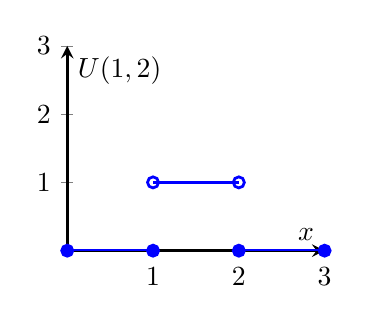
\begin{tikzpicture}
        \begin{axis}[axis x line={middle},
        axis y line={middle},
        ymax={3},
        xlabel={$x$},
        ylabel={$U(1,2)$},
        xmin={0},
        ymin={0},
        line width=1pt,
        width=0.4\textwidth
        ]
         \addplot+ [mark=o,] coordinates { (1,1) (2,1)};
         \addplot [blue,mark=*,] coordinates { (0,0) (1,0)};
         \addplot [blue,mark=*,] coordinates { (2,0) (3,0)};
        \end{axis}
    \end{tikzpicture}
    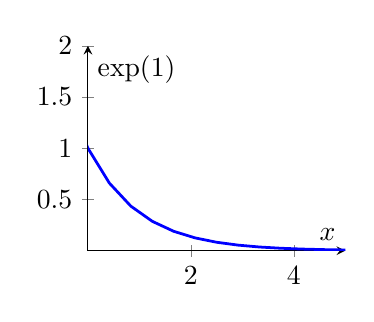
\begin{tikzpicture}
        \begin{axis}[axis x line={middle},
        axis y line={middle},
        xlabel={$x$},
        ylabel={$\exp(1)$},
        xmin={0},
        ymin={0},
        ymax={2},
        width=0.4\textwidth
        ]
         \addplot+ [no markers,line width=1pt,] {exp(-x)};
        \end{axis}
    \end{tikzpicture}
    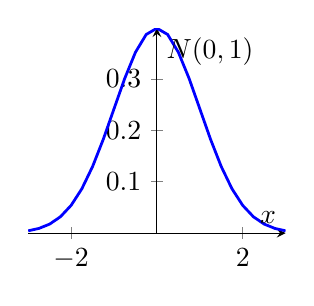
\begin{tikzpicture}
        \begin{axis}[axis x line={middle},
        axis y line={middle},
        ymax={},
        xlabel={$x$},
        ylabel={$N(0,1)$},
        xmin={},
        ymin={0},
        width=0.4\textwidth
        ]
            \addplot+ [no markers,domain=-3:3,line width=1pt,] {1/(sqrt(2*pi))*exp(-x^2/2)};
        \end{axis}
    \end{tikzpicture}
\end{figure}

\begin{proposition}[分布函数法]
    设 $(X,Y)\sim f(x,y)$,$Z=g(X,Y)$,则
    \begin{equation}
        F_Z(z)=P\{g(X,Y)\leq z\}=\iint_{g(x,y)\leq z}f(x,y)\diff x\diff y
    \end{equation}
\end{proposition}

\begin{proposition}[卷积公式法]
    设 $(X,Y)\sim f(x,y)$,$\overset{d}{=}$ 表示变量独立的条件下。
    \begin{enumerate}
        \item $Z=X+Y$ 的概率密度为
        \begin{equation}
            f_Z(z)=\int_{-\infty}^{+\infty}f(x,z-x)\diff y\overset{d}{=}\int_{-\infty}^{+\infty}f_X(x)f_Y(z-x)\diff x\overset{\triangle}{=}f_X(z)*f_Y(z)
        \end{equation}
        \item $Z=X-Y$ 的概率密度为
        \begin{equation}
            f_Z(z)=\int_{-\infty}^{+\infty}f(x,x-z)\diff y\overset{d}{=}\int_{-\infty}^{+\infty}f_X(x)f_Y(x-z)\diff x
        \end{equation}
        \item $Z=XY$ 的概率密度为
        \begin{equation}
            f_Z(z)=\int_{-\infty}^{+\infty}\frac{1}{|x|}f\left(x,\frac{z}{x}\right)\overset{d}{=}\int_{-\infty}^{+\infty}\frac{1}{|x|}f_X(x)f_Y\left(\frac{z}{x}\right)\diff x
        \end{equation}
        \item $Z=\frac{X}{Y}$ 的概率密度为
        \begin{equation}
            f_Z(z)=\int_{-\infty}^{+\infty}|y|f(yz,y)\diff y\overset{d}{=}\int_{-\infty}^{+\infty}|y|f_X(yz)f_Y(y)\diff y
        \end{equation}
        \item $Z=\max\{X,Y\}$ 的分布函数为
        \begin{equation}
            F_Z(z)=F(z,z)\overset{d}{=}F_X(z)\cdot F_Y(z)
        \end{equation}
        \item $Z=\min\{X,Y\}$ 的分布函数为
        \begin{equation}
            F_Z(z)=F_X(z)+F_Y(z)-F(z,z)\overset{d}{=}1-[1-F_X(z)][1-F_Y(z)]
        \end{equation}
    \end{enumerate}
\end{proposition}

\begin{theorem}[可加性]
    \begin{align}
        X&\sim B(n_1,p) & Y&\sim B(n_2,p) && X+Y\sim B(n_1+n_2,p) \\
        X&\sim \pi(\lambda_1) & Y&\sim \pi(\lambda_2) && X+Y\sim \pi(\lambda_1+\lambda_2)\\
        X&\sim N(\mu_1,\sigma_1^2) & Y&\sim N(\mu_2,\sigma_2^2) && X+Y\sim N(\mu_1\pm \mu_2,\sigma_1^2+\sigma_2^2)\\
        \chi_1^2&\sim\chi^2(n_1) & \chi_2^2&\sim\chi^2(n_2) && \chi_1^2+\chi_2^2\sim\chi^2(n_1+n_2) \marginnote{$\chi^2=\sum_{i=1}^n X_i^2$}
    \end{align}
\end{theorem}

\begin{definition}[期望]
    \begin{align}
        E(X)&=\int_{-\infty}^{+\infty}xf(x)\diff x\\
        E(Y)&=E(g(X))=\int_{-\infty}^{+\infty}g(x)f(x)\diff x\\
        E(Z)&=E(g(X,Y))=\int_{-\infty}^{+\infty}\int_{-\infty}^{+\infty}g(x,y)f(x,y)\diff x\diff y\\
        E(aX+bY)&=aEX+bEY\\
        E(XY)&=EXEY \tag{X,Y 独立}
    \end{align}
\end{definition}

\begin{definition}[方差]
    \begin{align}
        D(X)&=EX^2-(EX)^2\\
        D(aX+b)&=a^2DX\\
        D(X\pm Y)&=DX+DY\pm 2\textnormal{cov}(X,Y)\\
        D(X)&\leq E((X-c)^2)\quad\forall c\in\mathbb{R}
    \end{align}
\end{definition}

\begin{definition}[协方差]
    \begin{align}
        \textnormal{cov}(X,Y)&=E[(X-E(X))(Y-E(Y))]\\
        &=E(XY)-EXEY\\
        \textnormal{cov}(X+Y,Z)&=\textnormal{cov}(X,Z)+\textnormal{cov}(Y,Z)\\
        \rho_{XY}&=\frac{\textnormal{cov}(X,Y)}{\sqrt[]{DX}\sqrt[]{DY}}
    \end{align}
\end{definition}

\chapter{大数定律、中心极限定理}

\begin{definition}[依概率收敛]
    设 $\{Y_n\}$ 是一个随机变量序列(简称随机序列),$a$ 是常数,若对任意的 $\epsilon>0$,有
    \begin{equation}
        \lim_{n\rightarrow\infty}P(|Y_n-a|<\epsilon)=1
    \end{equation}
    则称随机序列 $\{Y_n\}$ 依概率收敛于 $a$,记作 $Y_n\xrightarrow{P} a$。
\end{definition}

\begin{theorem}[Chebyshev 不等式]
    设随机变量 $X$ 具有数学期望 $E(X)=\mu$,方差 $D(X)=\sigma^2$,则对于任意整数 $\epsilon$,恒有不等式
    \begin{equation}
        P(|X-\mu|<\epsilon)>1-\frac{\sigma^2}{\epsilon^2}
    \end{equation}
\end{theorem}

\begin{theorem}[Chebyshev 大数定律]
    设 $\{X_n\}$ 为两两互不相关的随机序列,若它们的方差存在,且有共同的上界,即存在常数 $c$,$D(X_i)\leq c$ 对 $\forall i\geq 1$ 成立\marginpar{可放松条件为 Markov 条件:\begin{equation}\frac{1}{n^2}D\left(\sum_{i=1}^n X_i\right)\rightarrow 0\end{equation}},则 $\{X_n\}$ 服从大数定律,即对任意的 $\epsilon>0$,有
    \begin{equation}
        \frac{1}{n}\sum_{i=1}^nX_i\xrightarrow[]{P}\frac{1}{n}\sum_{i=1}^n E(X_i)
    \end{equation}
\end{theorem}

\begin{theorem}[Bernoulli 大数定律]
    设 $\xi_n$ 是 $n$ 重 Bernoulli 试验中事件 $A$ 发生的次数,$p$ 为每次实验中 $A$ 发生的概率,则对任意的 $\epsilon>0$,有
    \begin{equation}
        \lim_{n\rightarrow\infty}P\left(\left|\frac{\xi_n}{n}-p\right|<\epsilon\right)=1
    \end{equation}
\end{theorem}

\begin{theorem}[Khintchine 大数定律]
    假设 $\{X_n\}$ 是独立同分布的随机变量序列,如果数学期望存在,则对任意的 $\epsilon>0$,有
    \begin{equation}
        \lim_{n\rightarrow\infty}P\left(\left|\frac{1}{n}\sum_{i=1}^n X_i-\frac{1}{n}\sum_{i=1}^n E(X_i)\right|<\epsilon\right) = 1
    \end{equation}
\end{theorem}

\begin{theorem}[Lindeberg--L\'evy 中心极限定理,独立同分布中心极限定理]
    设 $\{X_n\}$ 为独立的随机序列,且 $E(X_i)=\mu, D(X_i)=\sigma^2>0$,记
    \begin{equation}
        Y_n^*=\frac{\sum_{k=1}^n X_k-n\mu}{\sigma\sqrt{n}}
    \end{equation}
    则对任意实数 $y$,有
    \begin{equation}\label{eq:central}
        \lim_{n\rightarrow\infty}P(Y_n^*\leq y)=\frac{1}{\sqrt{2\pi}}\int_{-\infty}^y\e^{-\frac{x^2}{2}}\diff x=\Phi(y)
    \end{equation}
\end{theorem}

\begin{theorem}[De Moivre--Laplace 中心极限定理]
    \marginpar{该定理表明,正态分布是二项分布的极限分布。}
    设随机变量 $\xi_n\sim B(n,p)$,$(0<p<1)$,记
    \begin{equation}
        Y_n^*=\frac{\xi_n-np}{\sqrt[]{np(1-p)}}
    \end{equation}
    则对任意实数 $y$,有 \eqref{eq:central} 成立。
\end{theorem}

\chapter{统计量及其分布}

\begin{definition}[统计量]
    设 $X_1,X_2,\cdots,X_n$ 为取自总体 $X$ 的一个样本,若样本函数 $T=g(X_1,X_2,\cdots,X_n)$ 中不含有任何未知参数,则称 $T$ 为统计量。
    \begin{description}
        \item[样本原点矩]
        \begin{equation}\label{eq:orimoment}
            A_r=\frac{1}{n}\sum_{i=1}^n X_i^r
        \end{equation}
        \item[样本均值]
        当 \eqref{eq:orimoment} 中 $r=1$ 时,称为样本均值
        \begin{equation}
            \bar{X}=A_1=\frac{1}{n}\sum_{i=1}^n X_i
        \end{equation}
        \item[样本中心矩]
        \begin{equation}\label{eq:cenmoment}
            a_r=\frac{1}{n}\sum_{i=1}^n (X_i-\bar{X})^r
        \end{equation}
        当 \eqref{eq:cenmoment} 中 $r=2$ 时,为二阶中心矩。\marginpar{二阶中心矩有偏,$ES_n^2=\frac{n-1}{n}\sigma^2$;又言,因为减去了均值,所以自由度变为了 $n-1$,$\bar{X}$ 所反映的量是未知的。}
        \item[样本方差]
        \begin{equation}
            S^2=\frac{1}{n-1}\sum_{i=1}^n (X_i-\bar{X})^2 
        \end{equation}
        为样本方差,其算数根 $S=\sqrt{S^2}$ 称为样本标准差。
    \end{description}
\end{definition}

\begin{definition}[顺序统计量]
    设 $X_1,X_2,\cdots,X_n$ 为来自总体 $X$ 的一个样本,一次抽取观察值为 $(x_1,x_2,\cdots,x_n)$,此时将观察值的各个分量按照其值的大小从小到大重新排列,
    \begin{equation}
        x_{(1)}\leq x_{(2)}\leq \cdots \leq x_{(n)}
    \end{equation}
    定义 $X_{(k)}$ 的取值为 $x_{(k)}$,称
    \begin{equation}
        (X_{(1)}, X_{(2)}, \cdots , X_{(n)})
    \end{equation}
    为样本的顺序统计量。显然有
    \begin{equation}
        \min_{1\leq k\leq n}\{X_k\}=X_{(1)}\leq X_{(2)}\leq \cdots \leq X_{(n)}=\max_{1\leq k\leq n}\{X_k\}
    \end{equation}
    称
    \begin{equation}
        \tilde{x}=\begin{cases}
            x_{(\frac{n+1}{2})},&n\text{为奇数}\\
            [x_{(\frac{n}{2})}+x_{(\frac{n}{2}+1)}]/2,&n\text{为偶数}
        \end{cases}
    \end{equation}
    为样本观察值的中位数。
\end{definition}

\begin{definition}[分位点]
    设随机变量 $X$ 的密度为 $f(x)$,若对任意给定的 $\alpha(0<\alpha<1)$,存在实数 $x_\alpha\in\mathbb{R}$,满足
    \begin{equation}
        P(X>x_\alpha)=\alpha
    \end{equation}
    则称 $x_\alpha$ 为该分布的 $\alpha$ 上侧分位点。若对任意给定的 $\gamma$,存在实数 $y_\gamma\in\mathbb{R}$,满足
    \begin{equation}
        P(X\leq y_\gamma)=1-\gamma
    \end{equation}
    则称 $y_\gamma$ 为该分布的下侧分位点。使用分位数时只采用上侧分位点,或称单侧分位点。

    设随机变量 $X$ 的密度 $f(x)$ 为偶函数,若对任意给定的 $\alpha(0<\alpha<1)$,存在实数 $x_{\alpha/2}\in\mathbb{R}$,满足
    \begin{equation}
        P(|X|>x_{\alpha/2})=\alpha
    \end{equation}
    则称 $x_{\alpha/2}$ 为该分布的 $\alpha$ 双侧分位点。
\end{definition}

\begin{definition}[正态分布]
    \begin{equation}
        f(x)=\frac{1}{\sqrt{2\pi}\sigma}\e^{-\frac{1}{2}\left(\frac{x-\mu}{\sigma}\right)^2}
    \end{equation}
    \begin{equation}
        f(x,y)=\frac{1}{2\pi\sigma_1\sigma_2\sqrt{1-\rho^2}}\e^{-\frac{1}{2(1-p^2)}\left[\left(\frac{x-\mu_1}{\sigma_1}\right)^2-2\rho\frac{x-\mu_1}{\sigma_1}\frac{y-\mu_2}{\sigma_2}+\left(\frac{y-\mu_2}{\sigma_2}\right)^2\right]}
    \end{equation}
\end{definition}

\begin{definition}[$\chi^2$ 分布]
    设 $(X_1,X_2,\cdots,X_n)$ 为来自总体 $X\sim N(0,1)$ 的一个样本,则称
    \begin{equation}
        \chi^2=\sum_{i=1}^n X_i^2
    \end{equation}
    为 $\chi^2$ 统计量,且服从自由度为 $n$ 的 $\chi^2$ 分布,记作 $\chi^2\sim\chi^2(n)$。自由度 $n$ 是指独立随机变量的个数。

    \begin{description}
        \item[可加性] 若 $\chi^2_1\sim\chi^2(n_1), \chi^2_2\sim\chi^2(n_2)$,且 $\chi_1^2$ 与 $\chi_2^2$ 相互独立,则
        \begin{equation}
            \chi_1^2+\chi_2^2\sim\chi^2(n_1+n_2)
        \end{equation}
        \item[期望与方差] 若 $\chi^2\sim\chi^2(n)$,则 
        \begin{align}
            E(\chi^2)&=n\\
            D(\chi^2)&=2n
        \end{align}
    \end{description}
\end{definition}

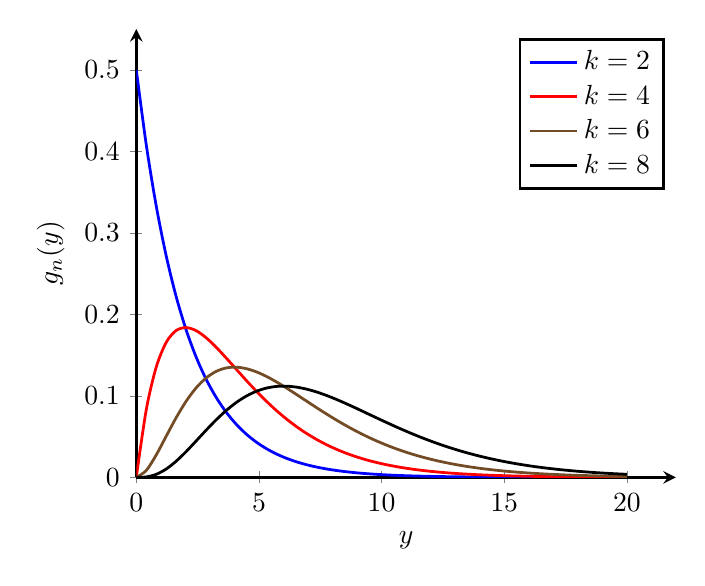
\begin{tikzpicture}[
    declare function={gamma(\z)=
    (2.506628274631*sqrt(1/\z) + 0.20888568*(1/\z)^(1.5) + 0.00870357*(1/\z)^(2.5) - (174.2106599*(1/\z)^(3.5))/25920 - (715.6423511*(1/\z)^(4.5))/1244160)*exp((-ln(1/\z)-1)*\z);},
    declare function={gammapdf(\x,\k,\theta) = \x^(\k-1)*exp(-\x/\theta) / (\theta^\k*gamma(\k));}
]

\begin{axis}[
    axis lines=left,
    enlargelimits=upper,
    samples=50,
    legend entries={$k=2$,$k=4$,$k=6$,$k=8$},
    line width=1,
    no markers,
    smooth, domain=0:20,
    xlabel={$y$},
    ylabel={$g_n(y)$}
]
\addplot+ {gammapdf(x,1,2)};
\addplot+ {gammapdf(x,2,2)};
\addplot+ {gammapdf(x,3,2)};
\addplot+ {gammapdf(x,4,2)};
\end{axis}
\end{tikzpicture}

\begin{definition}[$t$ 分布]
    设 $X=N(0,1), Y\sim \chi^2(n)$ 且 $X$ 与 $Y$ 相互独立,则称
    \begin{equation}
        T=\frac{X}{\sqrt{Y/n}}
    \end{equation}
    为 $T$ 统计量,且服从自由度为 $n$ 的 $t$ 分布,记作 $T\sim t(n)$。
\end{definition}

\begin{definition}[$F$ 分布]
    设 $U\sim\chi^2(m), V\sim\chi^2(n)$,且 $U$ 与 $V$ 相互独立,则称
    \begin{equation}
        F=\frac{U/m}{V/n}
    \end{equation}
    为 $F$ 统计量,且服从第一自由度为 $m$ 和第二自由度为 $n$ 的 $F$ 分布,记作 $F\sim F(m,n)$。

    \begin{enumerate}
        \item 若 $F\sim F(m,n)$,则 $\frac{1}{F}\sim F(n,m)$;
        \item \begin{equation}
            F_{1-\alpha}(m,n)=\frac{1}{F_\alpha(n,m)}
        \end{equation}
    \end{enumerate}
\end{definition}

\begin{theorem}[正态总体下的常用结论]
    设 $(X_1,X_2,\cdots,X_n)$ 为来自总体 $N(\mu,\sigma^2)$ 的一个样本,则样本均值 $\bar{X}$ 与样本方差 $S^2$ 相互独立,
    \begin{align}
        \bar{X}&\sim N(\mu,\frac{\sigma^2}{n})\\
        \frac{\bar{X}-\mu}{\sigma/\sqrt{n}}&\sim N(0,1)\\
        \frac{1}{\sigma^2}\sum_{i=1}^n(X_i-\mu)^2&\sim\chi^2(n)\\
        \frac{S_n^2}{\sigma^2}=\frac{(n-1)S^2}{\sigma^2}=\sum_{i=1}^n\left(\frac{X_i-\bar{X}}{\sigma}\right)^2&\sim\chi^2(n-1)\\
        \frac{\bar{X}-\mu}{S/\sqrt{n}}&\sim t(n-1)\\
        \frac{(\bar{X}-\mu)^2}{S^2/n}&\sim F(1,n-1)
    \end{align}
\end{theorem}

\chapter{参数估计与假设检验}

\begin{definition}[矩估计法]
    通过原点矩 $A_k=\frac{1}{n}\sum_{i=1}^n X_i^k$ 估计总体原点矩 $E(X^k)$。
    \begin{equation}
        \begin{cases}
            \mu_1=E(X)\\
            \mu_2=E(X^2)
        \end{cases}
    \end{equation}
\end{definition}

\begin{definition}[最大似然估计]
    概率最大的随机事件在一次试验中最可能发生。
    \begin{align}
        L(x_1,x_2,\cdots,x_n;\theta)&=\prod_{i=1}^n p(x_i;\theta) & L(x_1,x_2,\cdots,x_n;\theta) &= \prod_{i=1}^n f(x_i;\theta)\\
        \frac{\partial L(\theta)}{\partial \theta_i}&=0 & \frac{\partial \ln L(\theta)}{\partial \theta_i}&=0\\
        \hat{\theta}_i&=\theta_i^*
    \end{align}
    若似然方程组有唯一解并且该解不是在未知参数的取值范围的边界上取得的,那么该解就是最大点。
\end{definition}

\begin{definition}[估计量的评价标准]
    不同的估计量 $\hat{\theta}$ 的评价标准。
    \begin{description}
        \item[无偏性] 设参数 $\theta$ 的估计量为 $\hat{\theta}=\hat{\theta}(X_1,X_2,\cdots,X_n)$,若有
        \begin{equation}
            E(\hat{\theta})=\theta
        \end{equation}
        则称 $\hat{\theta}$ 是 $\theta$ 的无偏估计量。反之,称 $\epsilon=E(\hat{\theta})-\theta$ 为估计量 $\theta$ 的偏差。
        \item[有效性] 设 $\hat{\theta}_1=\hat{\theta}_1(X_1,X_2,\cdots,X_n)$ 和 $\hat{\theta}_2$ 均为 $\theta$ 的无偏估计量,对任意 $n$ 有
        \begin{equation}
            D(\hat{\theta}_1)<D(\hat{\theta}_2)
        \end{equation}
        则称 $\hat{\theta}_1$ 比 $\hat{\theta}_2$ 有效。如果方差是所有的里面最小的,则称为有效估计量。
        \item[一致性] 设 $\hat{\theta}_n=\hat{\theta}_n(X_1,X_2,\cdots,X_n)$ 为未知参数 $\theta$ 的估计量,如果序列 $\{\hat{\theta}_n\}$ 依概率收敛于 $\theta$,即 $\forall\epsilon>0$,有
        \begin{equation}
            \lim_{n\rightarrow\infty} P(|\hat{\theta_n}-\theta|<\epsilon)=1
        \end{equation}
        则称 $\hat{\theta_n}$ 是 $\theta$ 的一致估计量(相合估计量)。
    \end{description}
\end{definition}

\begin{theorem}[一致估计量判别法]
    设 $\hat{\theta}_n=\hat{\theta}_n(X_1,X_2,\cdots,X_n)$ 为未知参数 $\theta$ 的无偏估计量,若
    \begin{equation}
        \lim_{n\rightarrow\infty}D(\hat{\theta}_n)=0
    \end{equation}
    则 $\hat{\theta}_n$ 是 $\theta$ 的一致估计量。
\end{theorem}

\begin{definition}[置信区间]
    设总体 $X$ 的分布 $F(x;\theta)$ 含有一个未知参数 $\theta$,并且 $(X_1,X_2,\cdots,X_n)$ 为来自总体 $X$ 的一个样本。若 $\forall\alpha(0<\alpha<1)$,存在 $\hat{\theta}_1=\hat{\theta}_1(X_1,X_2,\cdots,X_n)$ 和 $\hat{\theta}_2=\hat{\theta}_2(X_1,X_2,\cdots,X_n)$,使得 $P(\hat{\theta}_1<\theta<\hat{\theta}_2)=1-\alpha$ 成立。则称区间 $(\hat{\theta_1},\hat{\theta_2})$ 是 $\theta$ 的置信度为 $1-\alpha$ 的置信区间,$\theta_1$ 和 $\theta_2$ 分别称为置信下限与置信上限。$\alpha$ 被称为显著性水平。
\end{definition}

\begin{proposition}[估计正态分布中 $\mu$ 的置信区间]
    已知置信度为 $1-\alpha$,$(X_1,X_2,\cdots,X_n)$ 为来自正态总体 $N(\mu,\sigma^2)$ 的一个样本,
    \marginpar{如果讨论单侧置信限,则将 $\frac{\alpha}{2}\rightarrow\alpha$。}
    \begin{enumerate}
        \item 方差 $\sigma^2$ 已知,
        \begin{equation}
            \left(\bar{X}-u_{\frac{\alpha}{2}}\frac{\sigma}{\sqrt{n}},\bar{X}+u_{\frac{\alpha}{2}}\frac{\sigma}{\sqrt{n}}\right)
        \end{equation}
        \item 方差 $\sigma^2$ 未知,
        \begin{equation}
            \left(\bar{X}-t_{\frac{\alpha}{2}}(n-1)\frac{S}{\sqrt{n}},\bar{X}+t_{\frac{\alpha}{2}}(n-1)\frac{S}{\sqrt{n}}\right)
        \end{equation}
    \end{enumerate}
\end{proposition}

\begin{definition}[两类错误]
    由于假设检验采用了 “小概率事件在一次试验中几乎不可能发生” 这一实际推断原理,这就决定了假设检验可能会犯错。
    \begin{description}
        \item[“弃真” $\alpha$] 实际上 $H_0$ 为真,但是却错误地拒绝了 $H_0$。
        \item[“取伪” $\beta$] 实际上 $H_0$ 为假,但是却错误地接受了 $H_0$。
    \end{description}
    
    \begin{tabular}{ccc}
         & 接受 $H_0$ & 接受 $H_1$ \\
        $H_0$ 为真 & 正确($1-\alpha$) & 第 I 类错误($\alpha$) \\
        $H_0$ 为假 & 第 II 类错误($\beta$) & 正确($1-\beta$)
    \end{tabular}
\end{definition}

\begin{proposition}[正态分布下的六大检验]
    设样本 $(X_1,X_2,\cdots,X_n)$ 来自正态总体 $N(\mu,\sigma^2)$。
    
    \noindent\begin{tabular}{ccccll}
        $\sigma^2$ & $\mu$ & $H_0$ & $H_1$ & 分布 &拒绝域 \\
        \hline
        已知 & 未知 & $\mu=\mu_0$ & $\mu\neq\mu_0$ & \multirow{3}{*}{$U=\frac{\bar{X}-\mu_0}{\frac{\sigma}{\sqrt{n}}}\sim N(0,1)$} & $|U|\geq u_{\frac{\alpha}{2}}$ \\
        已知 & 未知 & $\mu\leq\mu_0$ & $\mu>\mu_0$ & & $U\geq u_\alpha$ \\
        已知 & 未知 & $\mu\geq\mu_0$ & $\mu<\mu_0$ & & $U\leq -u_\alpha$ \\
        % $\left(-\infty,\mu_0-\frac{\sigma}{\sqrt{n}}u_{\frac{\alpha}{2}}\right]\cup\left[\mu_0+\frac{\sigma}{\sqrt{n}}u_{\frac{\alpha}{2}},+\infty\right)$\\
        \hline
        未知 & 未知 & $\mu=\mu_0$ & $\mu\neq\mu_0$ & \multirow{3}{*}{$T=\frac{\bar{X}-\mu_0}{\frac{S}{\sqrt{n}}}\sim t(n-1)$} & $|t|\geq t_{\frac{\alpha}{2}}(n-1)$ \\
        未知 & 未知 & $\mu\leq\mu_0$ & $\mu>\mu_0$ & & $t\geq t_\alpha(n-1)$\\
        未知 & 未知 & $\mu\geq\mu_0$ & $\mu<\mu_0$ & & $t\leq -t_\alpha(n-1)$
    \end{tabular}
\end{proposition}

\nocite{*}
\bibliography{ref}

\clearpage
\begin{multicols}{2}
    \small
    \listoftheorems
\end{multicols}

\end{document}